\chapter{Obesity associated genetic signatures and cancer}
\label{cha:obesity_genetic_signatures_and_cancer}

The obesity associated genetic signatures are central to this project in order to clarify the relationship between \gls{bmi} and cancer.
Firstly in this chapter, the previously identified obesity associated signatures from the studies conducted by \citet{Creighton2012} and \citet{Fuentes-Mattei2014} were examined in turn to judge the agreement of these signatures with the sample \gls{bmi}, as presented in thier results.
Secondly, novel obesity associated genetic signatures were identified in the \citet{Creighton2012} data set and was compared with the signatures.
Lastly, the presence of common genes or pathways that were associated with obesity in multiple types of cancer was explored using the \gls{icgc} cancer data sets.

\section{Obesity associated genetic signature from \citet{Creighton2012} study}
\label{sec:creighton_obesity_metagene}

Obesity metagene was created using the obesity associated genetic signatures from \citet{Creighton2012} study.
Since there was no description about the normalisation method used by Creighton's group, the \gls{rma} method was used to  normalise the Creighton data set.
The obesity metagene was plotted in a heatmap with the sample gene expression (\cref{fig:crmetaheat1}) to check whether the metagene scores were in accordance with the overall gene expression of the samples.

\begin{figure}[htb]
	\centering
	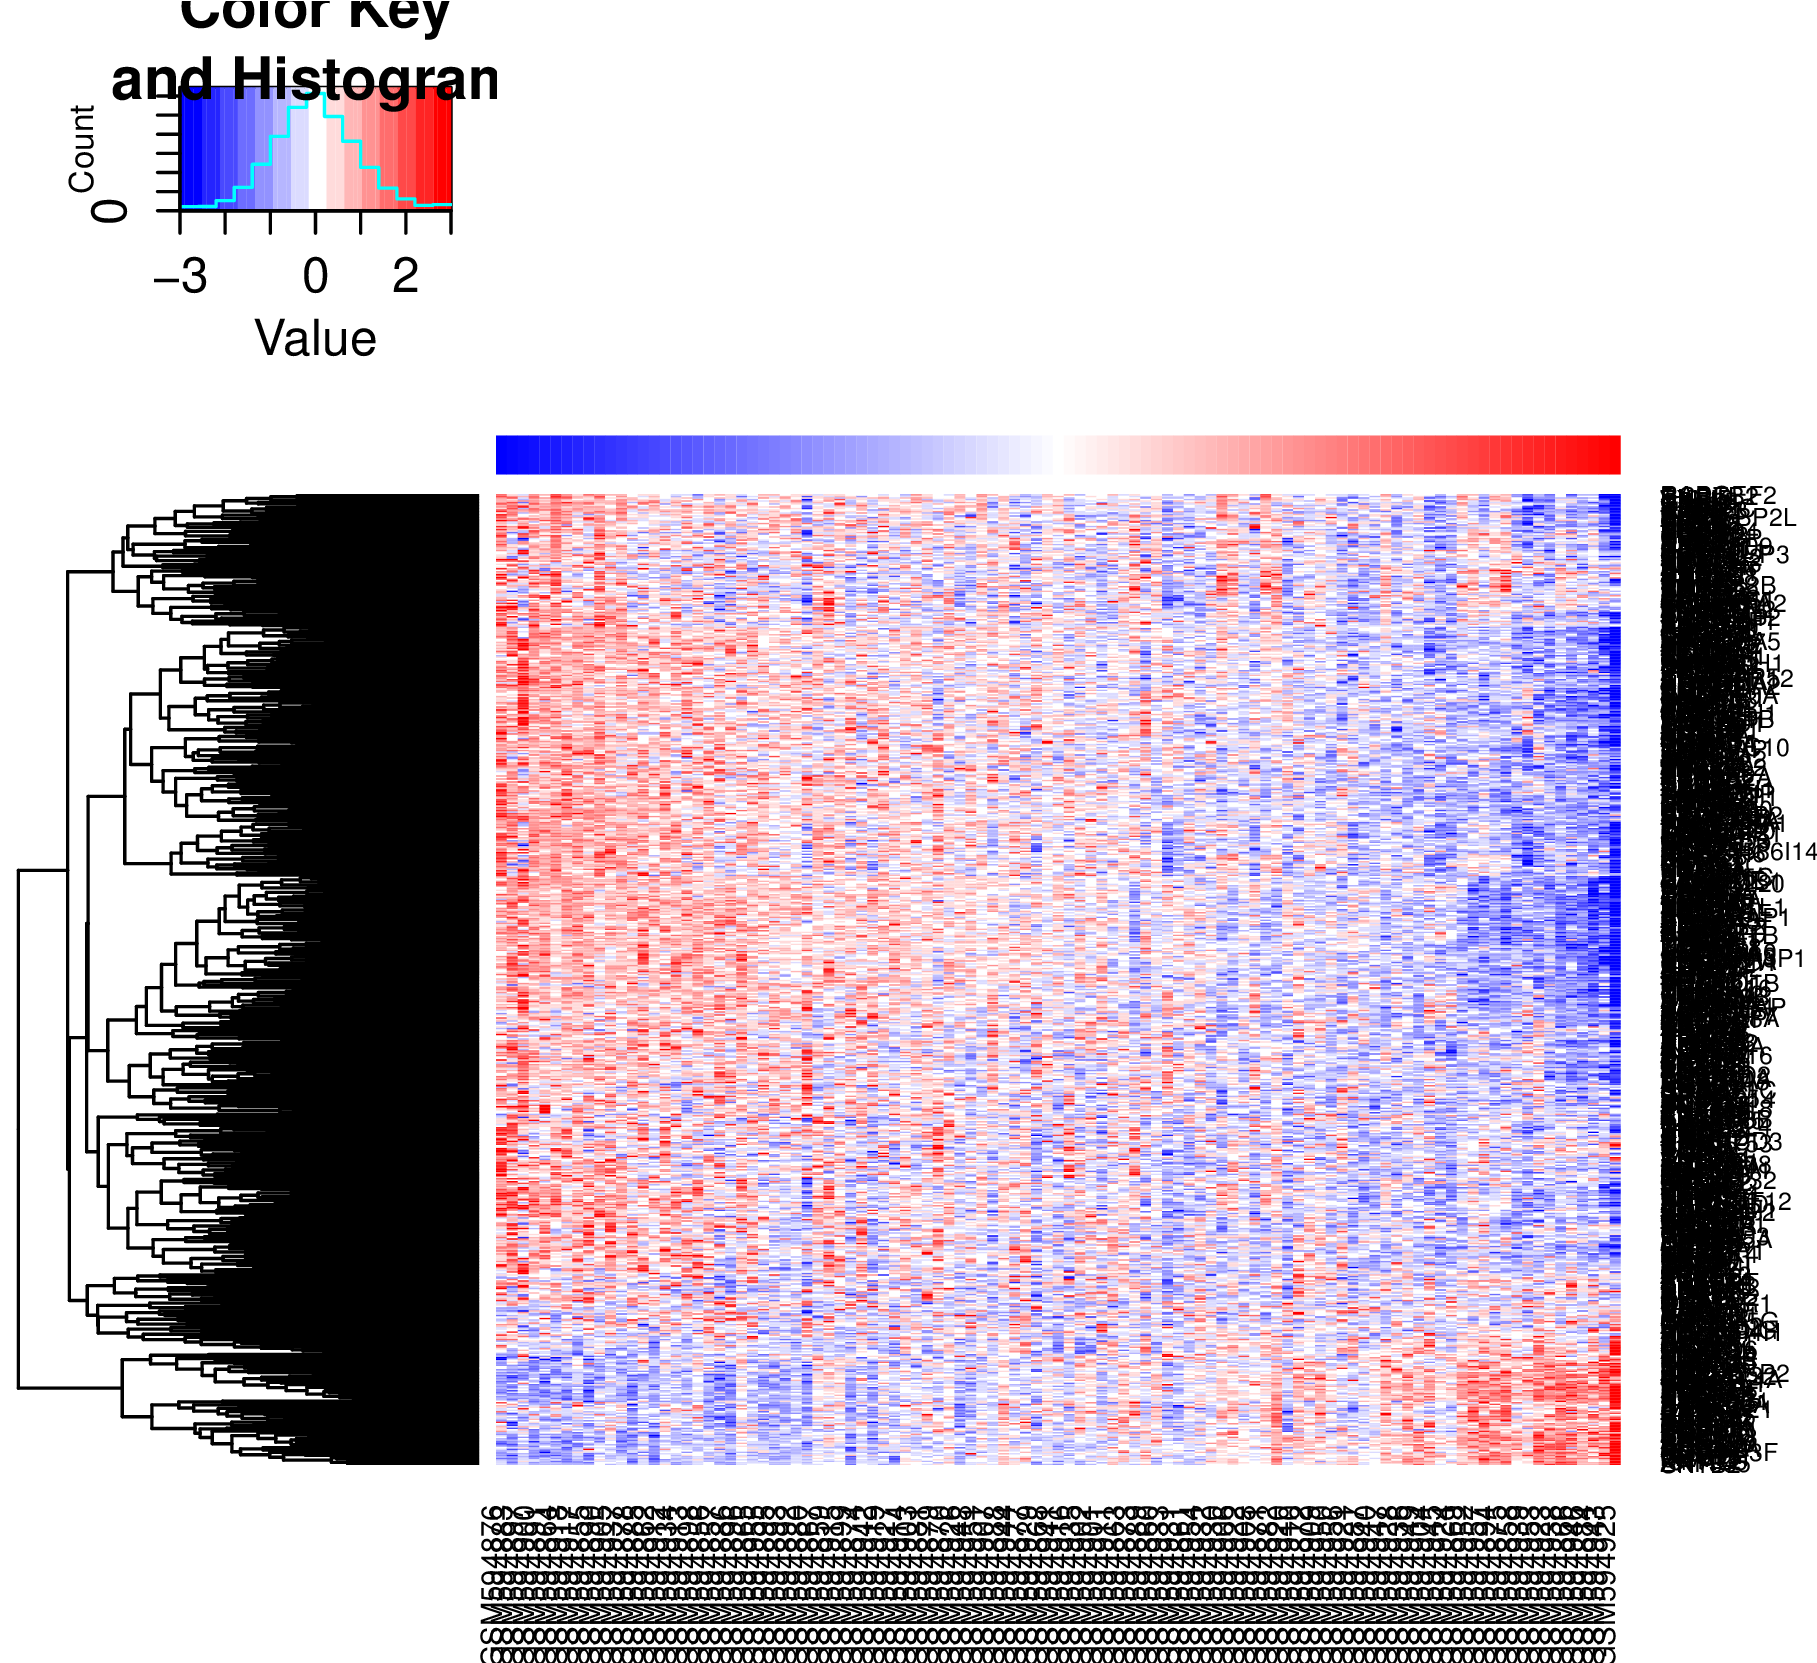
\includegraphics[width=0.8\linewidth]{results1/crmeta_original}
	\caption[Heatmap of Creighton's metagene in Creighton's data]{Heatmap showing Creighton's obesity associated metagene with the gene expressions of obesity associated genes in Creighton's data. Level of expression is represented in the top right histogram, where low and high gene expression were colour-coded with blue and red, respectively. Each row of the heatmap represents a gene from the obesity associated genetic signature, and each column of the heatmap represents a sample from Creighton's data. The obesity associated metagene scores of the samples are shown in a separate row at top of the heatmap, and the tree diagram of the heirarchical clustering of the genes is shown to the left of the heatmap. For clarity, the metagene scores were flipped in order to match the results from \citet{Creighton2012} paper.}
	\label{fig:crmetaheat1}
\end{figure}

As shown in \cref{fig:crmetaheat1}, high obesity associated metagene score of the sample reflected low expression in majority of the genes in the signature, and in contrast, low obesity associated metagene score of the sample reflected high expression in majority of the genes in the signature.
This was consistent with the reported property of the obesity associated signature by \citet{Creighton2012}.
To provide further evidence that the obesity associated metagenes were in fact associated with the \gls{bmi} status and \gls{bmi} value of the samples, a box plot and a scatter plot were created, respectively (\cref{fig:crmetaboxplot1}).

\begin{figure}[htp!]
	\centering
	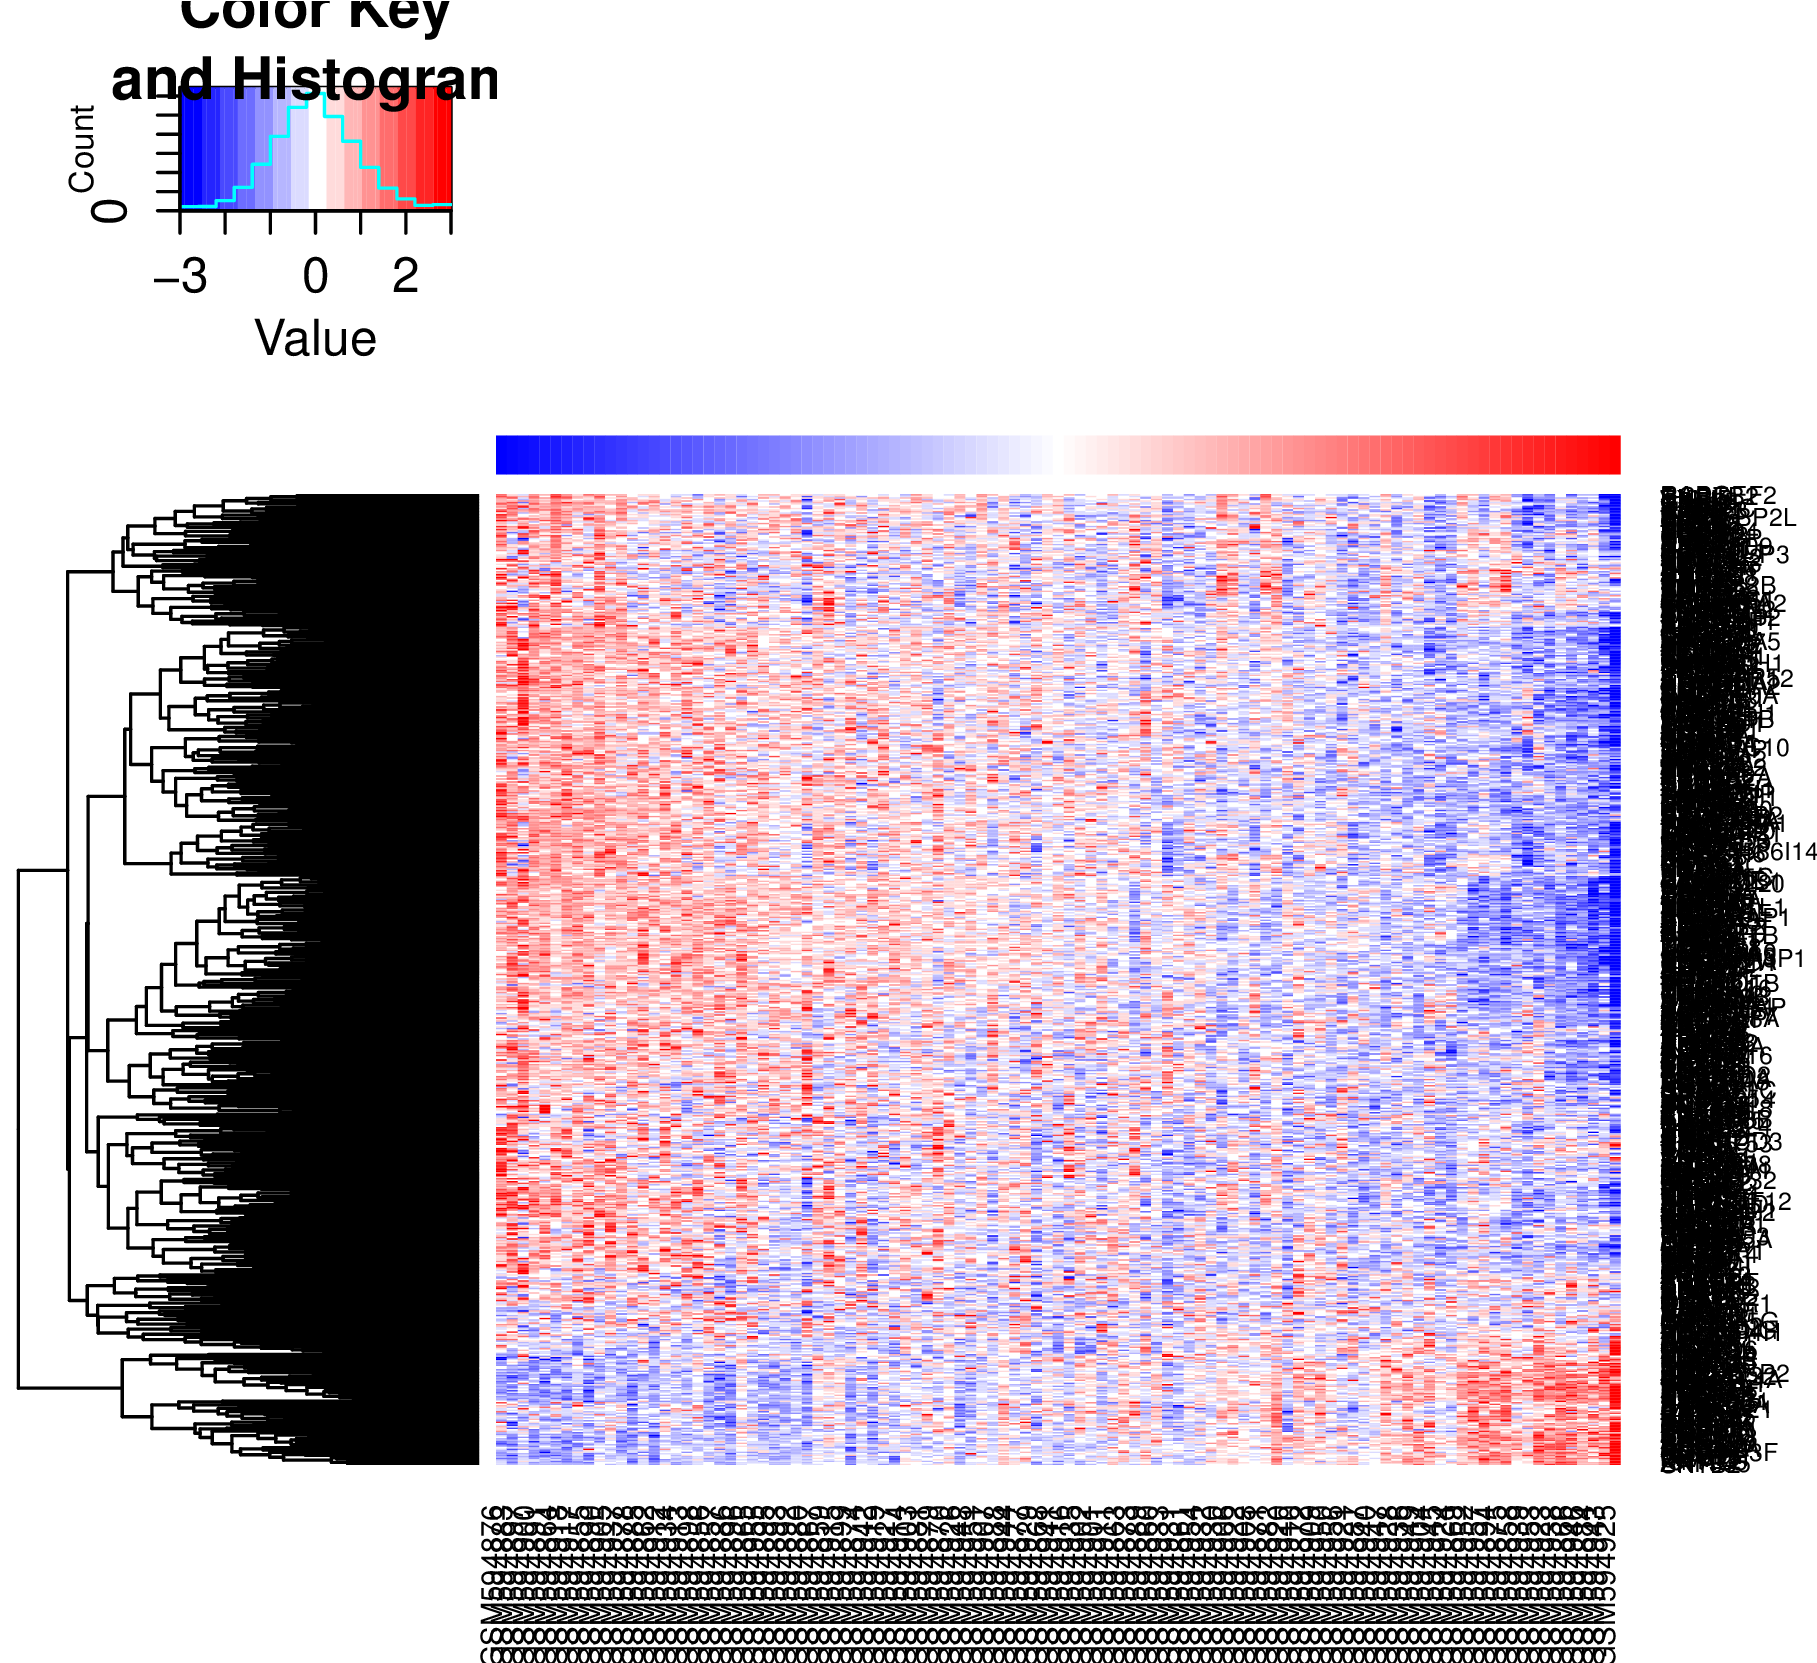
\includegraphics[width=0.45\linewidth]{results1/crmeta_original}
	\hfill
	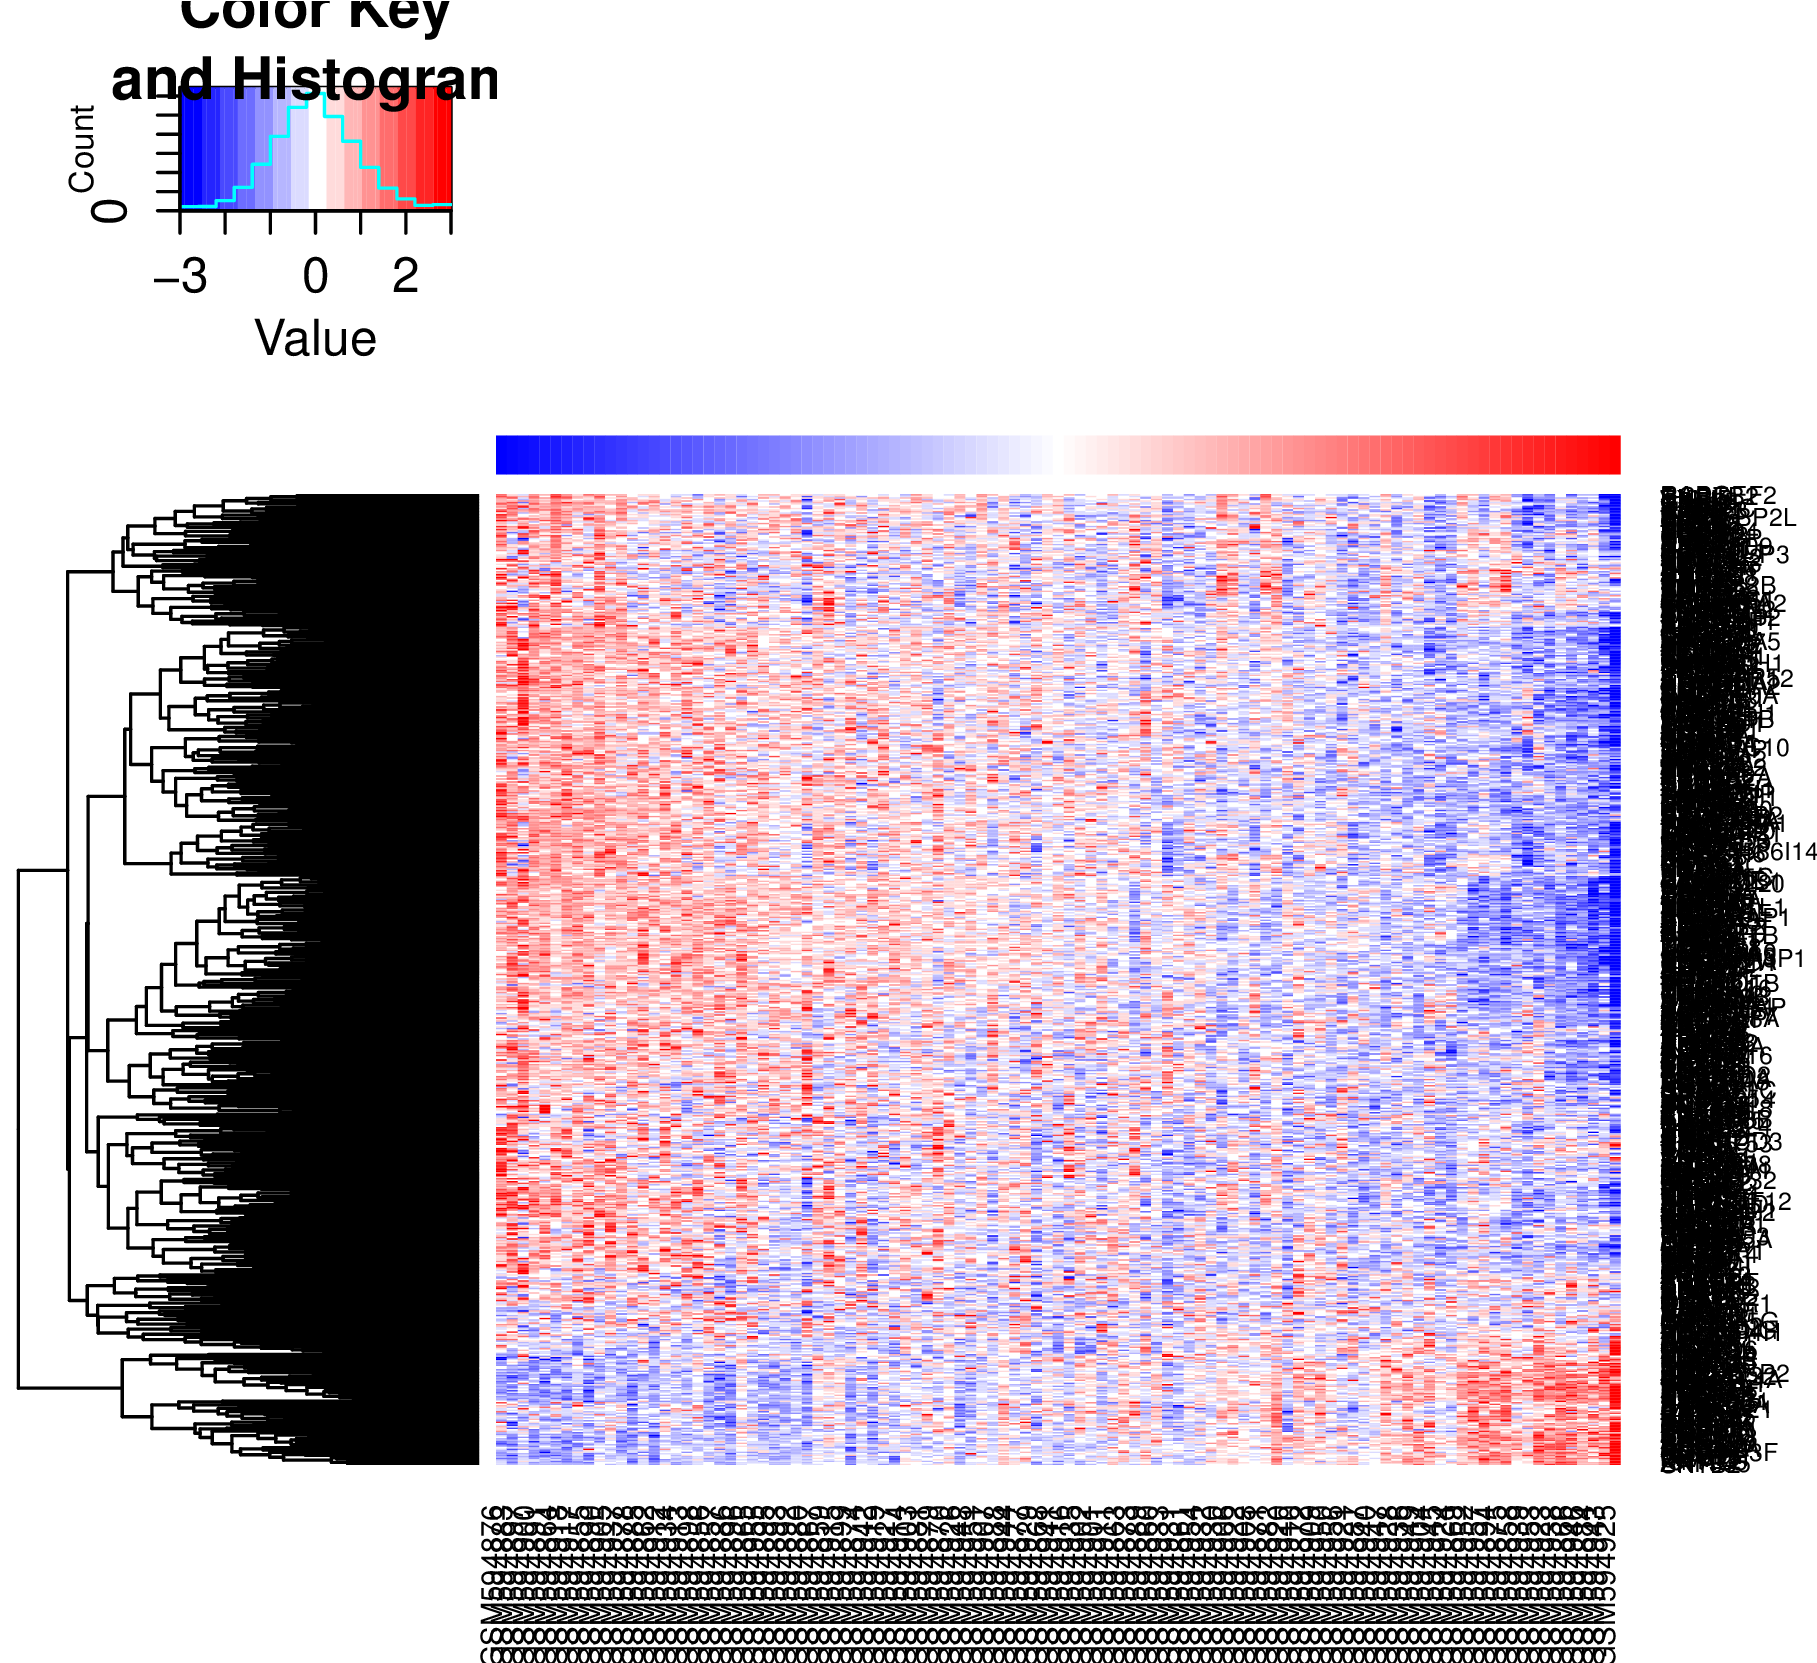
\includegraphics[width=0.45\linewidth]{results1/crmeta_original}
	\caption[Creighton metagene and sample \gls{bmi}/\gls{bmi} status]{(insert figure of box plot and scatter plot)}
	\label{fig:crmetaboxplot1}
\end{figure}

\cref{fig:crmetaboxplot1} clearly showed that the obesity associated metagene from \citet{Creighton2012} study significantly associated with the sample \gls{bmi} status, as well as the \gls{bmi} value of the samples (include p-value and r-squared).
It should be noted here that the obesity associated metagene significantly associated with the samples that were obese, but not the samples that were overweight.
This was due to the fact that the obesity associated genetic signatures were originally identified from the comparison of the samples that were obese with the samples that were not obese, and therefore the metagene scores were significant with obese group, but not the overweight group.
\\

\noindent
Now that the association of the obesity metagene from \citet{Creighton2012} study was established in Creighton's data set, the obesity associated signature was transferred to the \gls{icgc} cancer data.
The direction of the obesity associated metagene was checked in the Creighton's data, so that high metagene scores reflected high sample \gls{bmi} and low metagene scores reflected low sample \gls{bmi} (\cref{fig:crmetaboxplot1}).
The transformation matrix was created in Creighton's data, as described in \cref{sub:svd}.

All of the \gls{icgc} data were normalised as described in \cref{ssub:rna_seq_data}.
Before the transformation matrix was applied to the log$_{10}$-normalised cancer data, the suitability of standardised data or untouched (non-standardised) data was determined (appendix).
From these results, the standardised data was the most suitable to use for matrix transformation.
The transformation matrix was applied to each cancer data set in turn to obtain the obesity metagenes for each of the data set.
Each obesity metagenes were plotted on a heatmap with the corresponding data set in which the metagene was taken from \cref{fig:crmetaicgc1}.
These heatmaps confirmed that the obesity associated metagene derived from Creighton's data was able to capture the overall gene expression pattern, where the metagene scores reflected the expression levels of majority of the genes in the signature.

\begin{figure}[htp!]
	\centering
	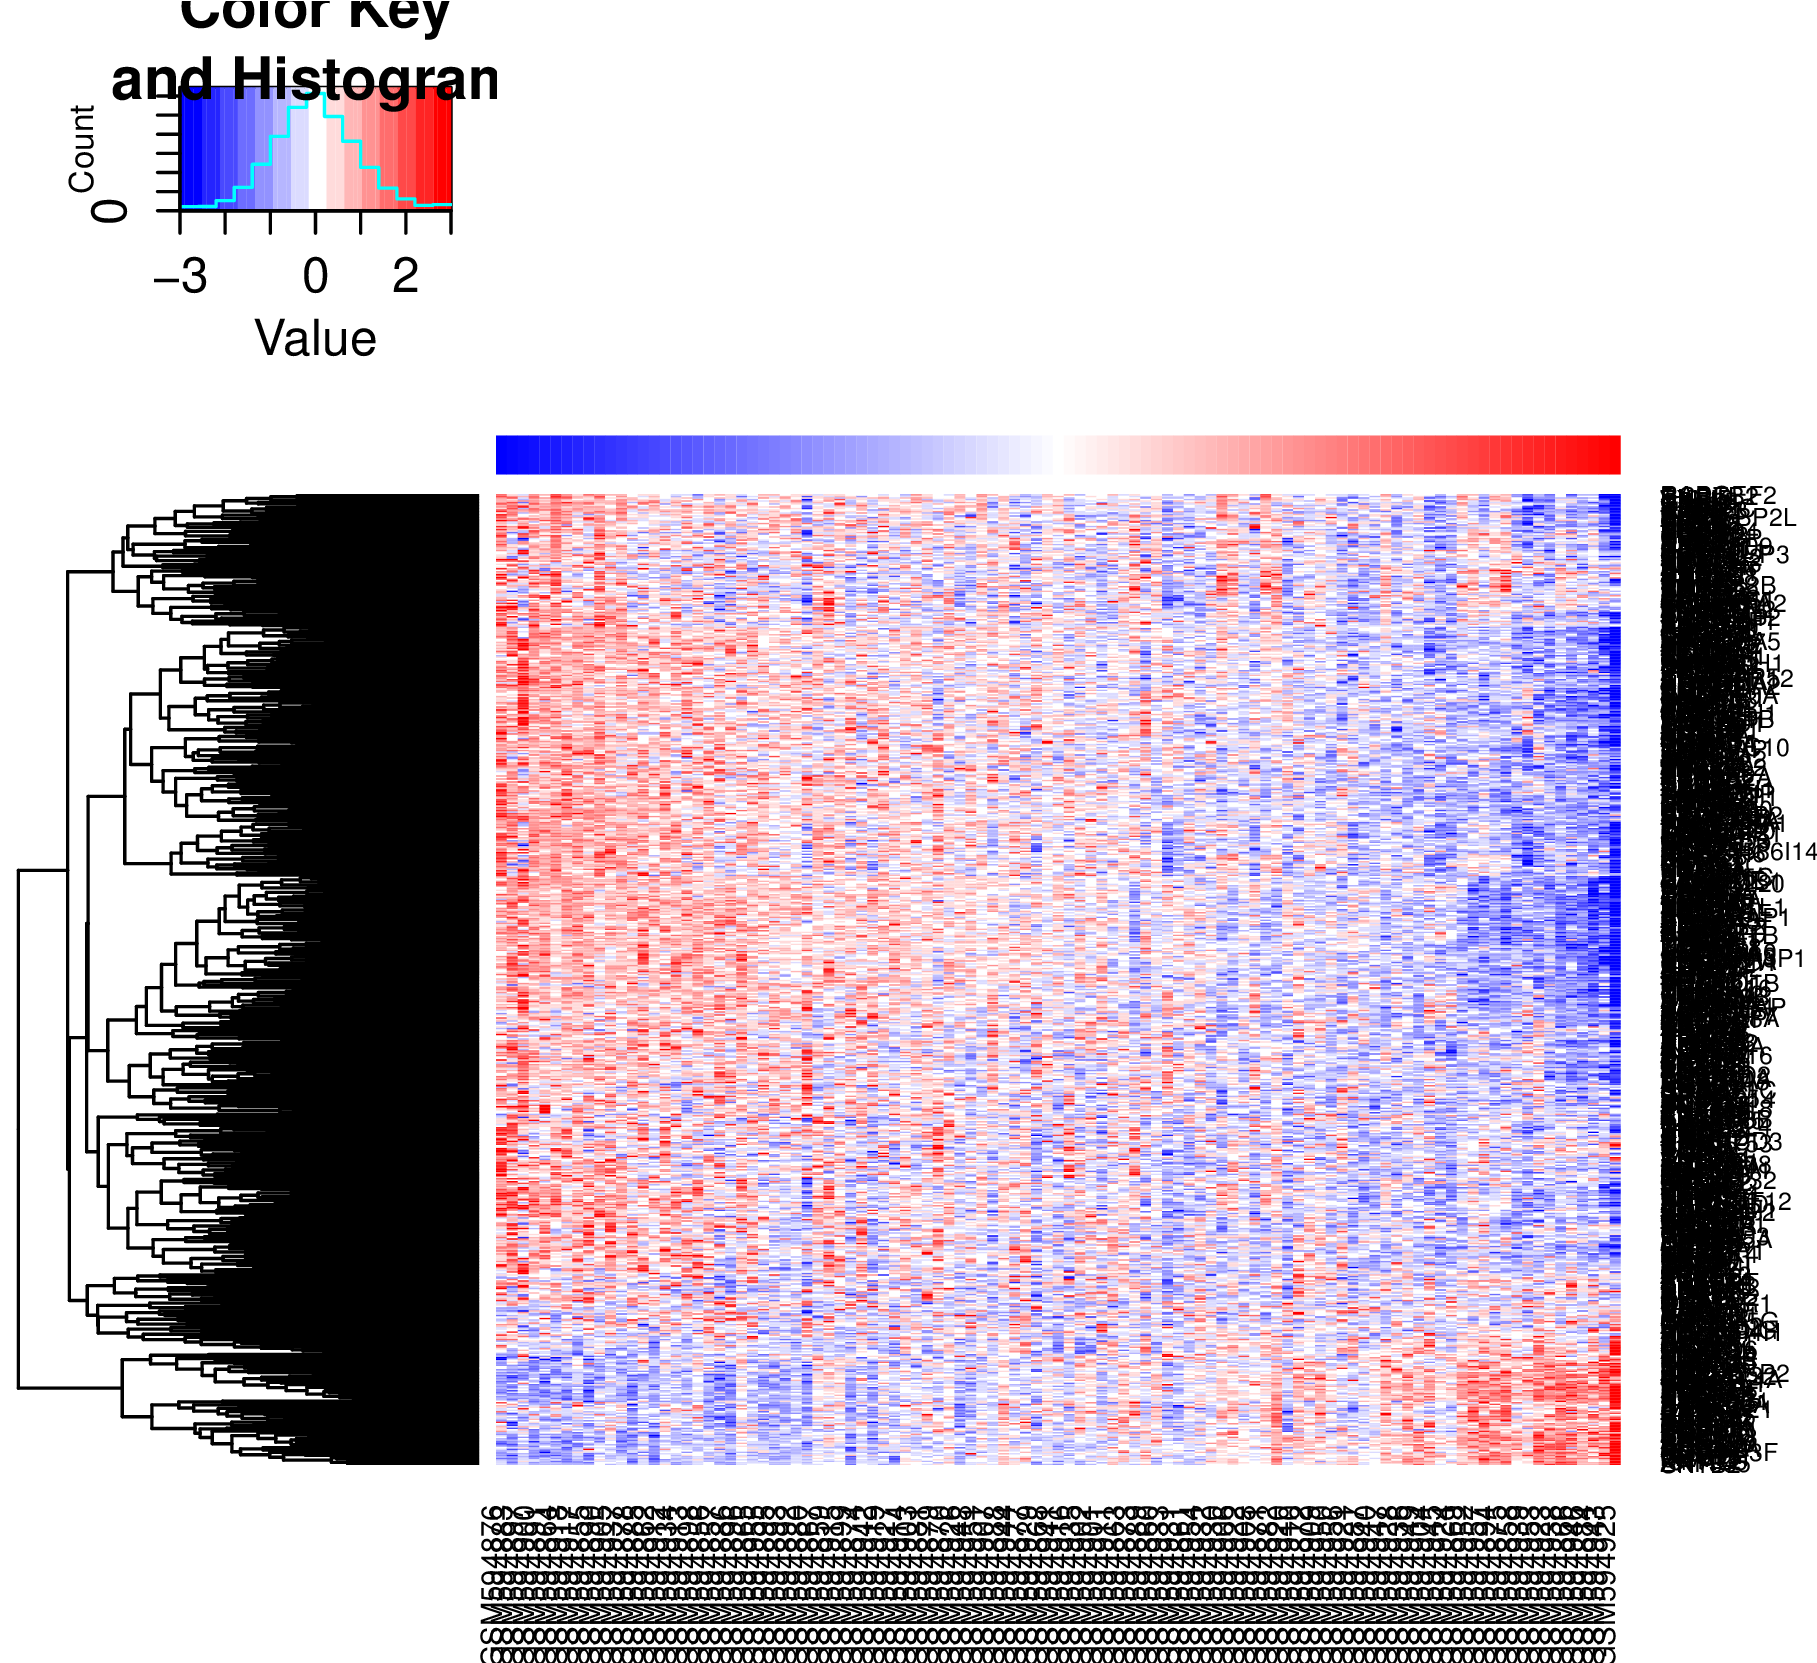
\includegraphics[width=0.45\linewidth]{results1/crmeta_original}
	\hfill
	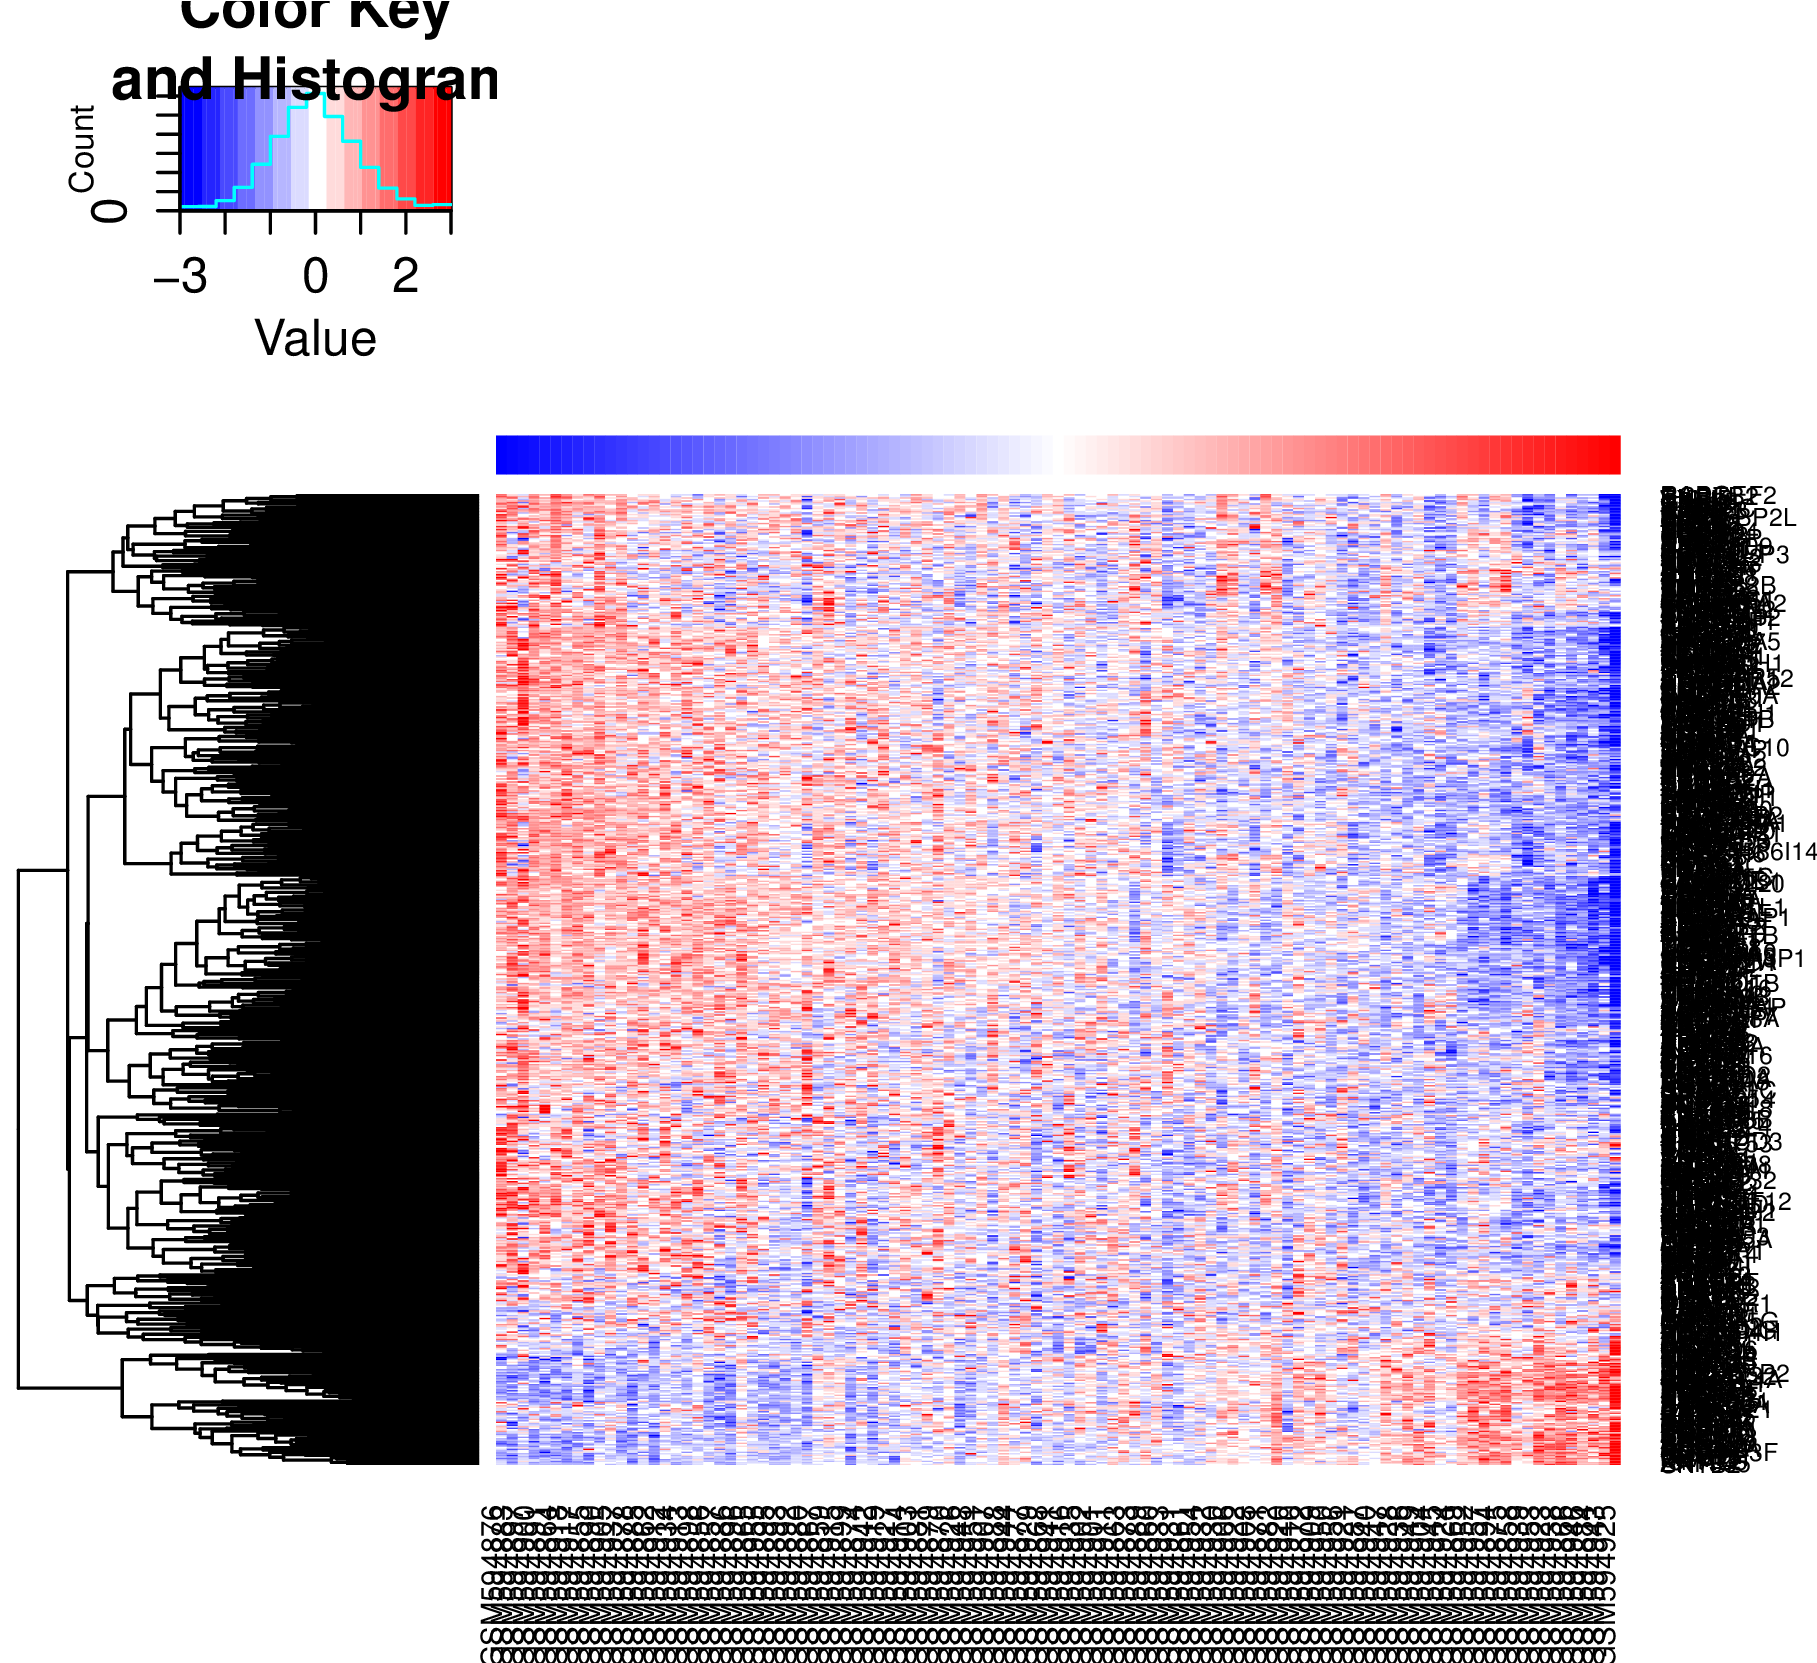
\includegraphics[width=0.45\linewidth]{results1/crmeta_original}
	\caption[Creighton metagene and \acrshort{icgc} cancer data]{(insert ICGC heatmaps)}
	\label{fig:crmetaicgc1}
\end{figure}

\begin{figure}[htp!]
	\centering
	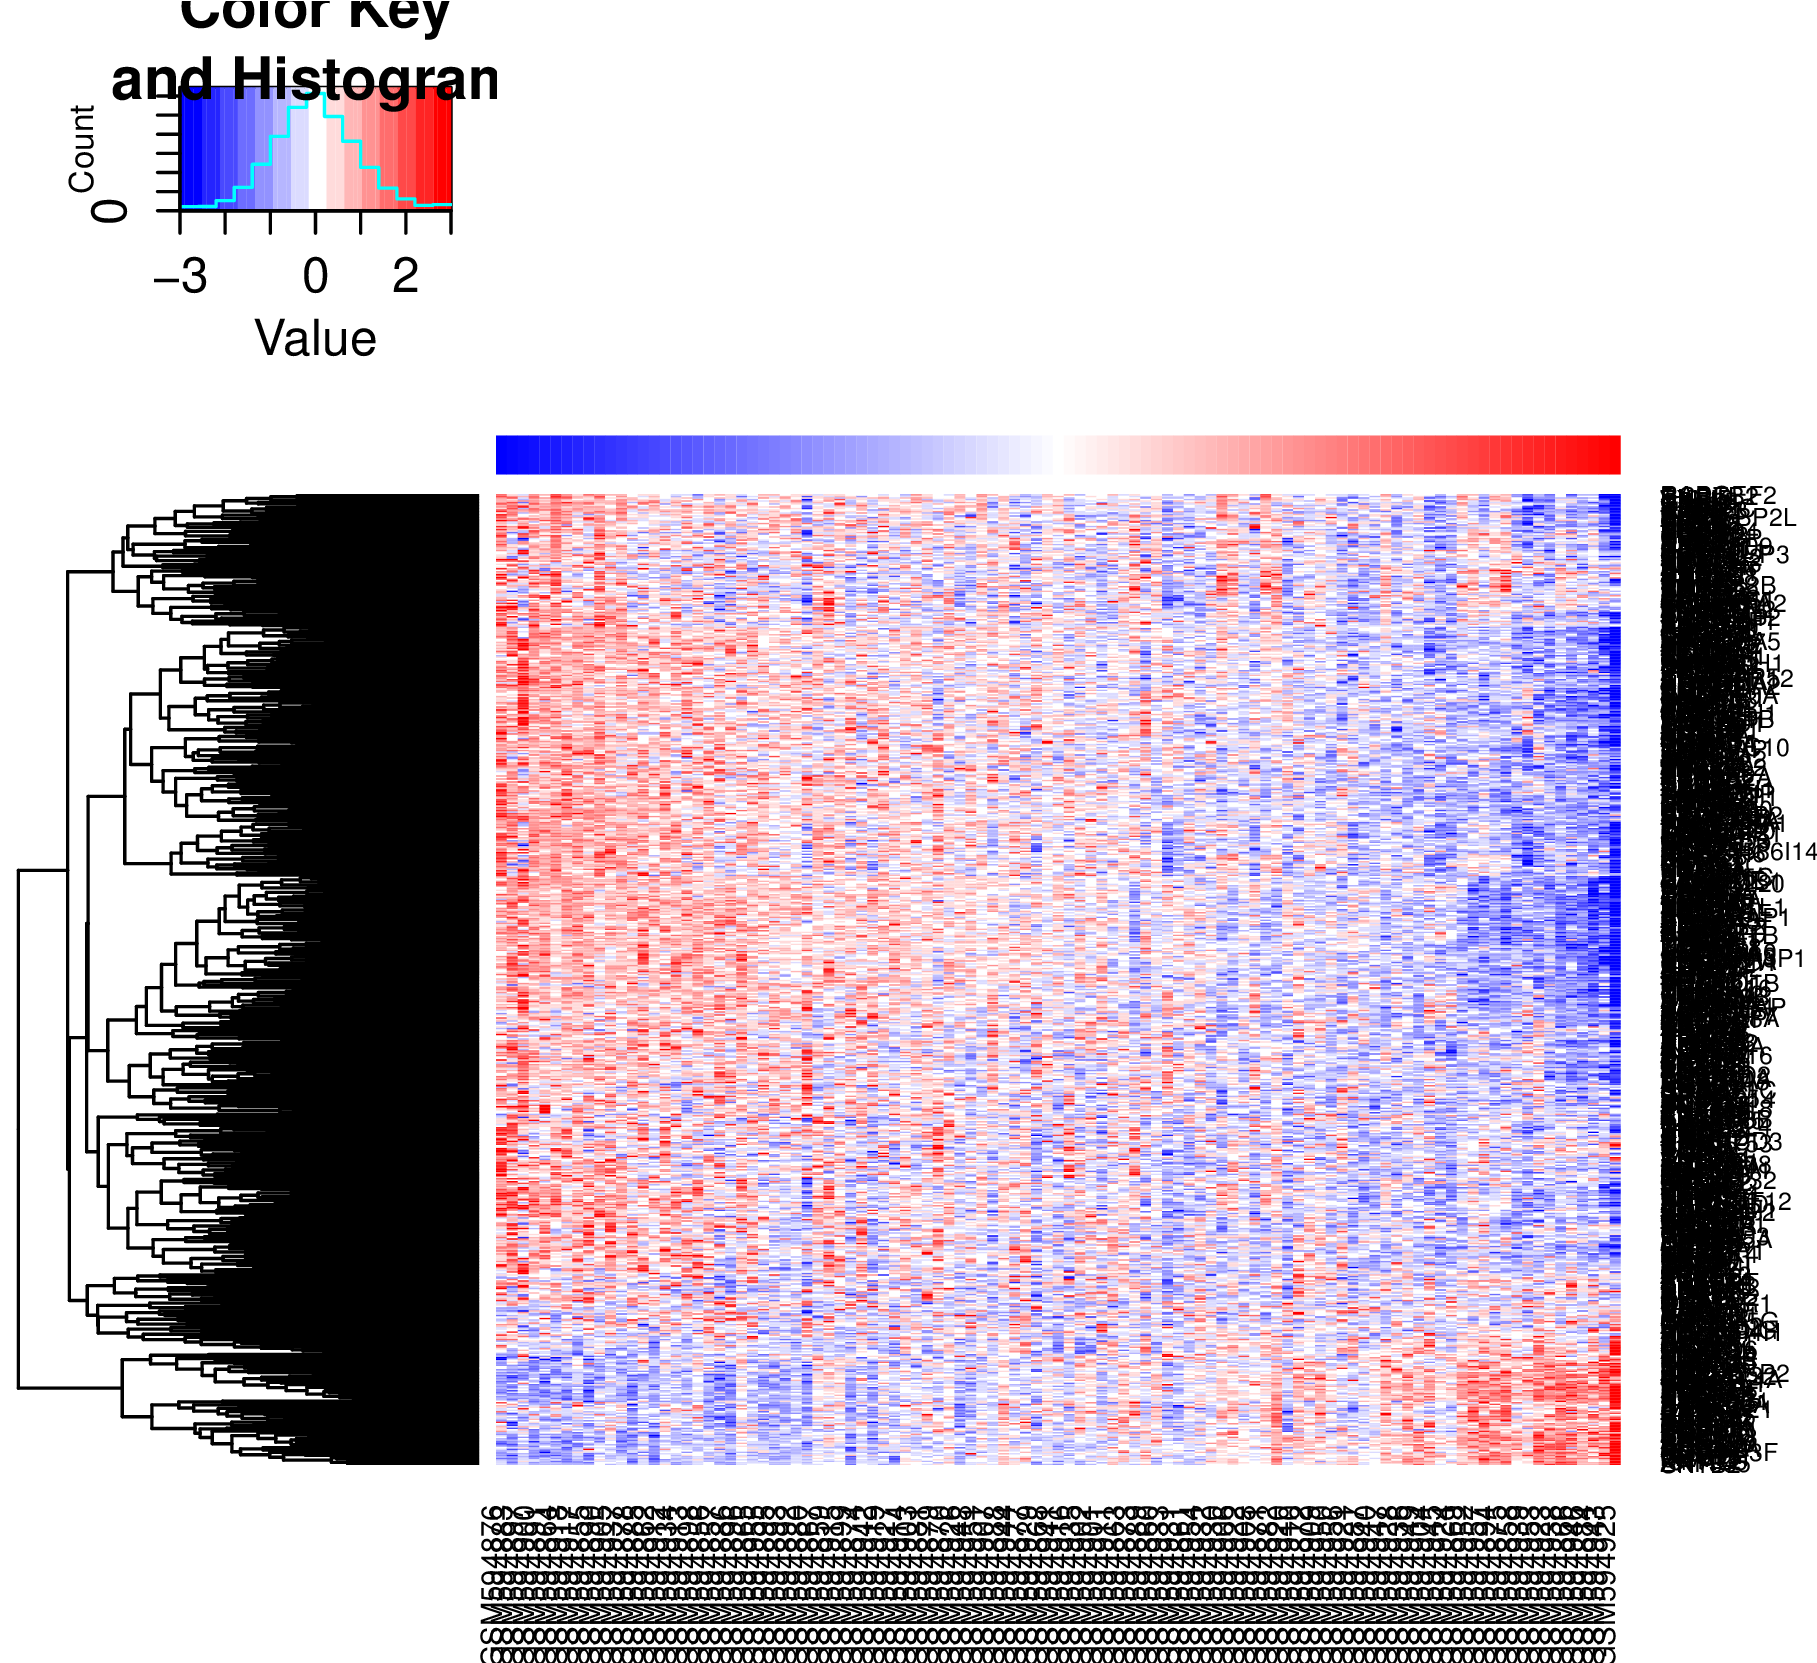
\includegraphics[width=0.45\linewidth]{results1/crmeta_original}
	\hfill
	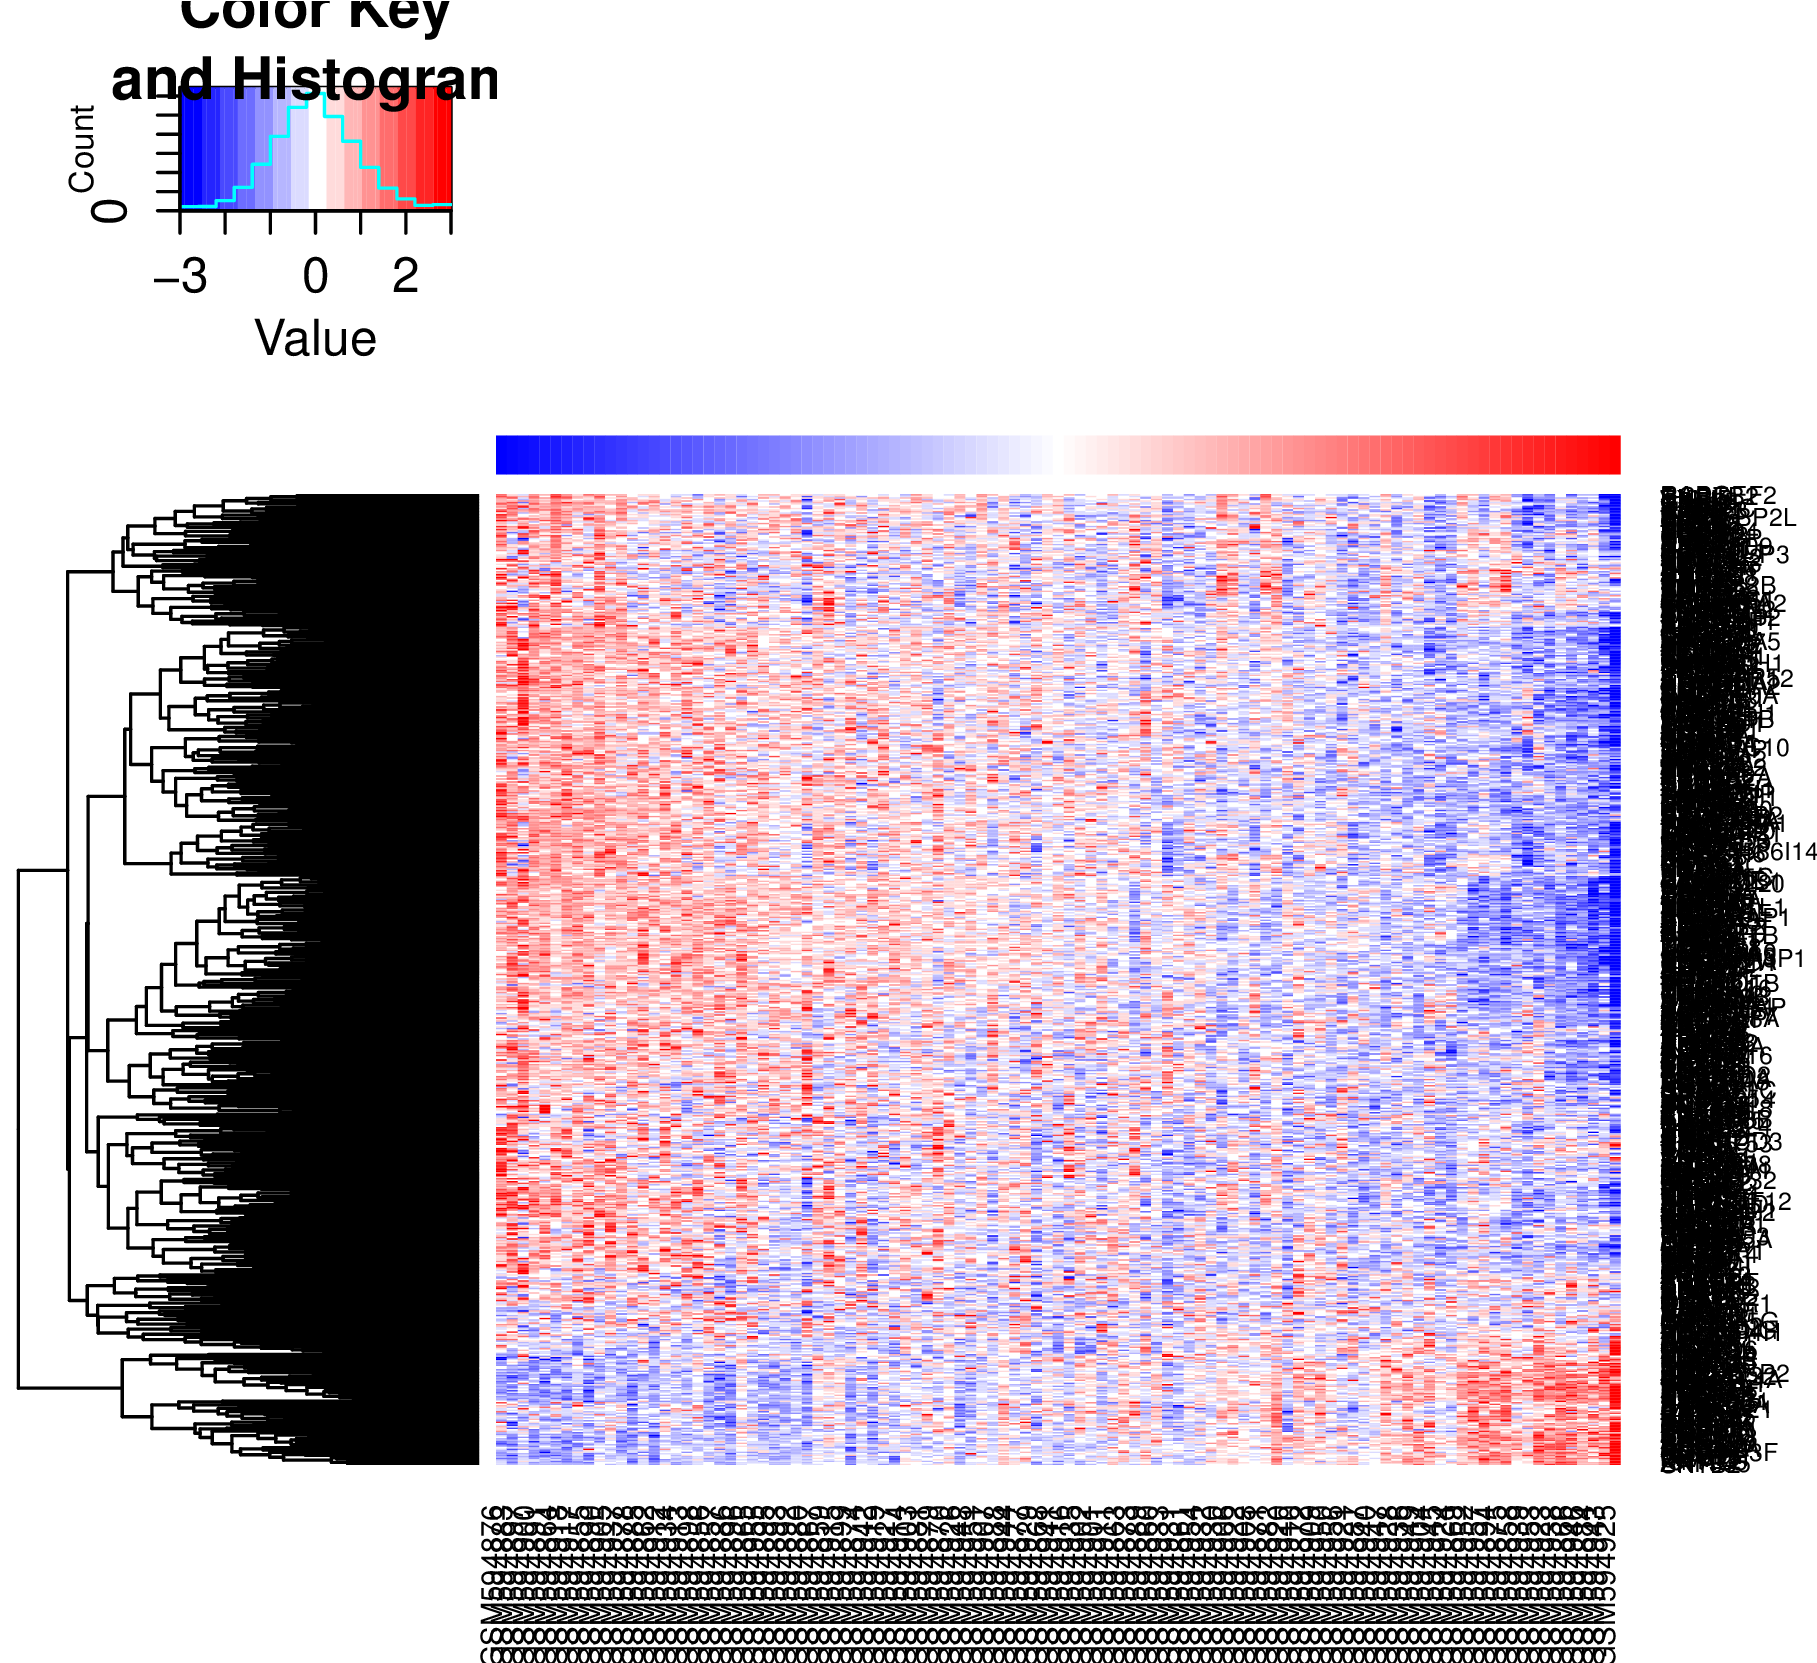
\includegraphics[width=0.45\linewidth]{results1/crmeta_original}
	\caption[Creighton metagene and sample \gls{bmi}/\gls{bmi} status in \acrshort{icgc} data]{(insert figure of box plot and scatter plot for ICGC data)}
	\label{fig:crmetaboxicgc1}
\end{figure}

As before, association of the obesity metagene with the sample \gls{bmi} and \gls{bmi} status was checked in their respective cancer data set (\cref{fig:crmetaboxicgc1}).
In contrast to the strong association of the obesity metagene with sample \gls{bmi} and \gls{bmi} status in Creighton's data, the obesity metagene taken from the \gls{icgc} cancer data did not significantly associate with the sample \gls{bmi} or \gls{bmi} status in any of the \gls{icgc} cancer data.

There could be several reasons for the apparent lack of association of the metagene with the sample \gls{bmi} or \gls{bmi} status.
First, transformation matrix was derived from Creighton's microarray data, but the \gls{icgc} cancer data were \gls{rnaseq} data.
Though the log$_{10}$ normalisation and standardisation of the data was the most appropriate adjustment to be made to the \gls{rnaseq} data, this adjustment may not be equivalent to the \gls{rma} normalisation method that was used on the microarray data.
Secondly, none of the \gls{icgc} cancer was from breast as in Creighton's data.
Since the obesity associated signature was identified in breast cancer data, the signature may be specific to breast cancer and may not be suitable in other cancer types.
\\

\noindent
To check whether the metagene was specific to breast cancer microarray data, the same transformation matrix was applied to Print's breast cancer microarray data.
Print's data was normalised with \gls{rma} method as described in \cref{ssub:microarray_data}, and the transformation matrix was applied to the normalised data to obtain the metagene.
The metagene was again compared with the gene expression of the samples with a heatmap (\cref{fig:crmetaprint1}), and the association of the metagene with the sample \gls{bmi} and \gls{bmi} status was examined with box and scatter plots (\cref{fig:crmetaboxprint1}).

\begin{figure}[htp!]
	\centering
	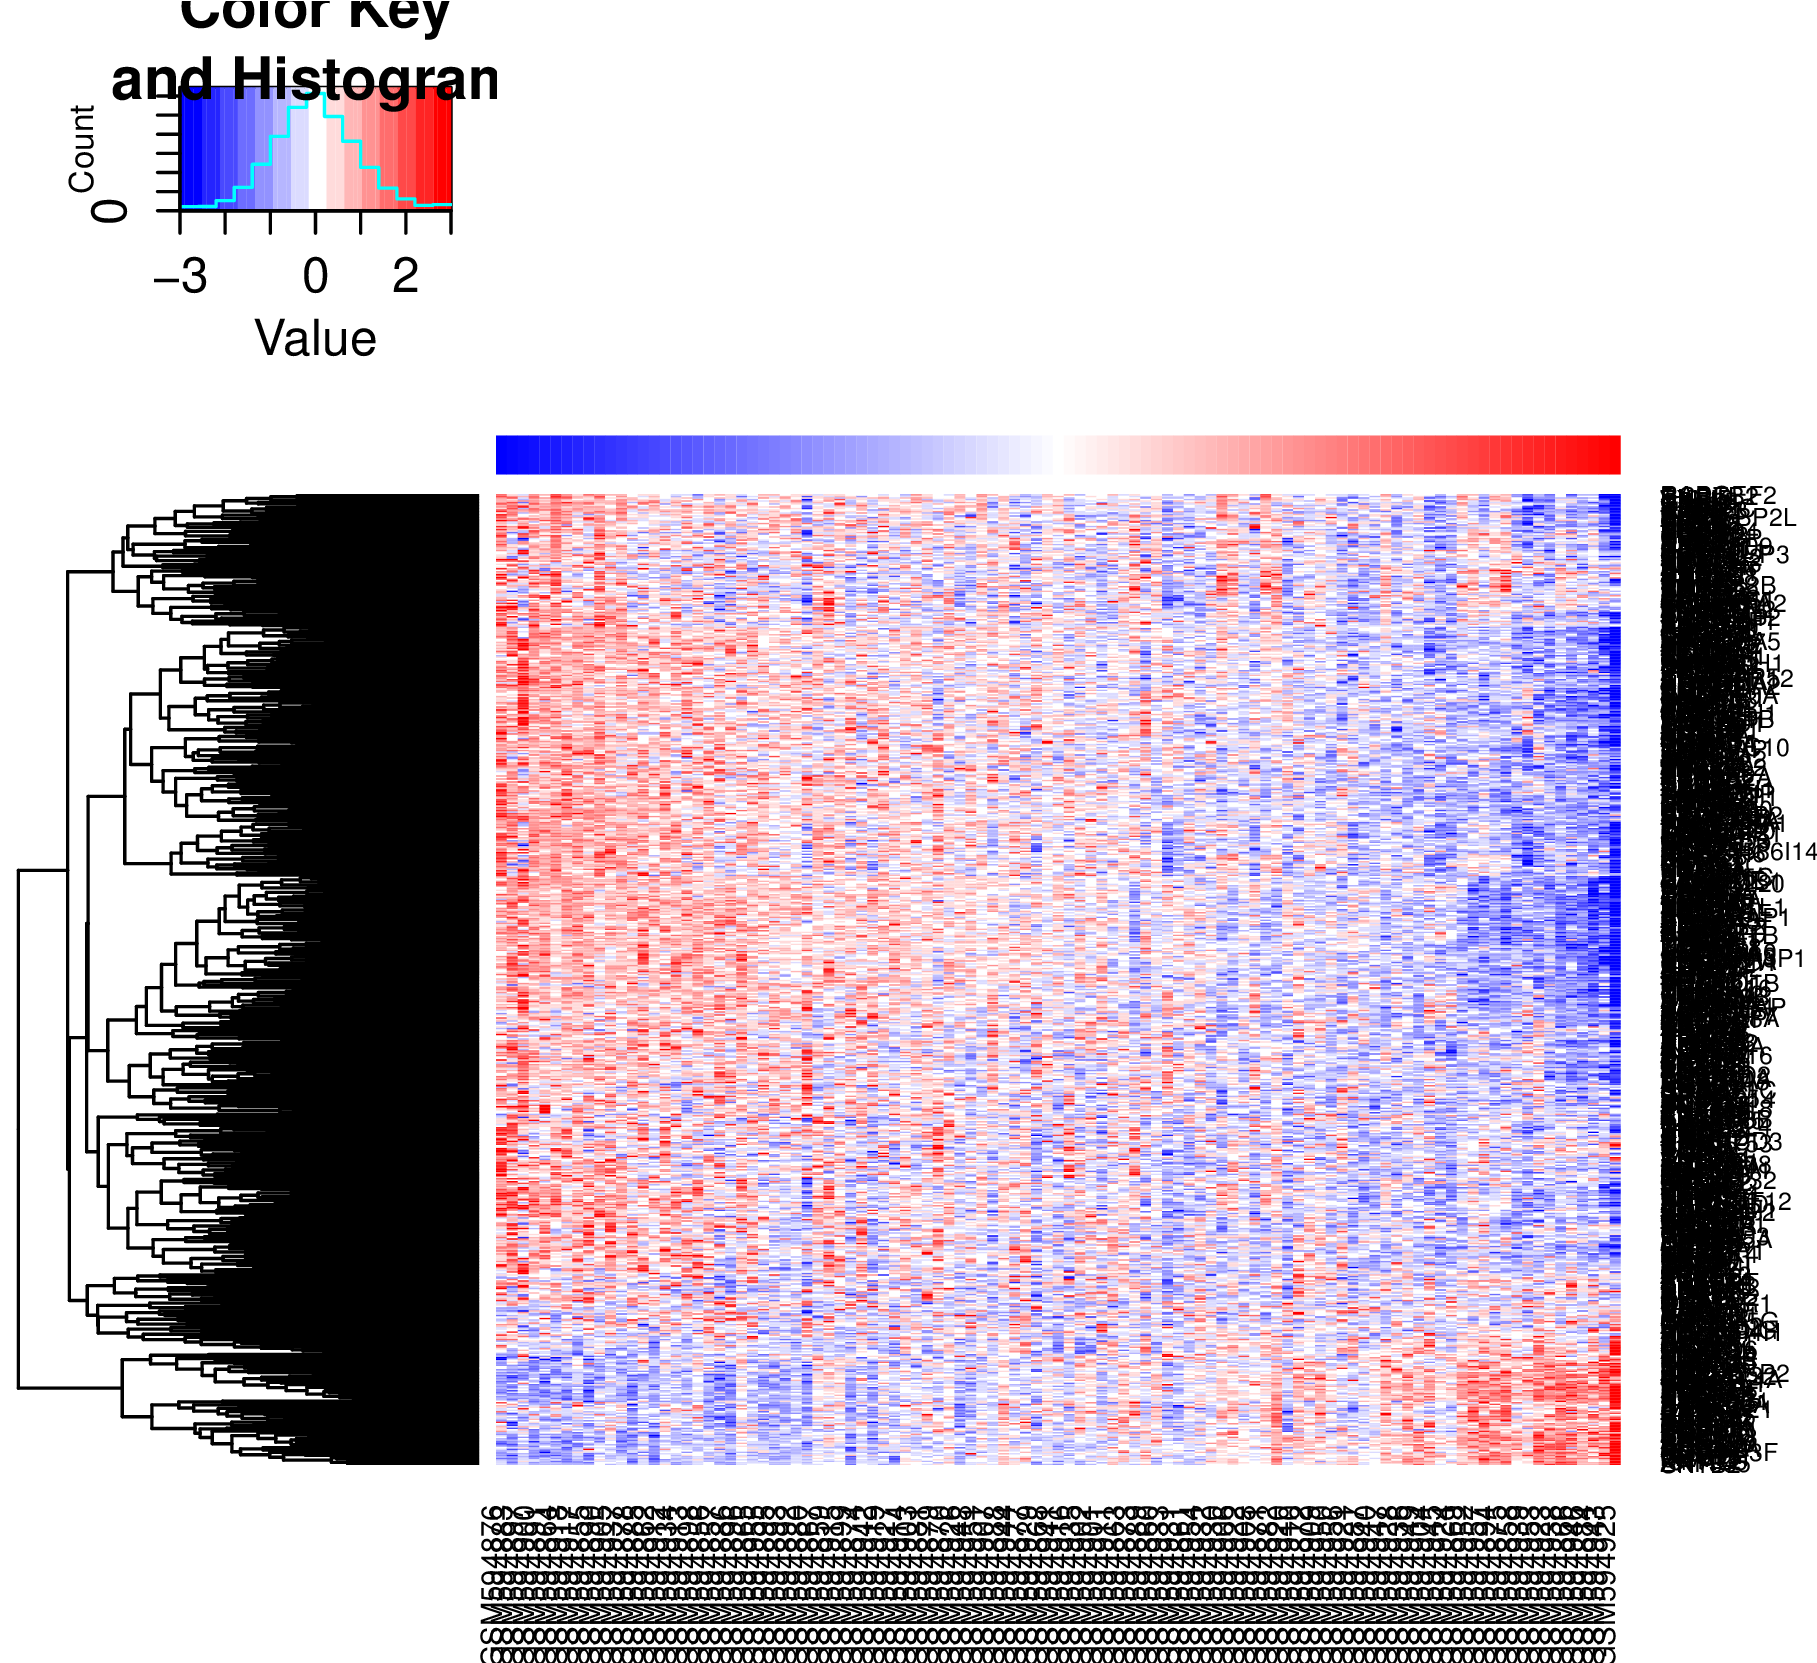
\includegraphics[width=0.45\linewidth]{results1/crmeta_original}
	\hfill
	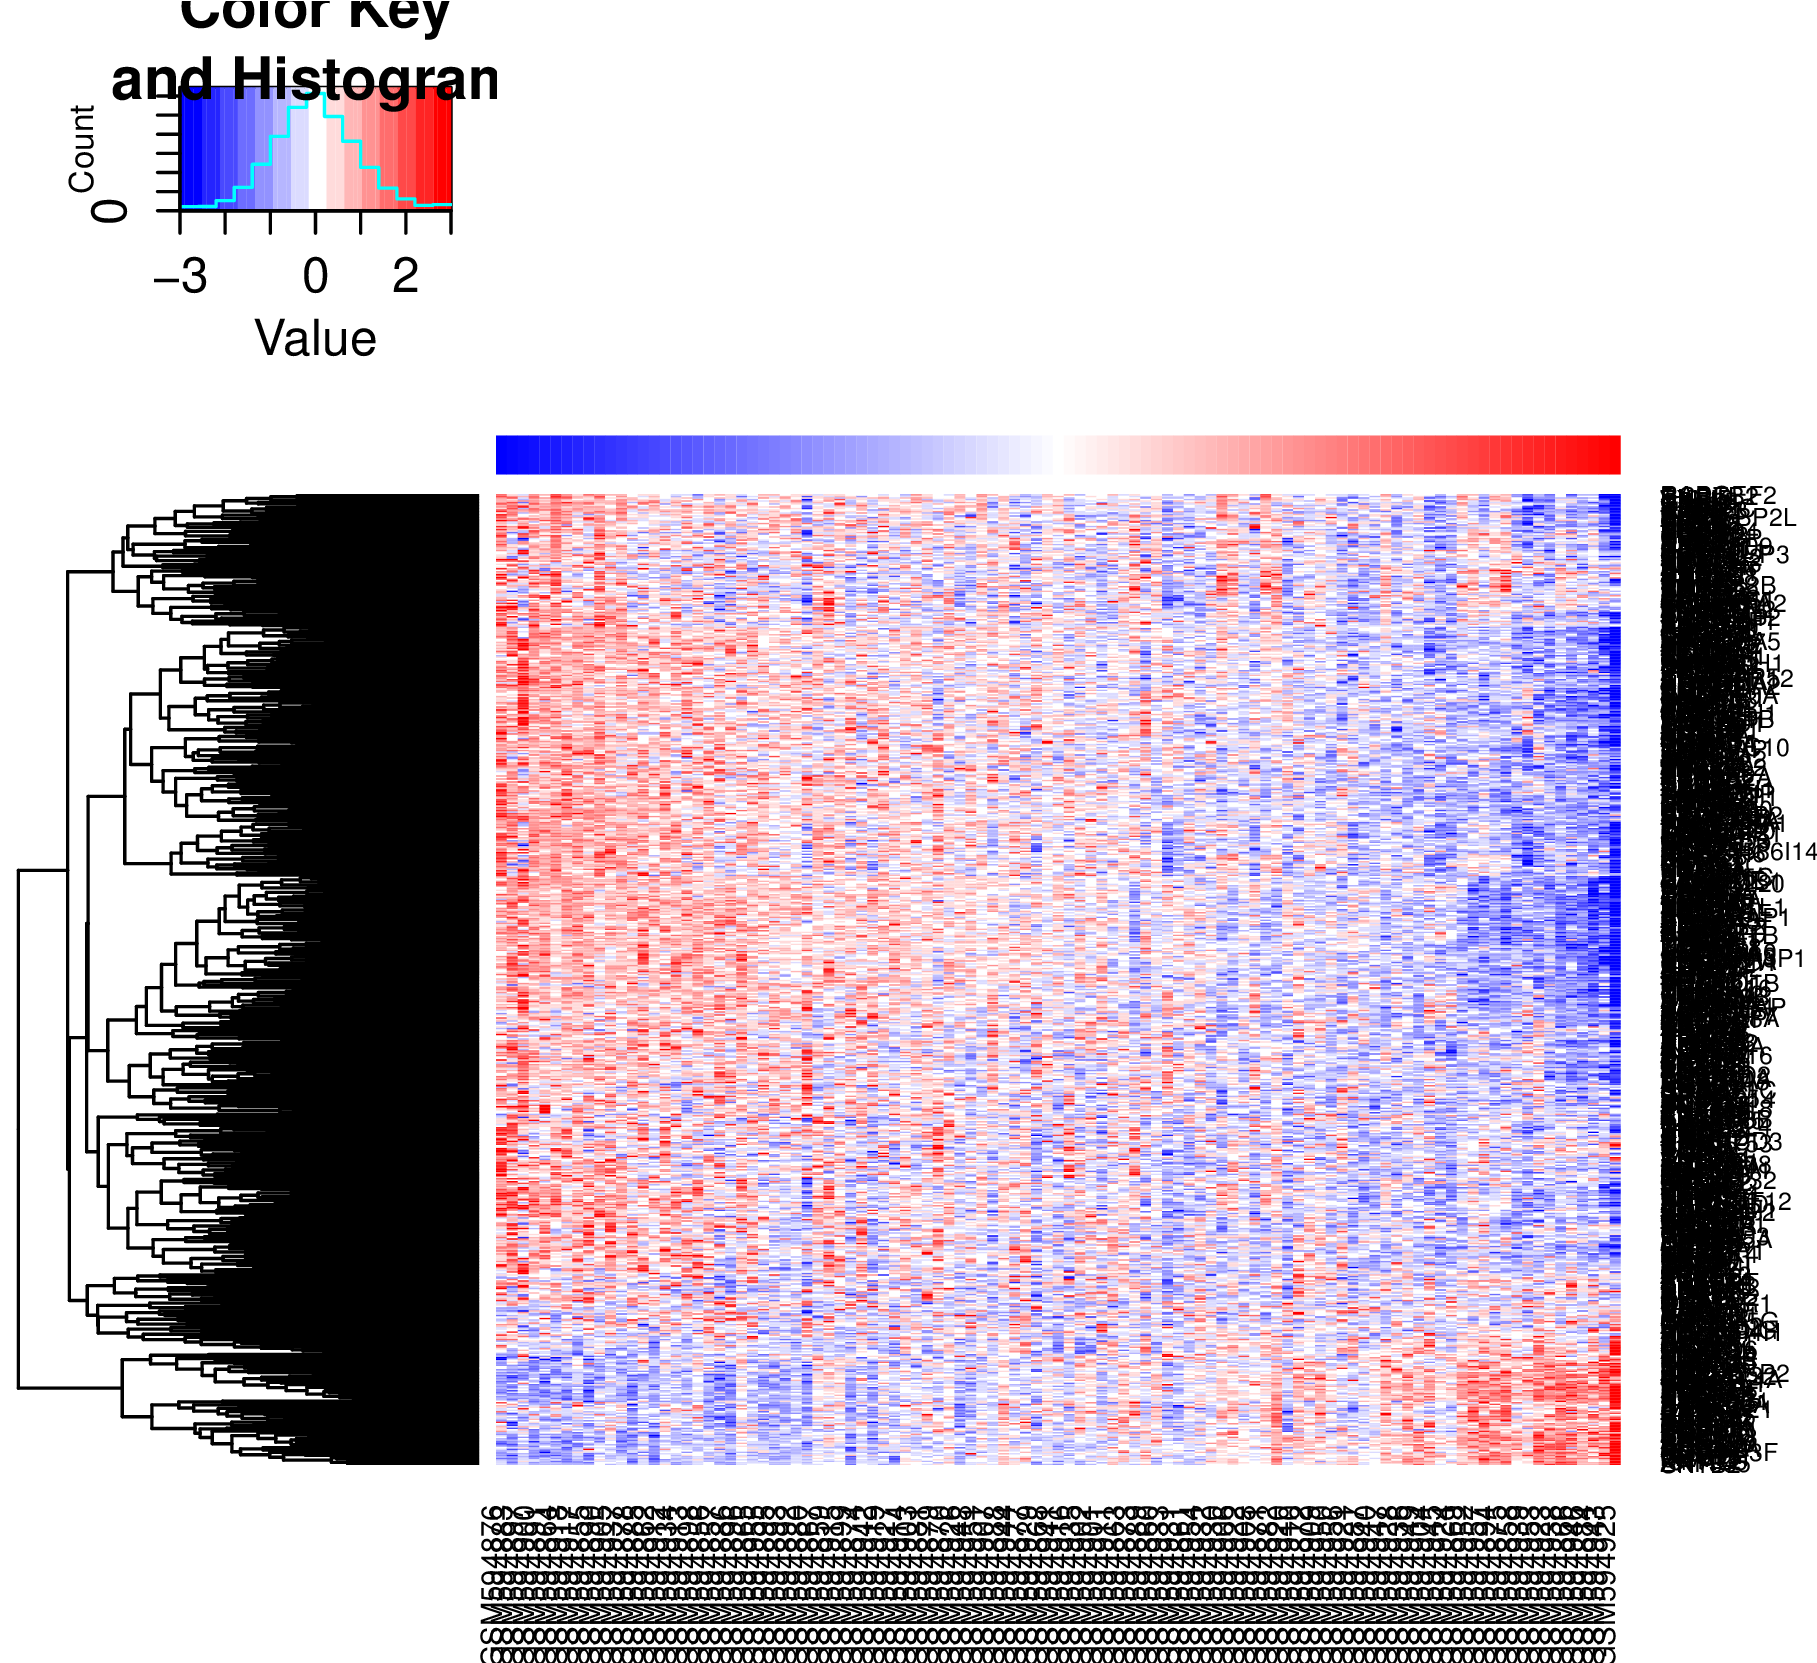
\includegraphics[width=0.45\linewidth]{results1/crmeta_original}
	\caption[Creighton metagene and Print's cancer data]{(insert Print heatmaps)}
	\label{fig:crmetaprint1}
\end{figure}

\begin{figure}[htp!]
	\centering
	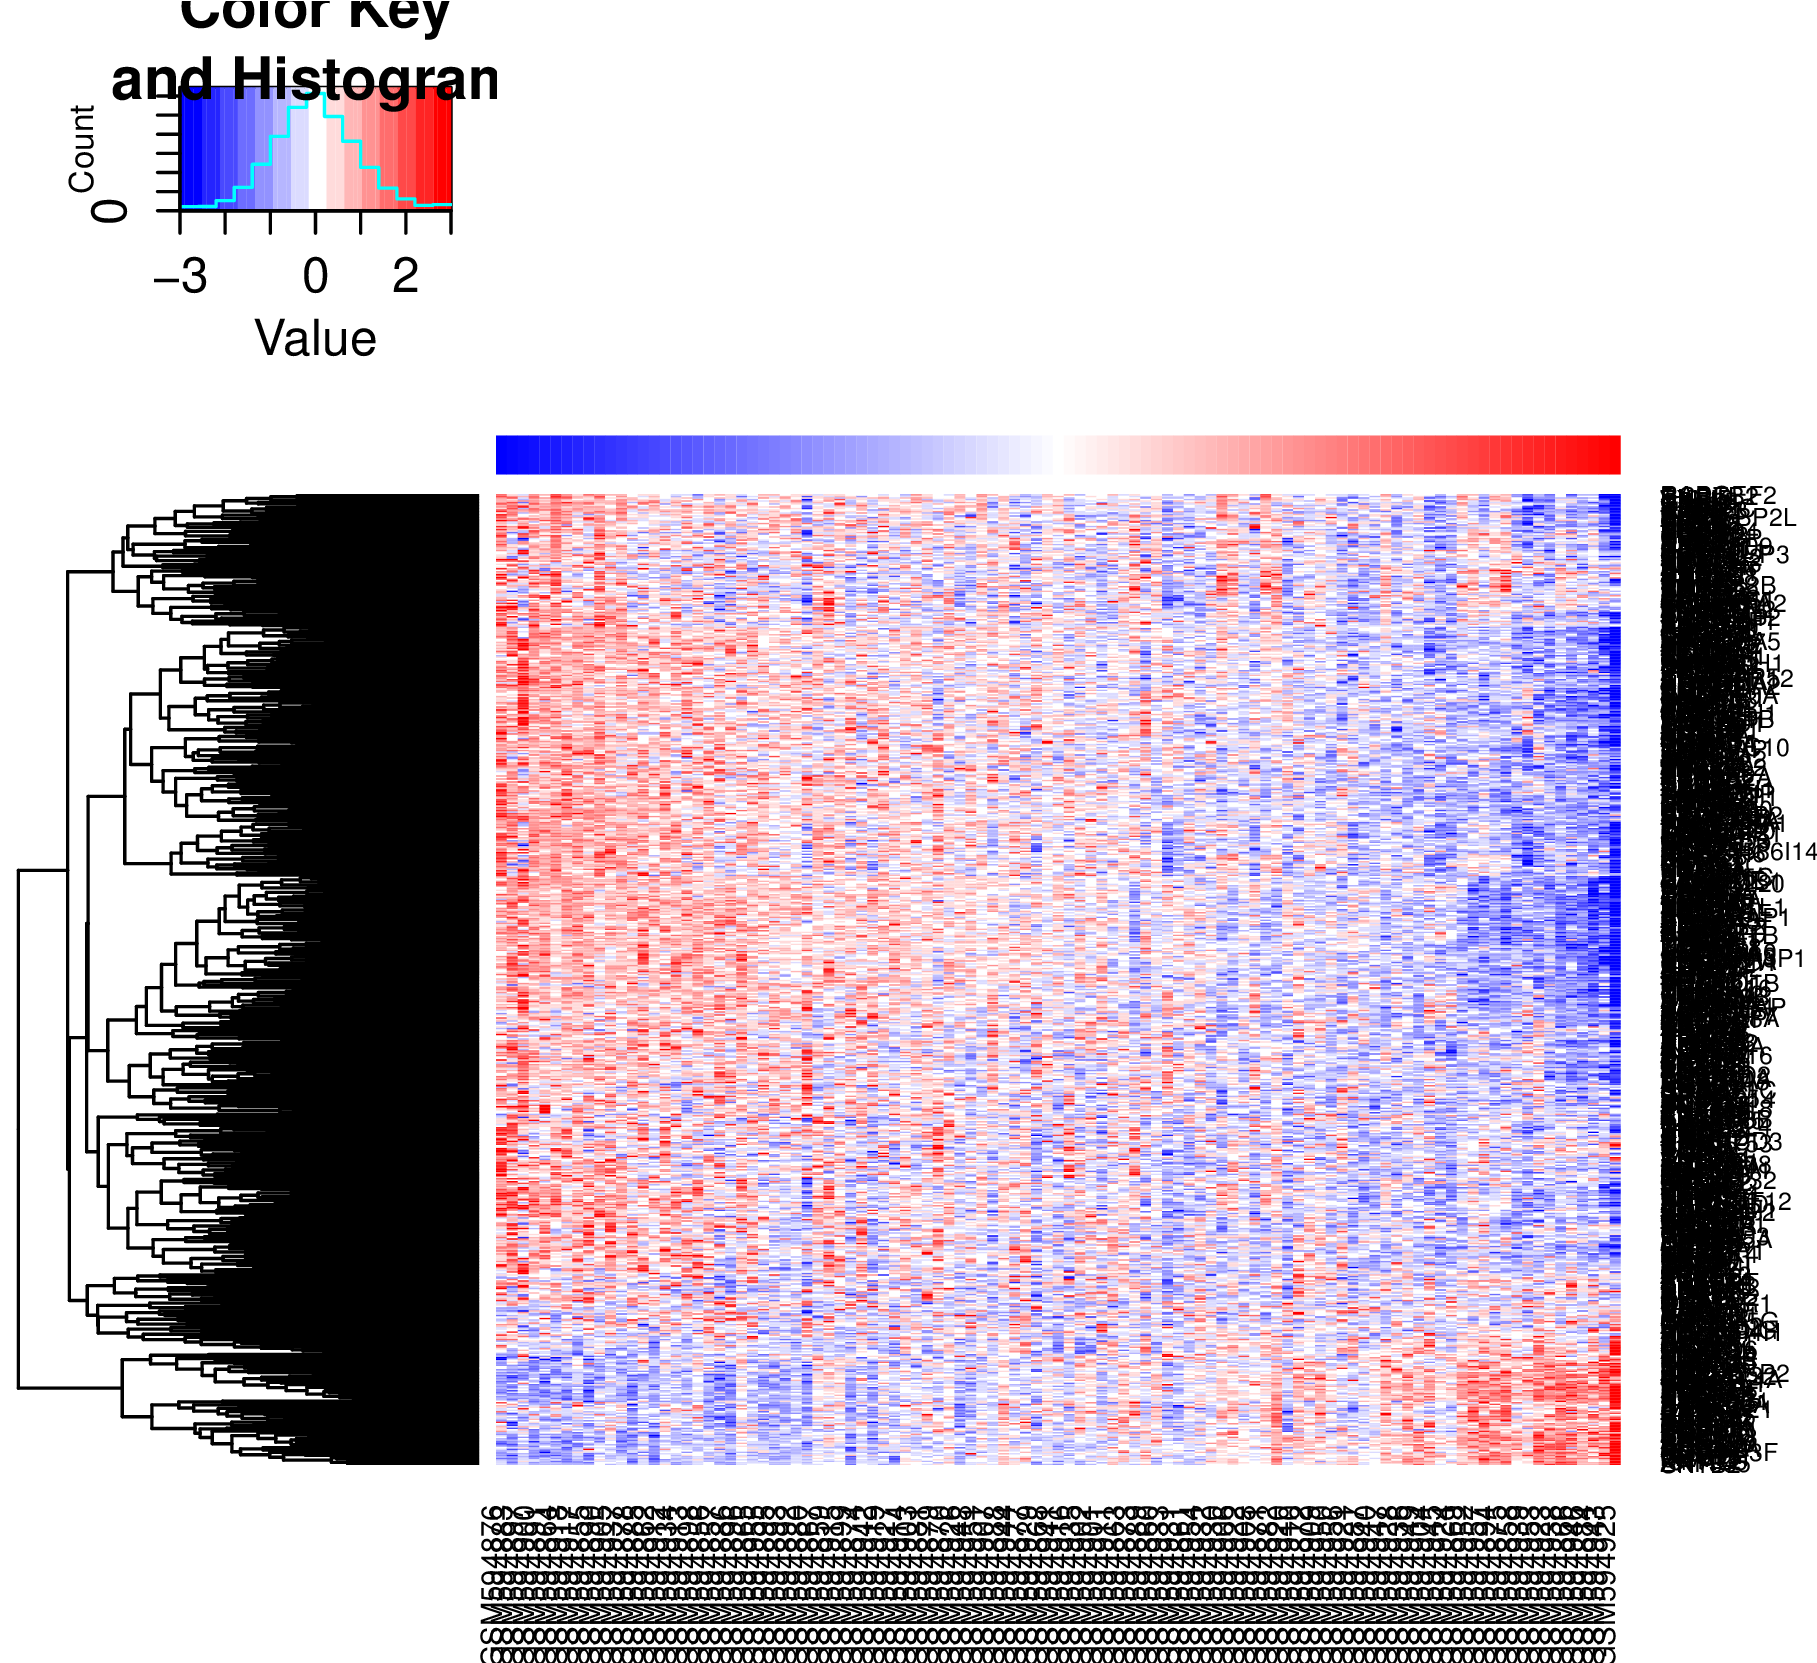
\includegraphics[width=0.45\linewidth]{results1/crmeta_original}
	\hfill
	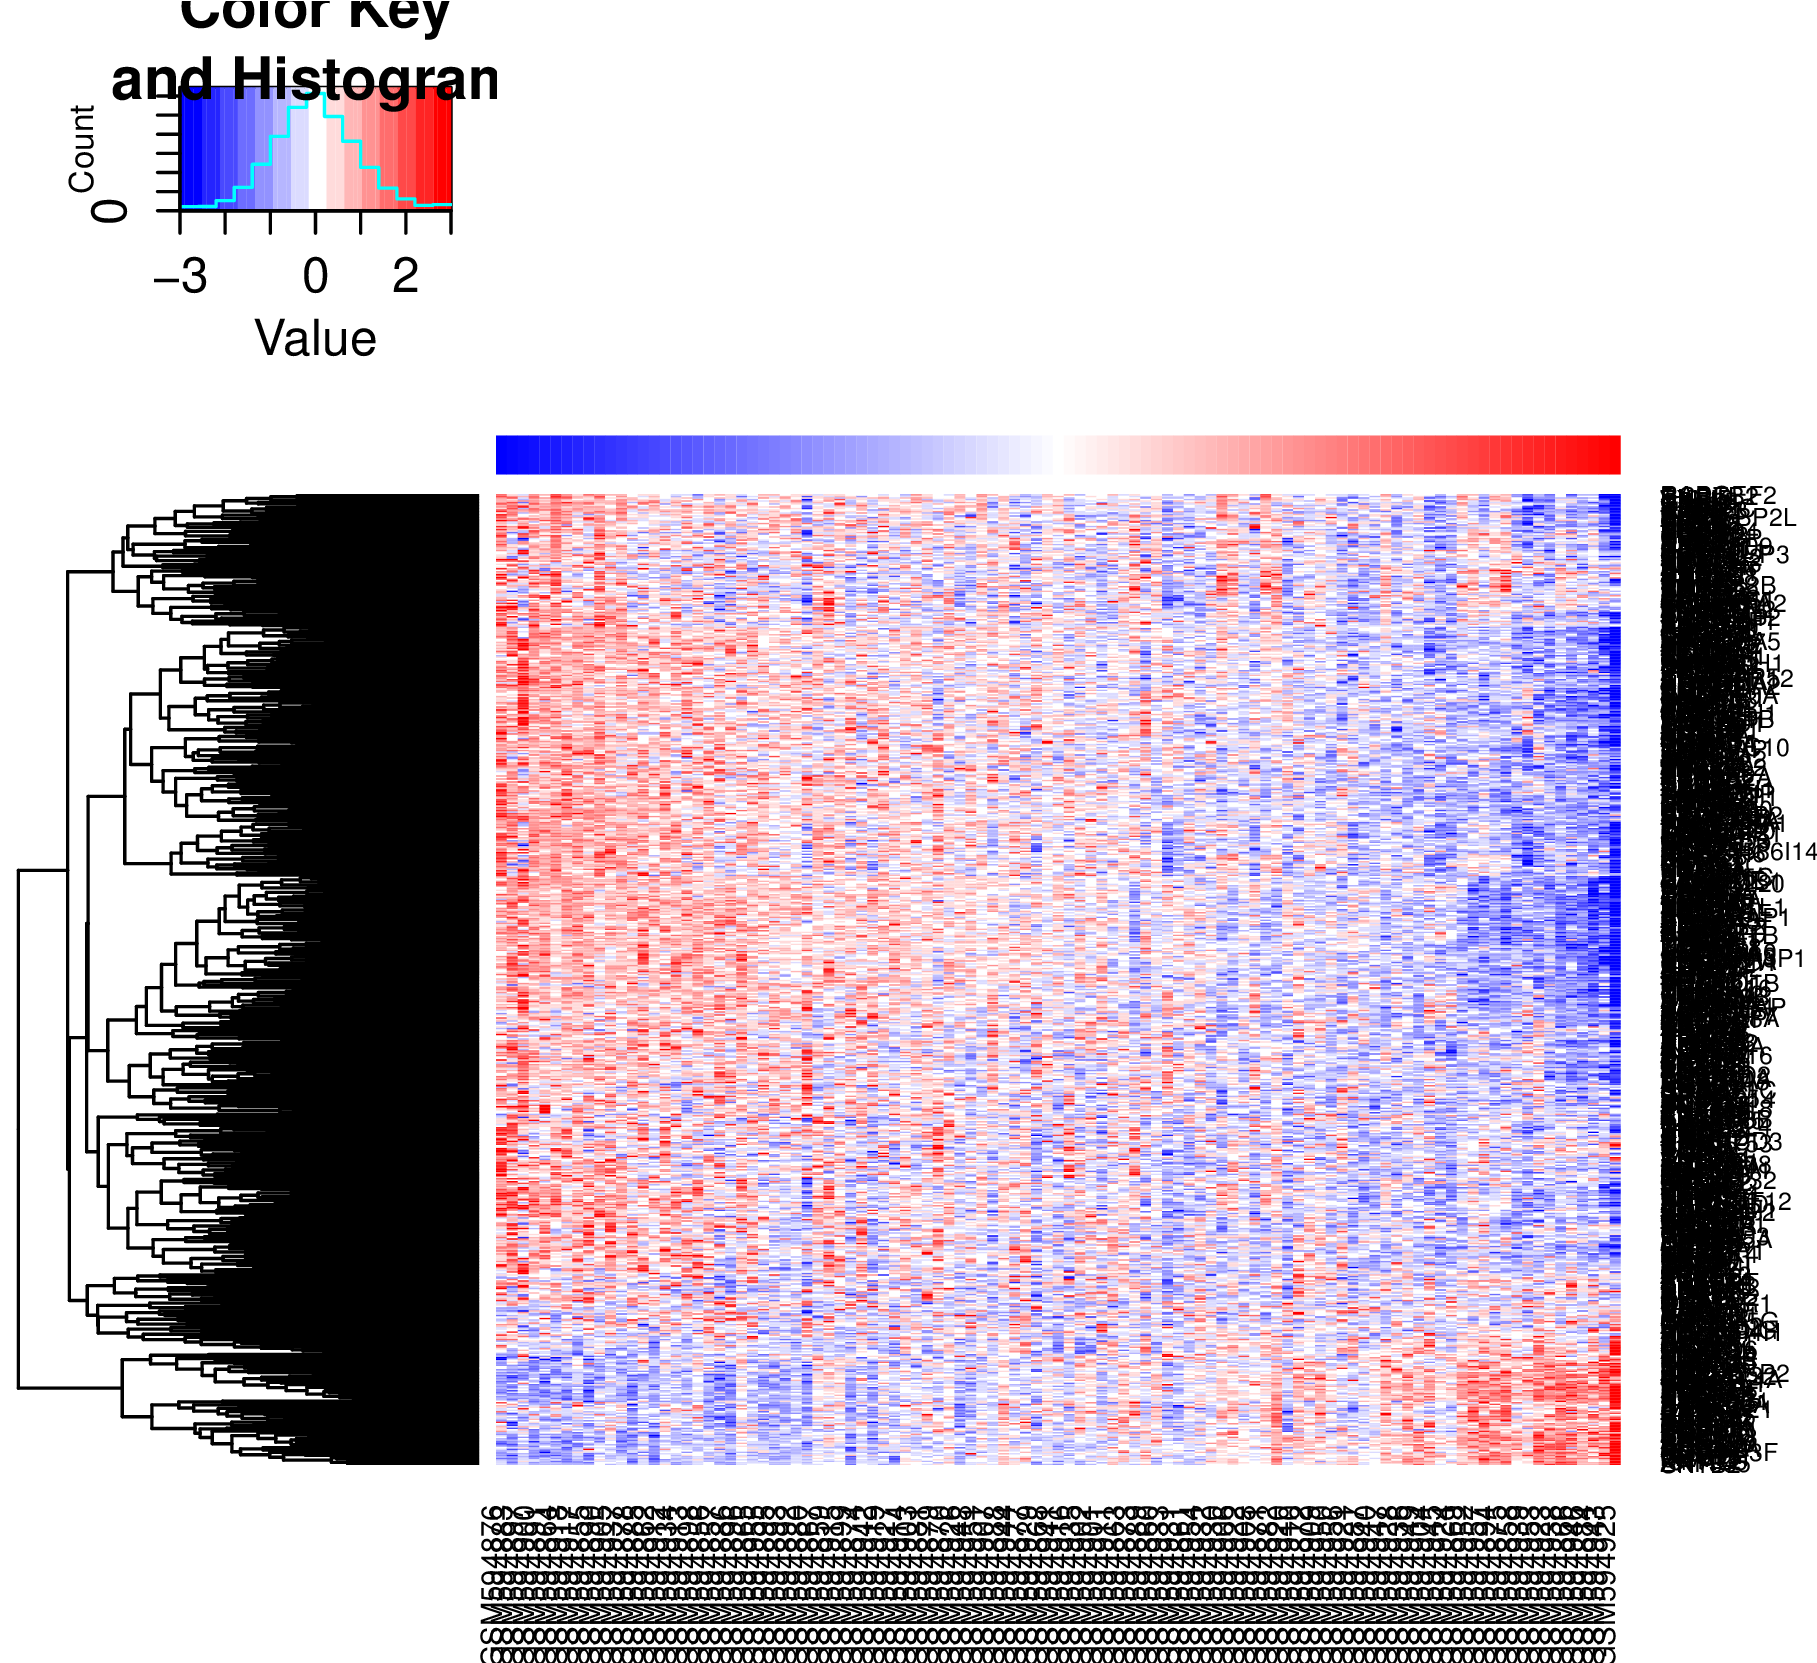
\includegraphics[width=0.45\linewidth]{results1/crmeta_original}
	\caption[Creighton metagene and sample \gls{bmi}/\gls{bmi} status in Print's data]{(insert figure of box plot and scatter plot for Print data)}
	\label{fig:crmetaboxprint1}
\end{figure}

The obesity metagene managed to reflect the overall gene expression of the samples in Print's data.
However, like in \gls{icgc} cancer data, the obesity metagene scores did not significantly associate with the sample \gls{bmi} or \gls{bmi} status.
These results confirmed that the lack of association of the obesity metagene from Creighton's data was not due to the technology in which the data was gathered (mcroarray or \gls{rnaseq}), nor the type of cancer in which the transformation matrix was applied to.

All together, all of these results suggest that the obesity metagene identified in the study conducted by \citet{Creighton2012} associated with sample \gls{bmi} and \gls{bmi} status in Creighton's data, but did not transfer well in other cancer data sets.
The lack of association with \gls{bmi} was not due to the type of technology platform in which the data was gathered, as neither the \gls{icgc} \gls{rnaseq} data nor Print's microarray data did not show significant association with the obesity metagene.
Furthermore, Creighton's metagene was not dependent on the cancer type since the obesity associated genetic signature did not show significant association in neither the \gls{icgc} cancer data nor in Print's breast cancer data.

One possible reason why Creighton's obesity metagene did not show significant association with other data sets could be because the genetic signature was in fact not an obesity specific signature, but a signature that detected another clinical variable.
Another reason for this apparent lack of association could be that the genetic signature was too specific to the data and was not a broad obesity associated genetic signature, but an obesity associated signature specifically for Creighton's data set.

\section{Obesity associated genetic signature from \citet{Fuentes-Mattei2014} study}
\label{sec:fm_obesity_metagene}

Since Creighton's obesity associated genetic signature was not associated with sample \gls{bmi} or \gls{bmi} status in other data sets, Fuentes-Mattei's (FM) obesity associated genetic signature was examined to see whether FM's obesity metagene associated with sample \gls{bmi} or \gls{bmi} status.
Since FM's data set did not have sample \gls{bmi} information, FM's obesity metagene was not able to be compared with the sample \gls{bmi} or \gls{bmi} status in the original FM's data.
However, the transformation matrix was still applied to other cancer data to see whether FM's obesity metagene associated with sample \gls{bmi}/\gls{bmi} status

Firstly, FM's data was normalised with the \gls{rma} method and \gls{svd} was applied to the normalised data to get the transformation matrix.
The transformation matrix was used to transform the \gls{rma}-normalised Creighton's data to extract FM's obesity metagene scores.
FM's obesity metagene scores were compared with gene expressions and sample \gls{bmi}/\gls{bmi} status in Creighton's data, as shown in \cref{fig:fmmetacr1,fig:fmmetaboxcr1}.
Clearly, like with Creighton's obesity metagene, FM's obesity metagene was reflective of the overall gene expression of the samples, but did not associate with the sample \gls{bmi} or \gls{bmi} status.

\begin{figure}[htp!]
	\centering
	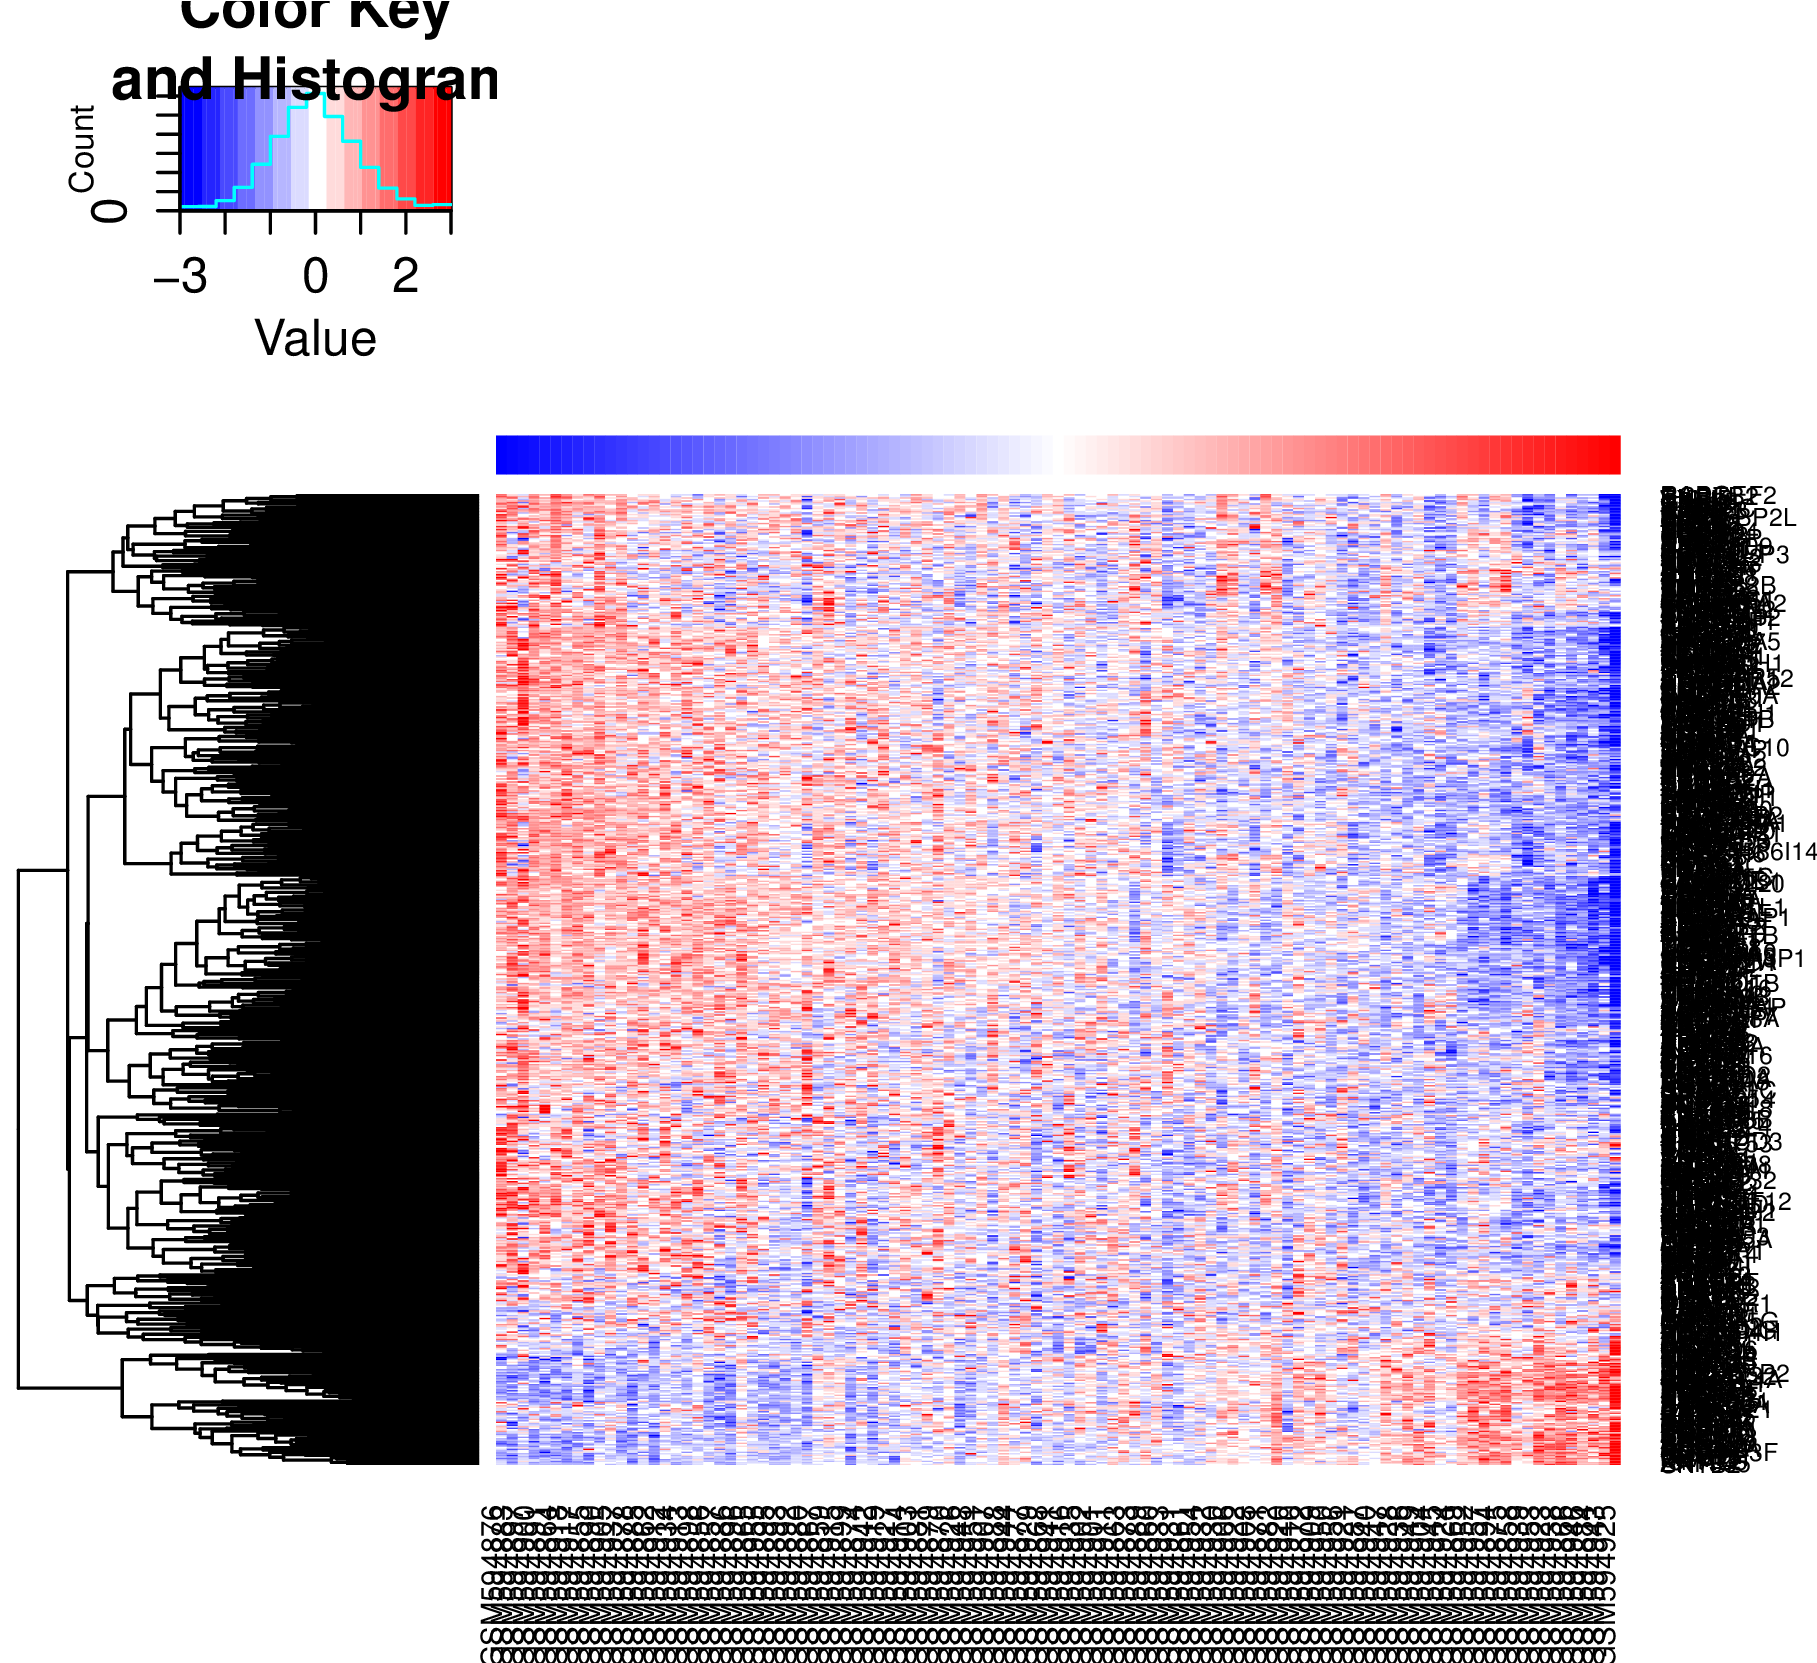
\includegraphics[width=0.45\linewidth]{results1/crmeta_original}
	\hfill
	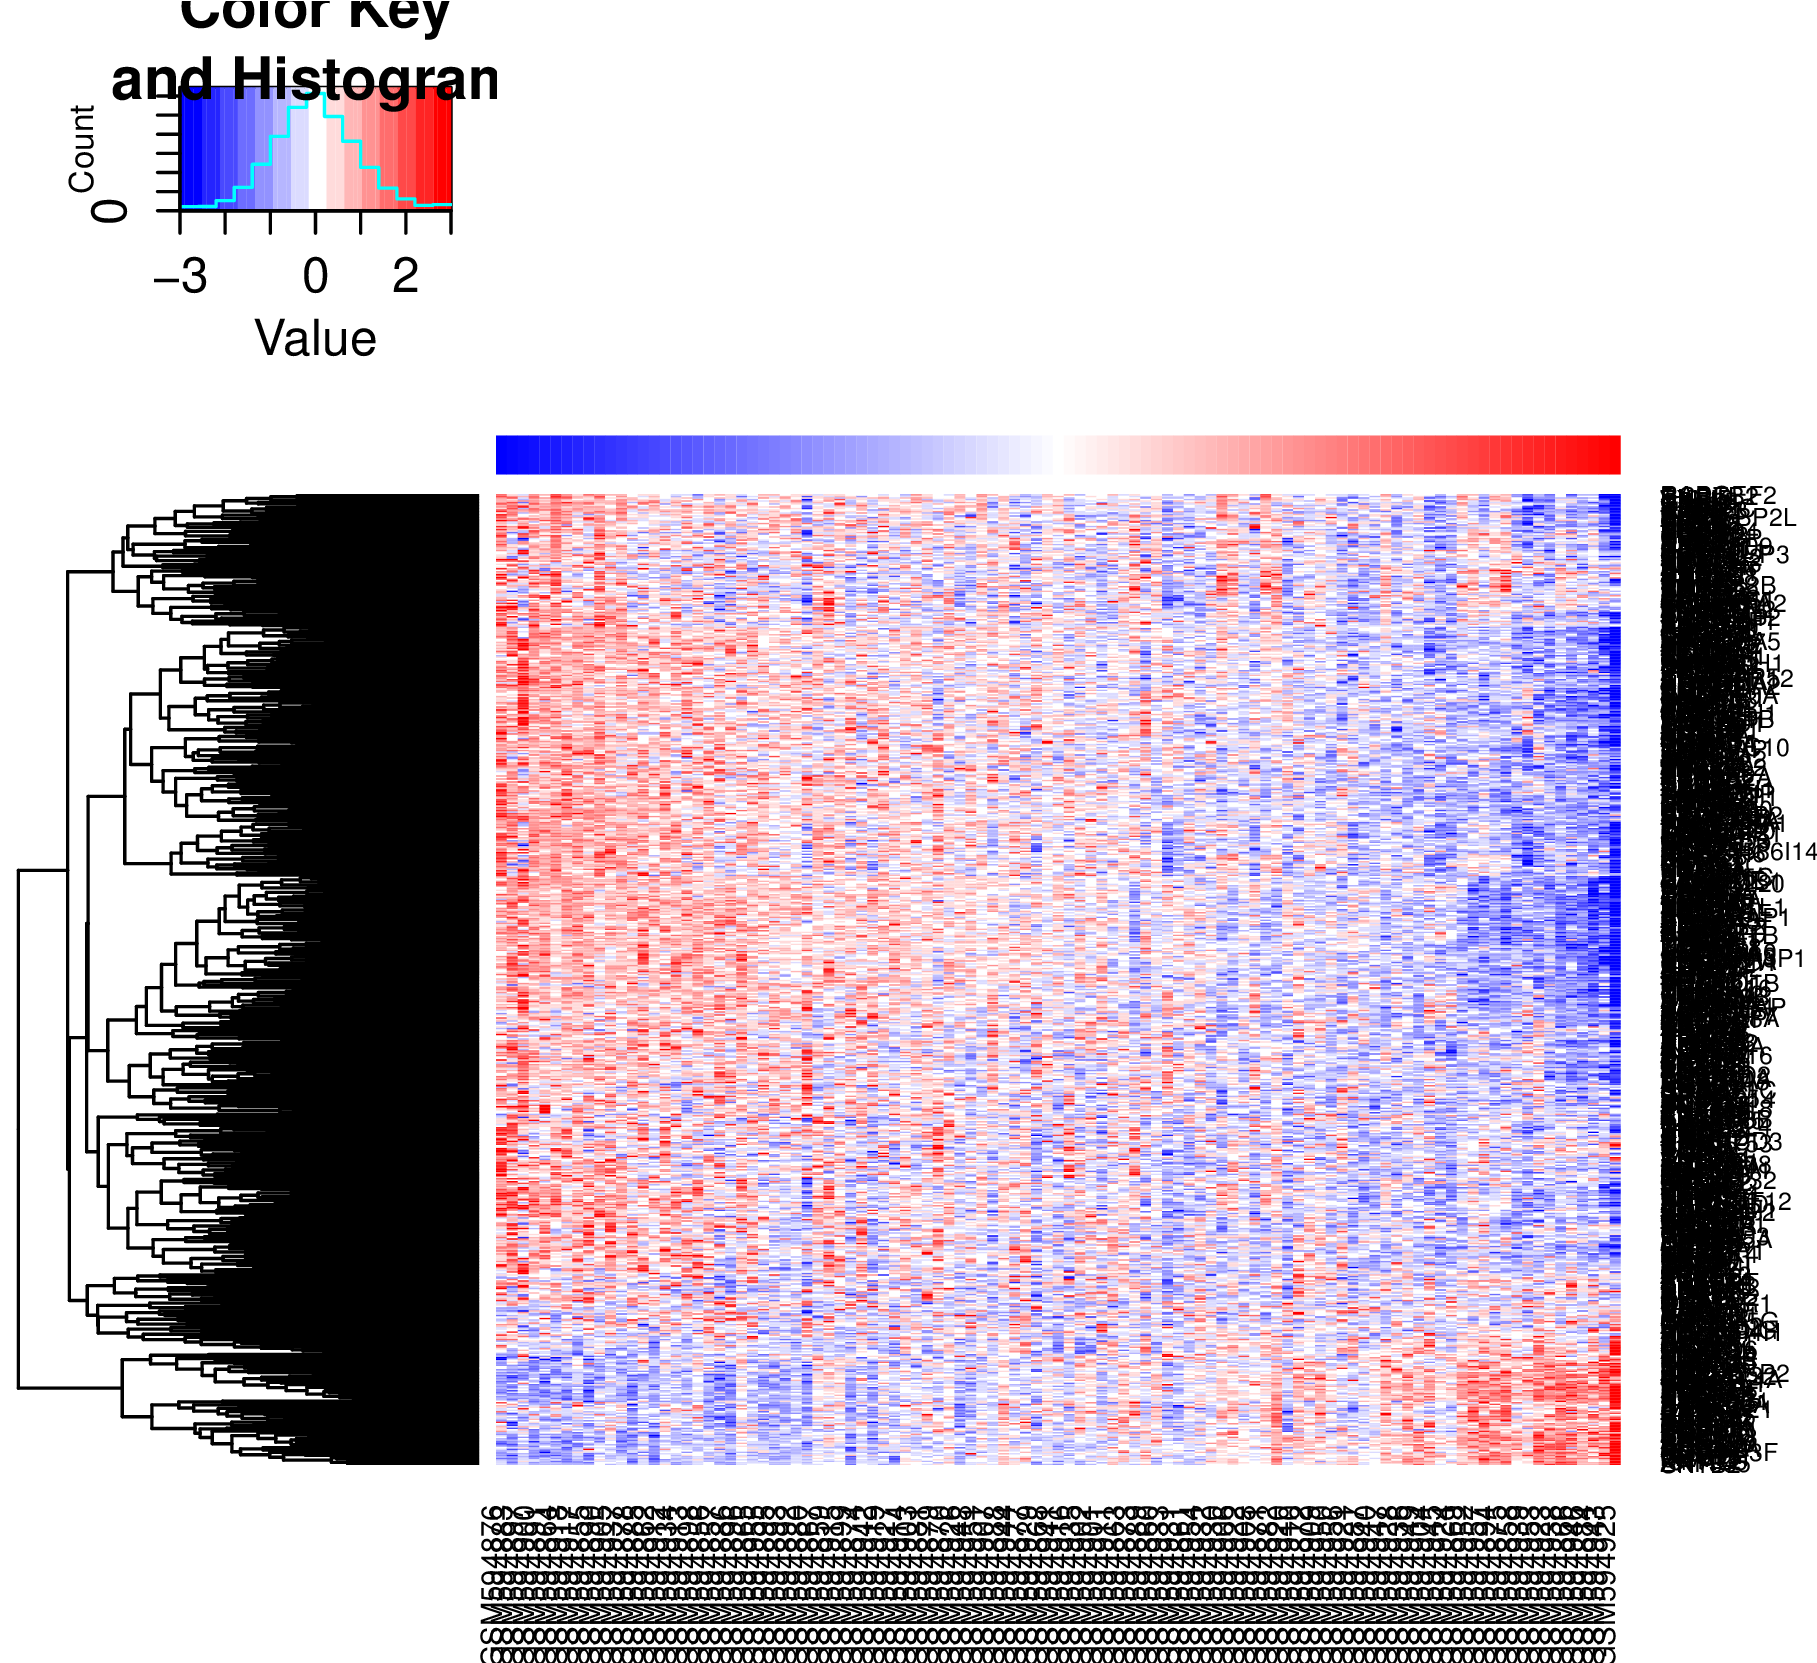
\includegraphics[width=0.45\linewidth]{results1/crmeta_original}
	\caption[FM metagene and Creighton's cancer data]{(insert Creighton heatmaps)}
	\label{fig:fmmetacr1}
\end{figure}

\begin{figure}[htp!]
	\centering
	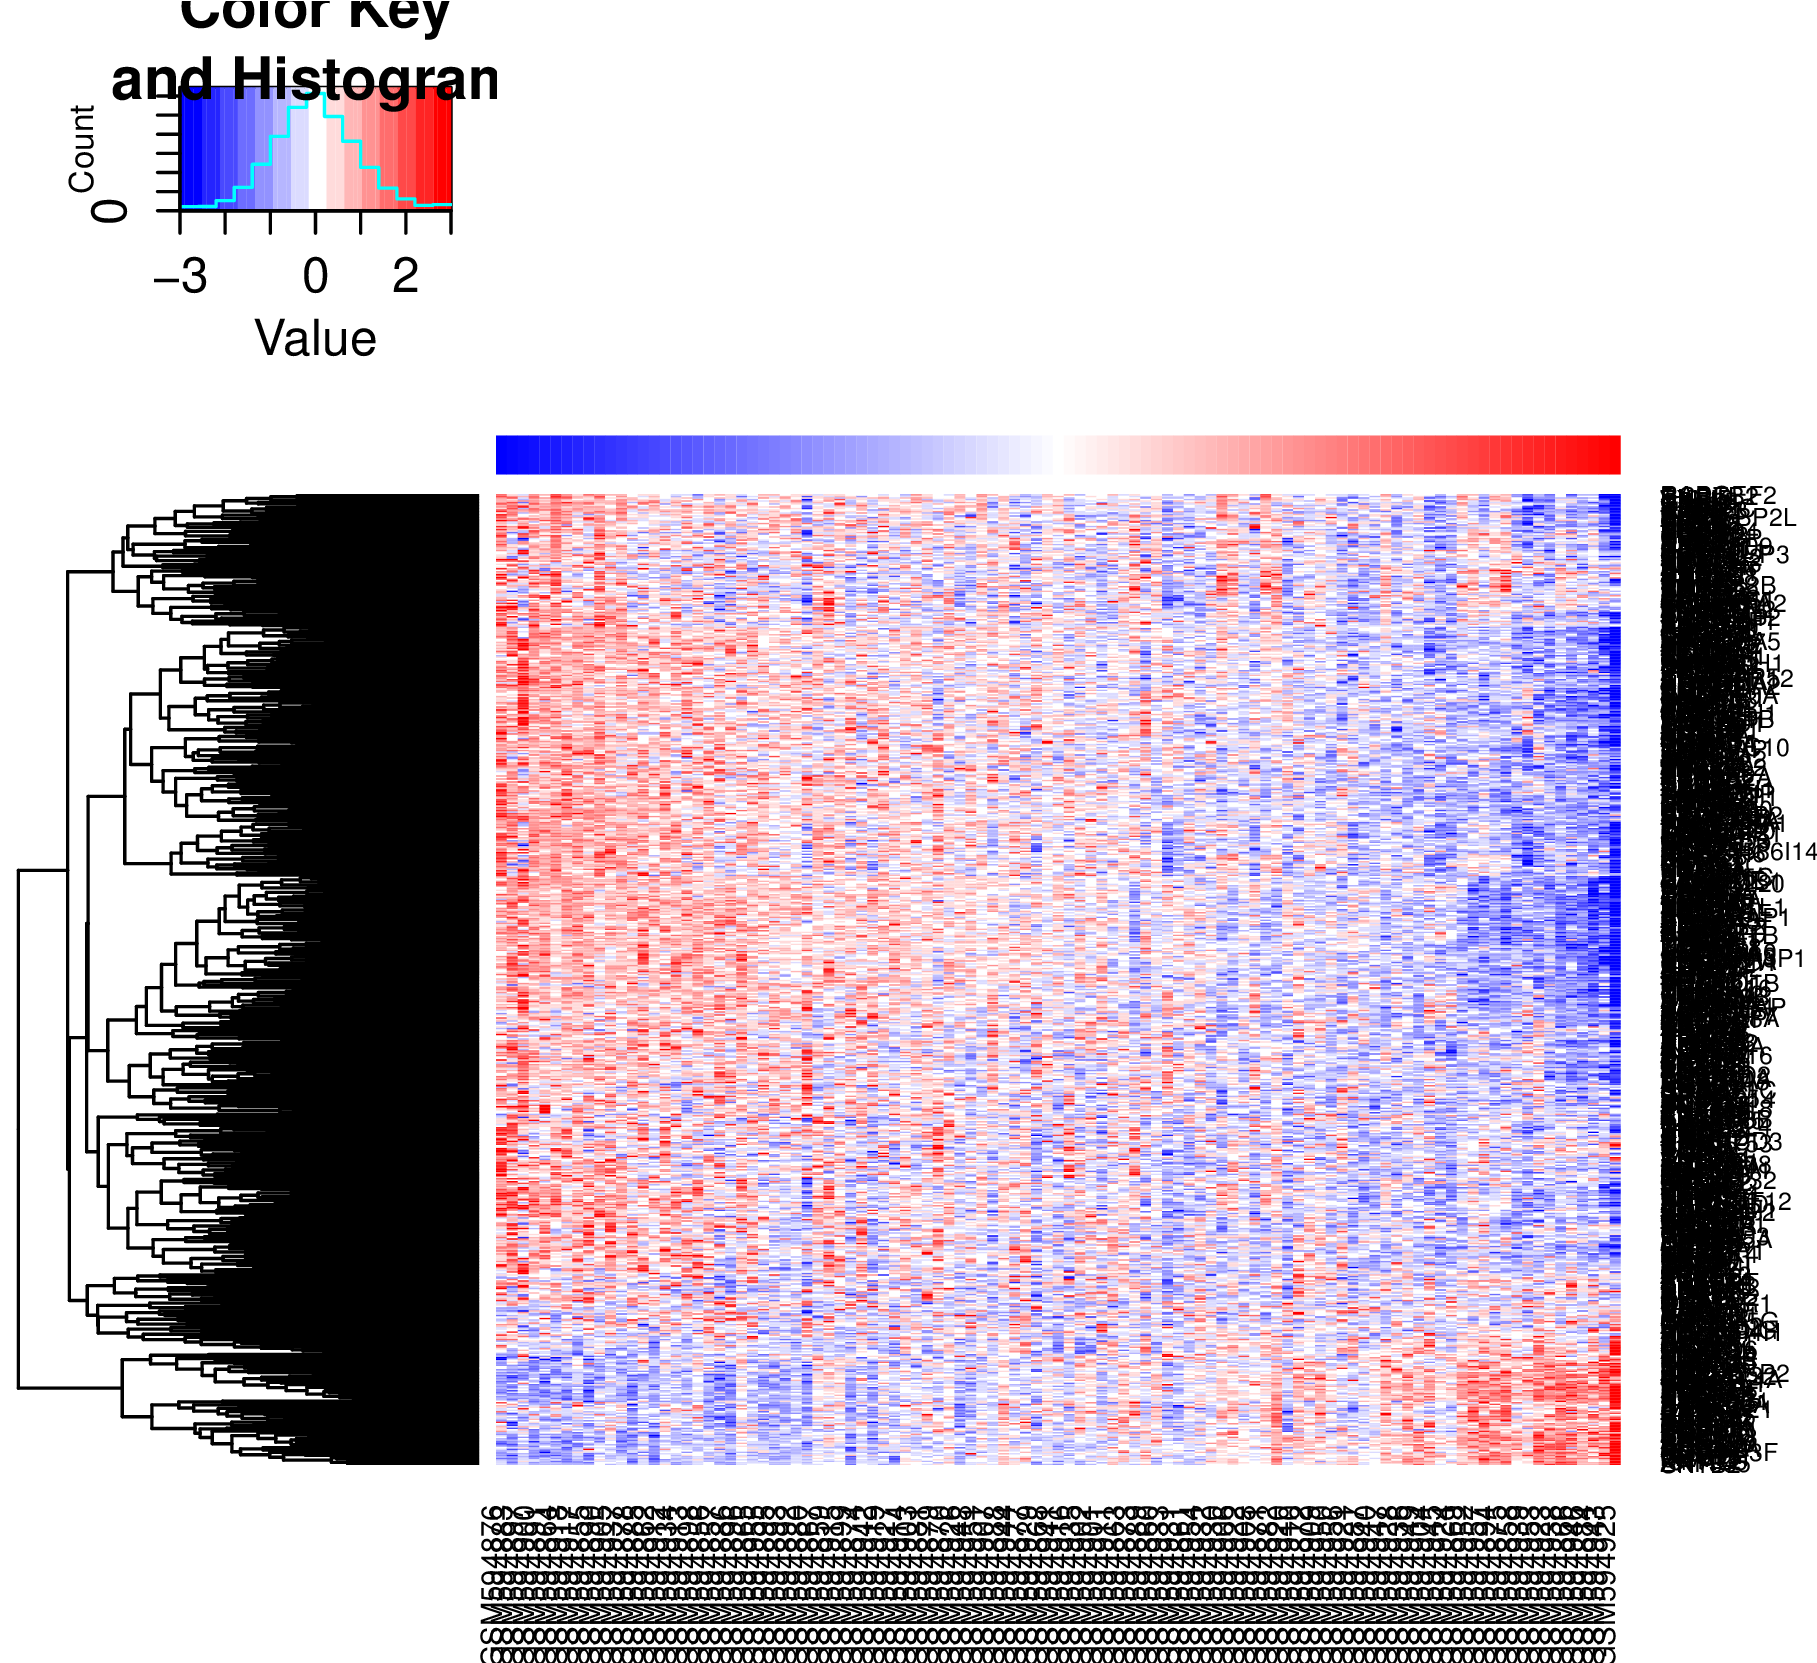
\includegraphics[width=0.45\linewidth]{results1/crmeta_original}
	\hfill
	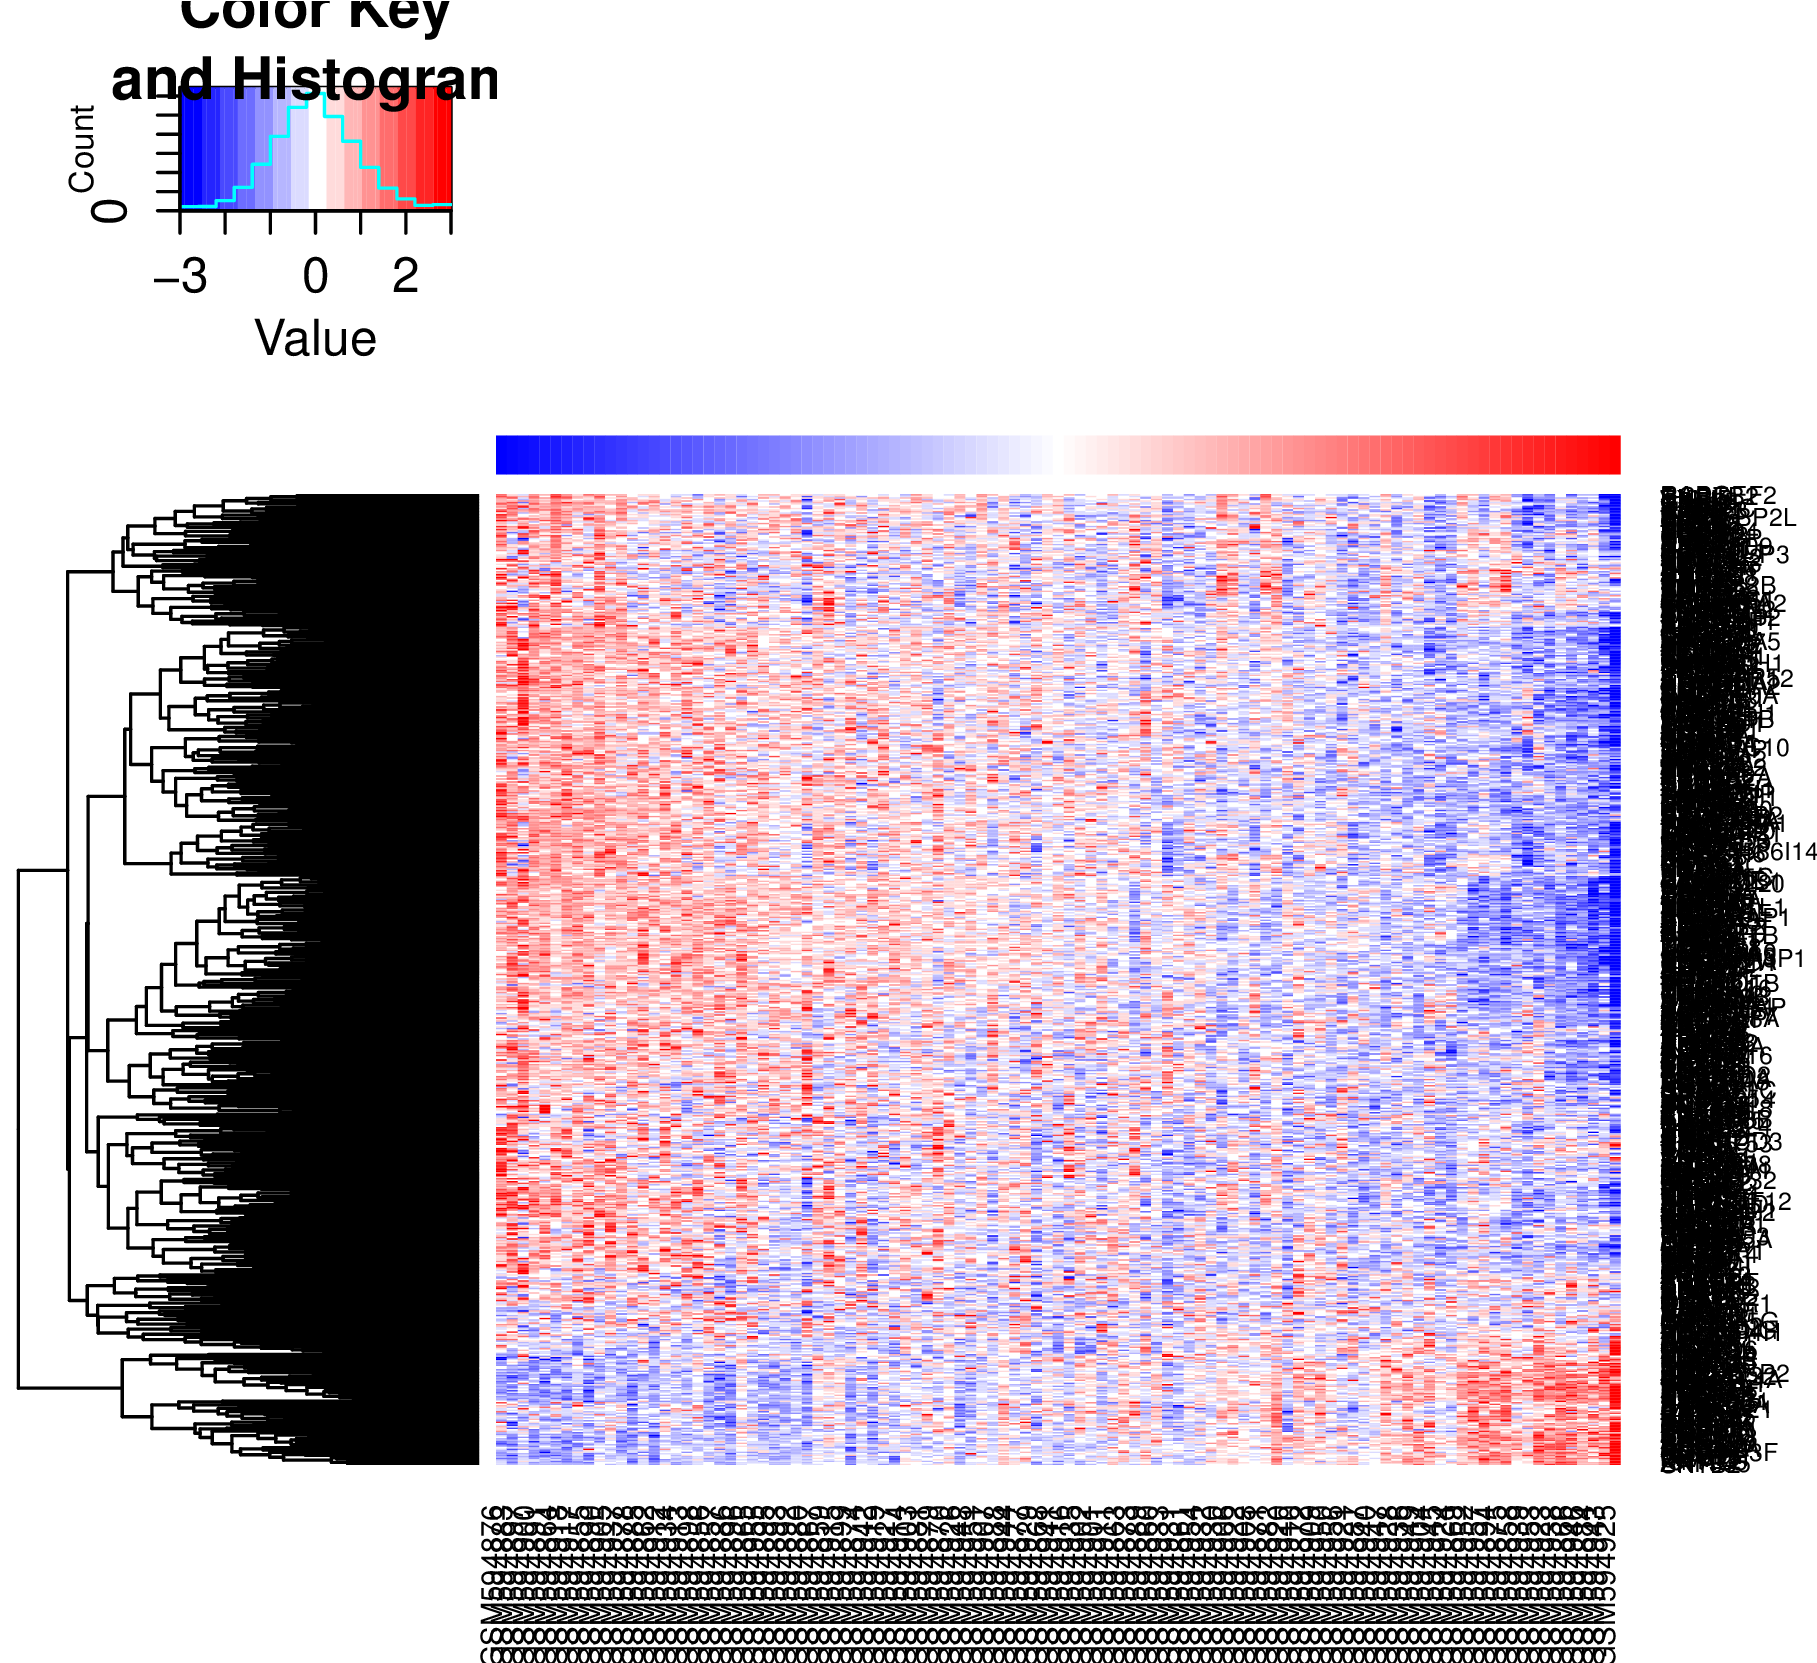
\includegraphics[width=0.45\linewidth]{results1/crmeta_original}
	\caption[FM metagene and sample \gls{bmi}/\gls{bmi} status in Creighton's data]{(insert figure of box plot and scatter plot for Creighton data)}
	\label{fig:fmmetaboxcr1}
\end{figure}

Next, the transformation matrix was applied to the \gls{icgc} cancer data and resulting metagenes were compared with the gene expression and sample \gls{bmi}/\gls{bmi} status.
As evident in \cref{fig:fmmetaicgc1}, FM's obesity metagene scores appeared to reflect the gene expression of FM's obesity associated genetic signature.
However, as with all the results in this section so far, FM's obesity metagene did not significantly associate with any of the \gls{icgc} cancer data (\cref{fig:fmmetaboxicgc1}).

\begin{figure}[htp!]
	\centering
	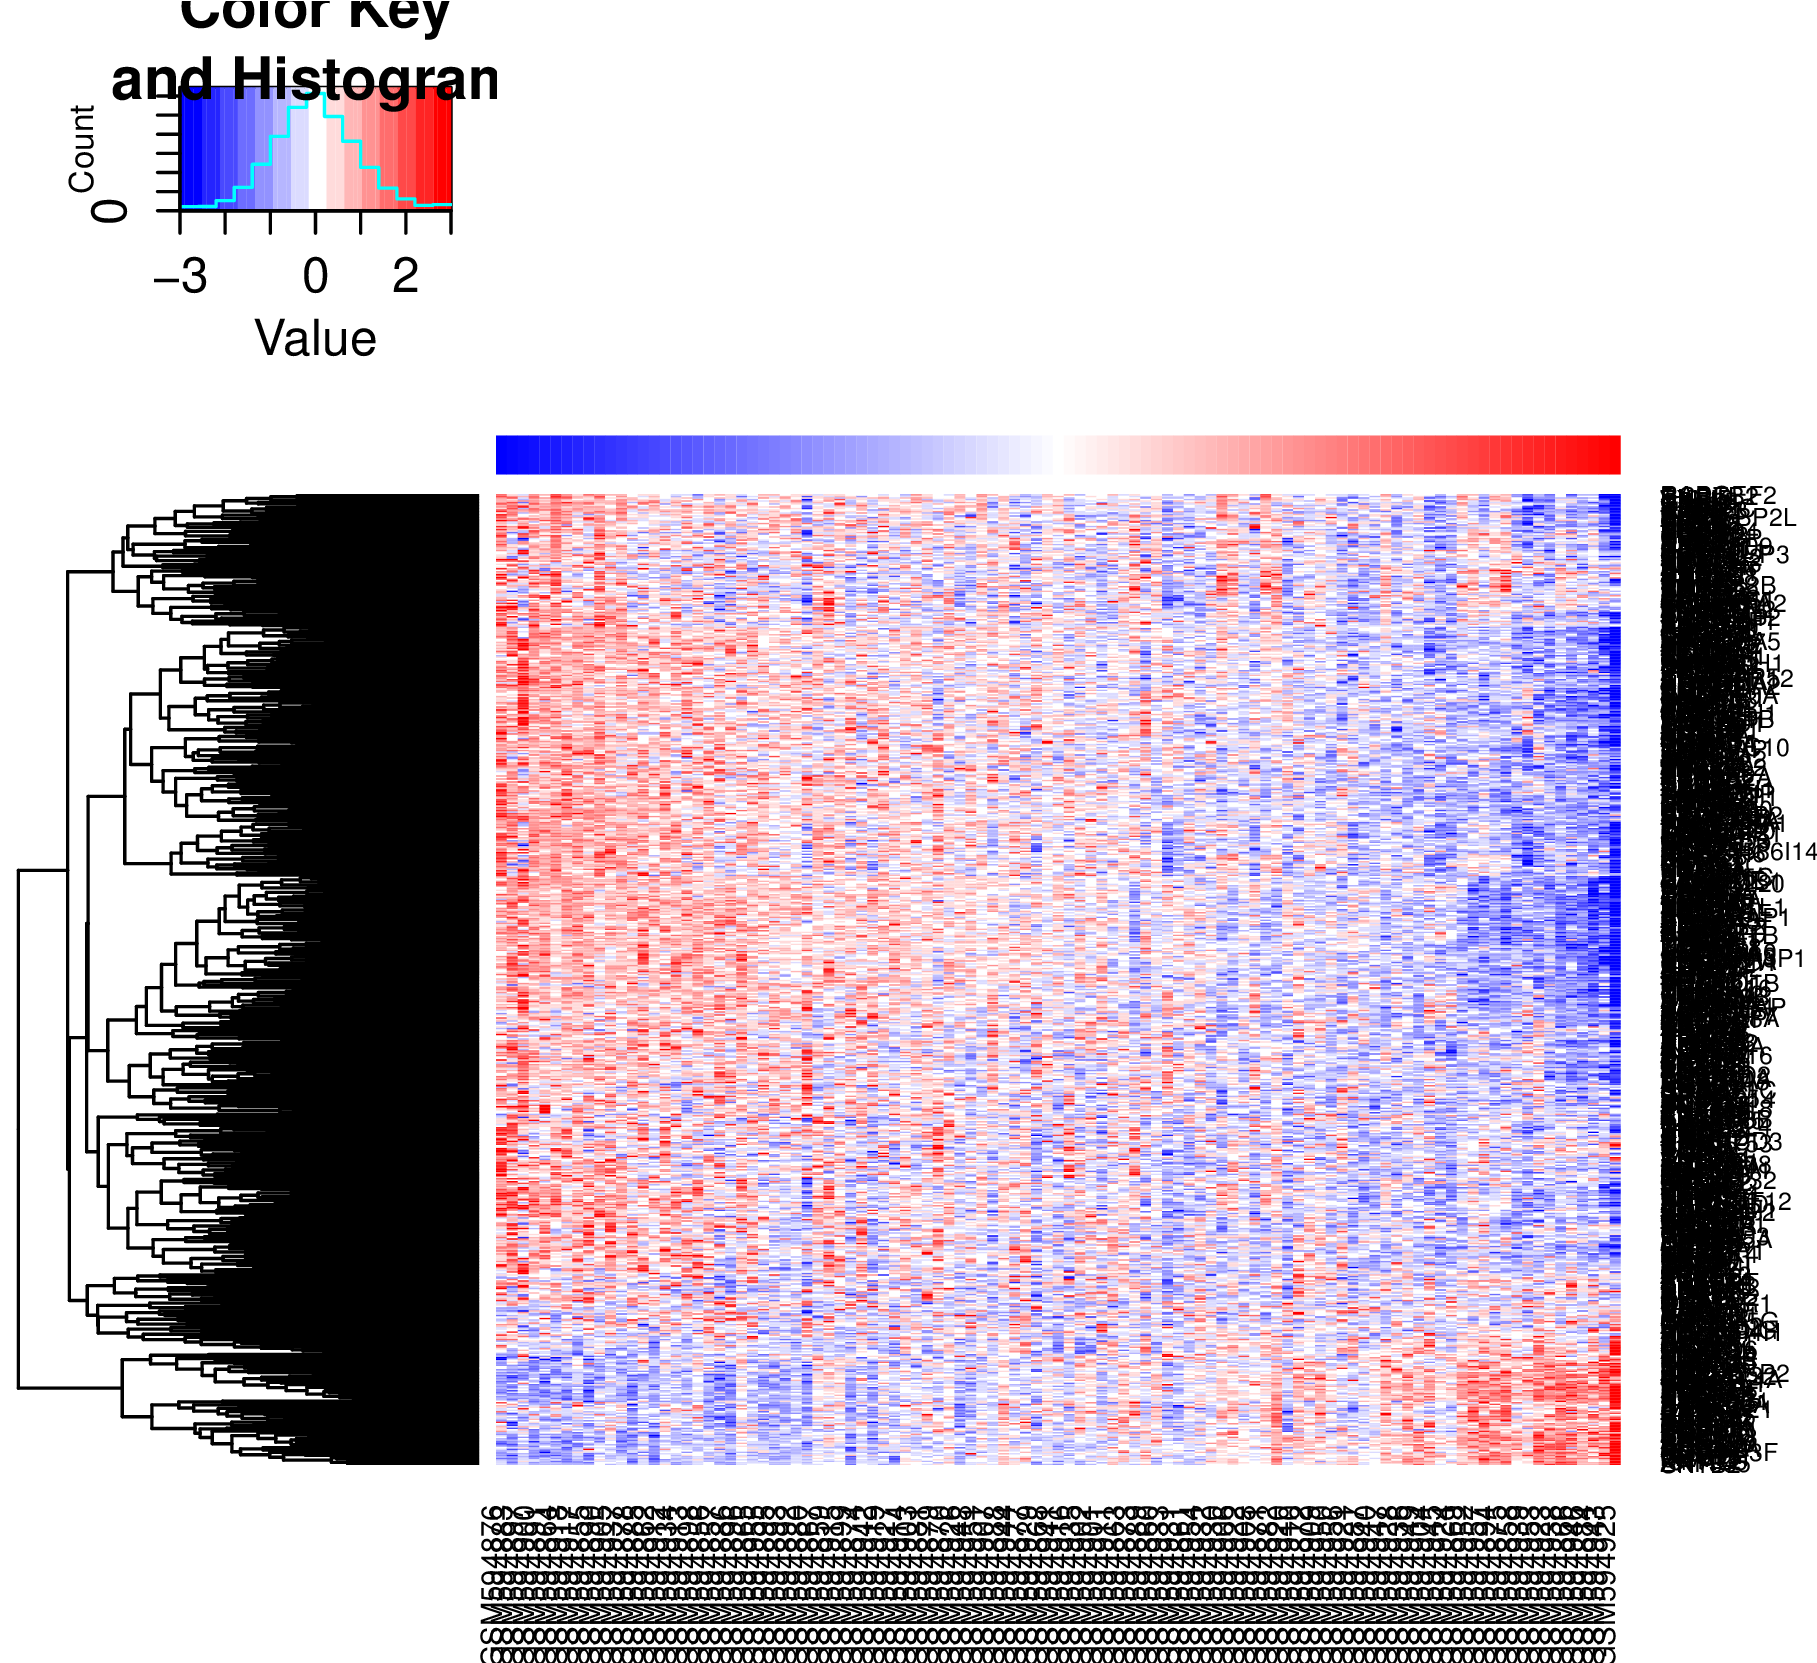
\includegraphics[width=0.45\linewidth]{results1/crmeta_original}
	\hfill
	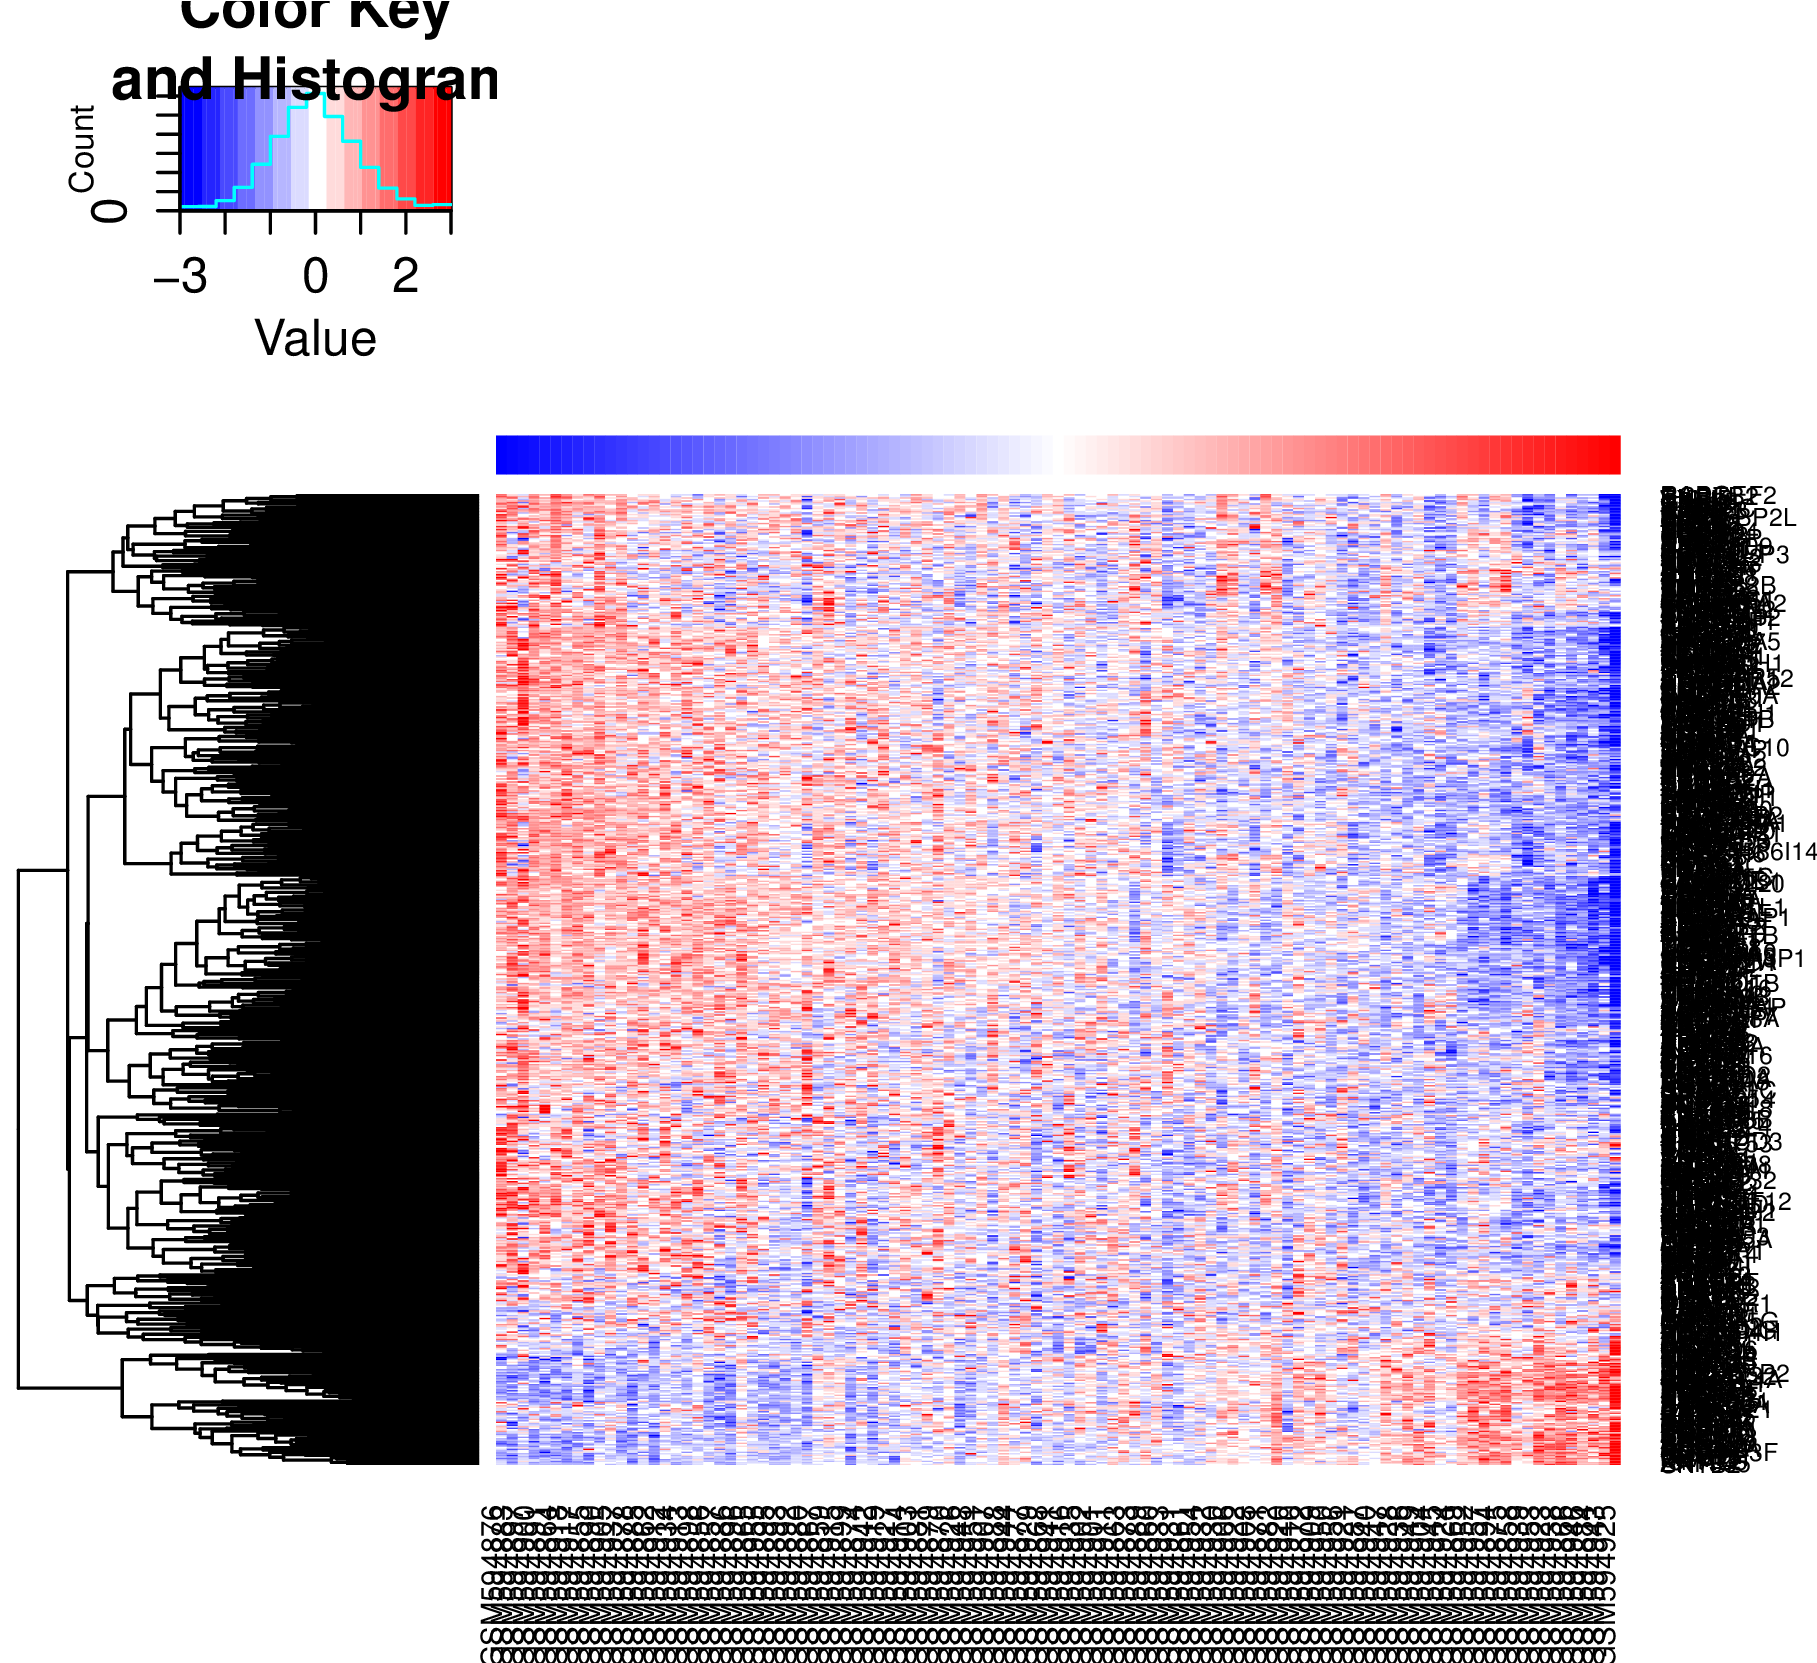
\includegraphics[width=0.45\linewidth]{results1/crmeta_original}
	\caption[FM metagene and \gls{icgc} cancer data]{(insert ICGC heatmaps)}
	\label{fig:fmmetaicgc1}
\end{figure}

\begin{figure}[htp!]
	\centering
	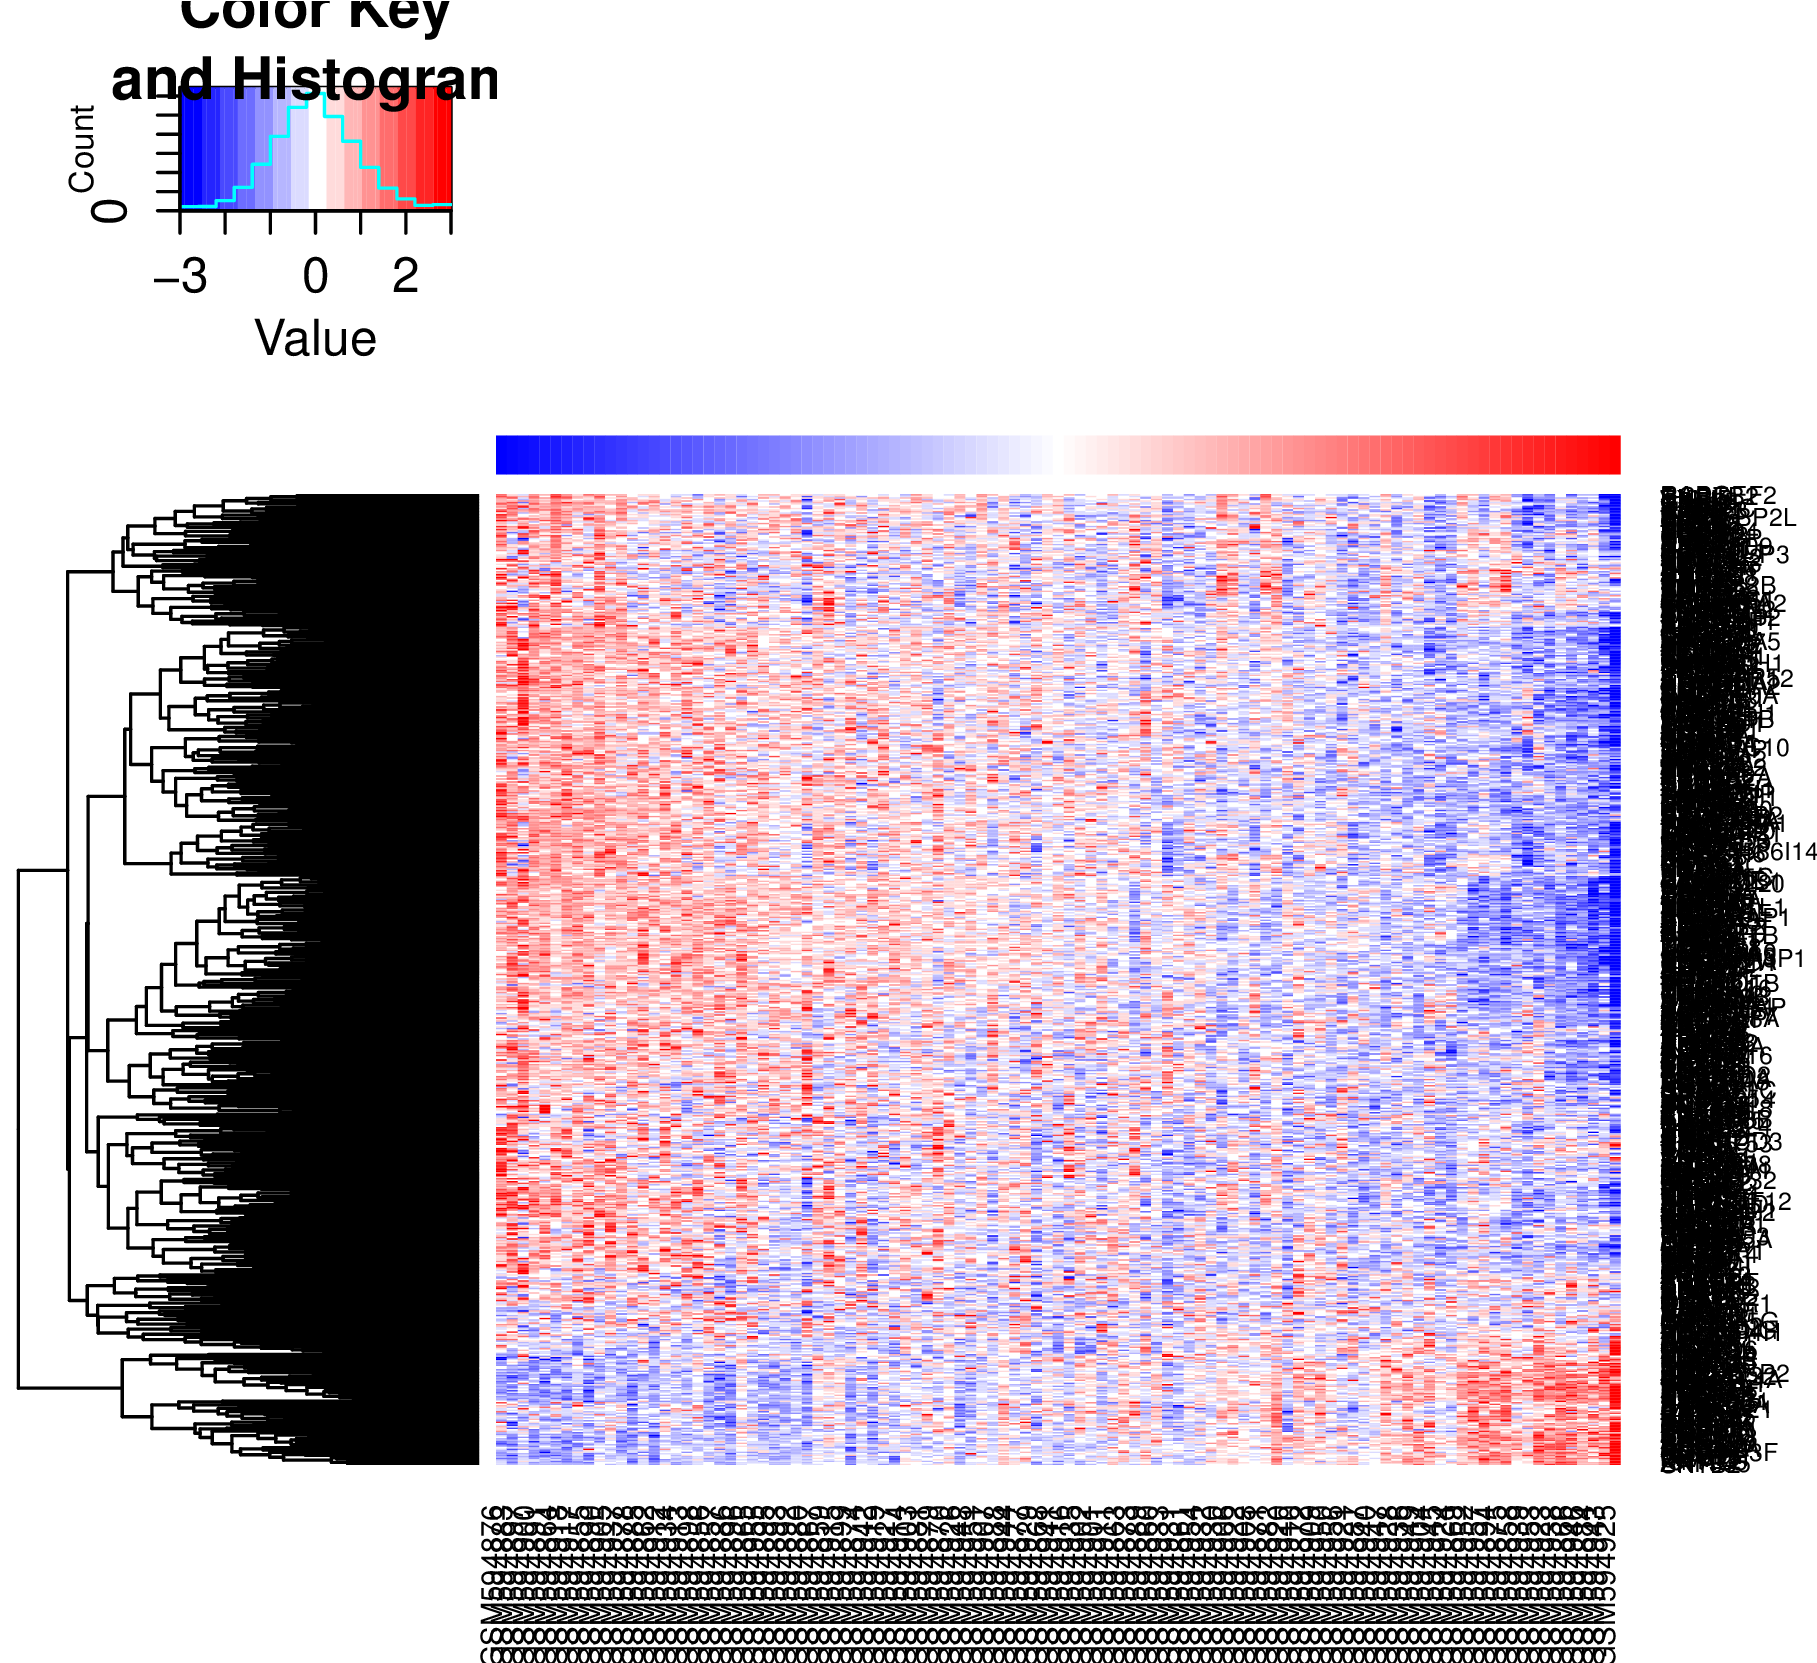
\includegraphics[width=0.45\linewidth]{results1/crmeta_original}
	\hfill
	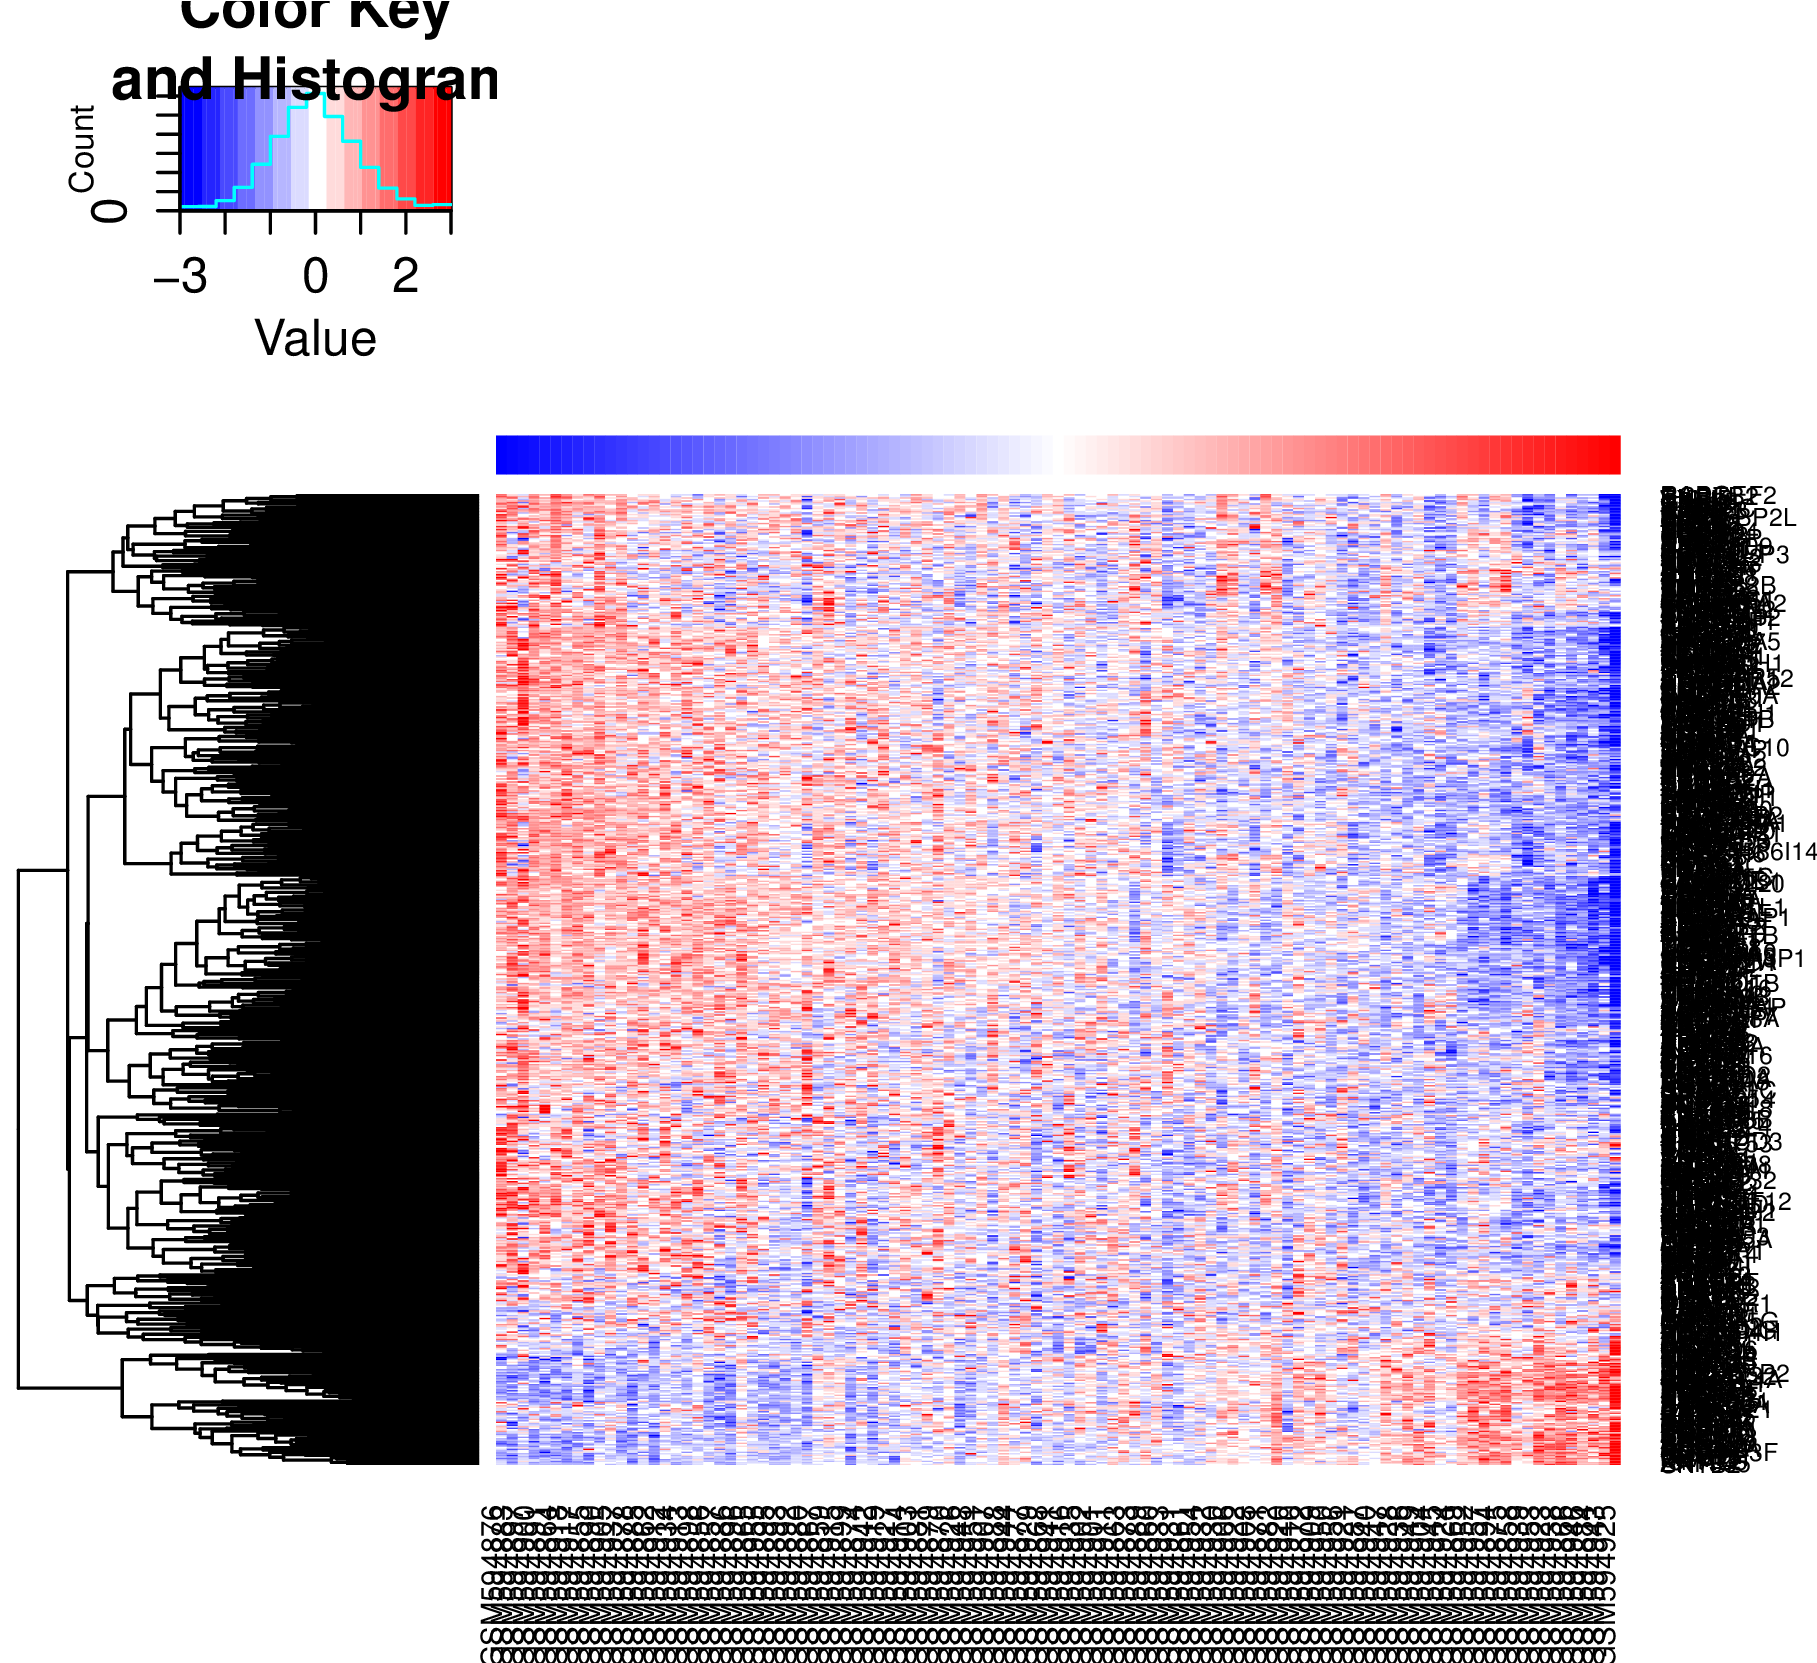
\includegraphics[width=0.45\linewidth]{results1/crmeta_original}
	\caption[FM metagene and sample \gls{bmi}/\gls{bmi} status in \gls{icgc} data]{(insert figure of box plot and scatter plot for Creighton data)}
	\label{fig:fmmetaboxicgc1}
\end{figure}

Lastly, the transformation matrix was applied to Print's data (\cref{fig:fmmetaboxcris1,fig:fmmetacris1}).
Again, FM's obesity metagene scores reflected the gene expression of the samples, did not significantly associate with sample \gls{bmi}/\gls{bmi} status.
\\

\begin{figure}[htp!]
	\centering
	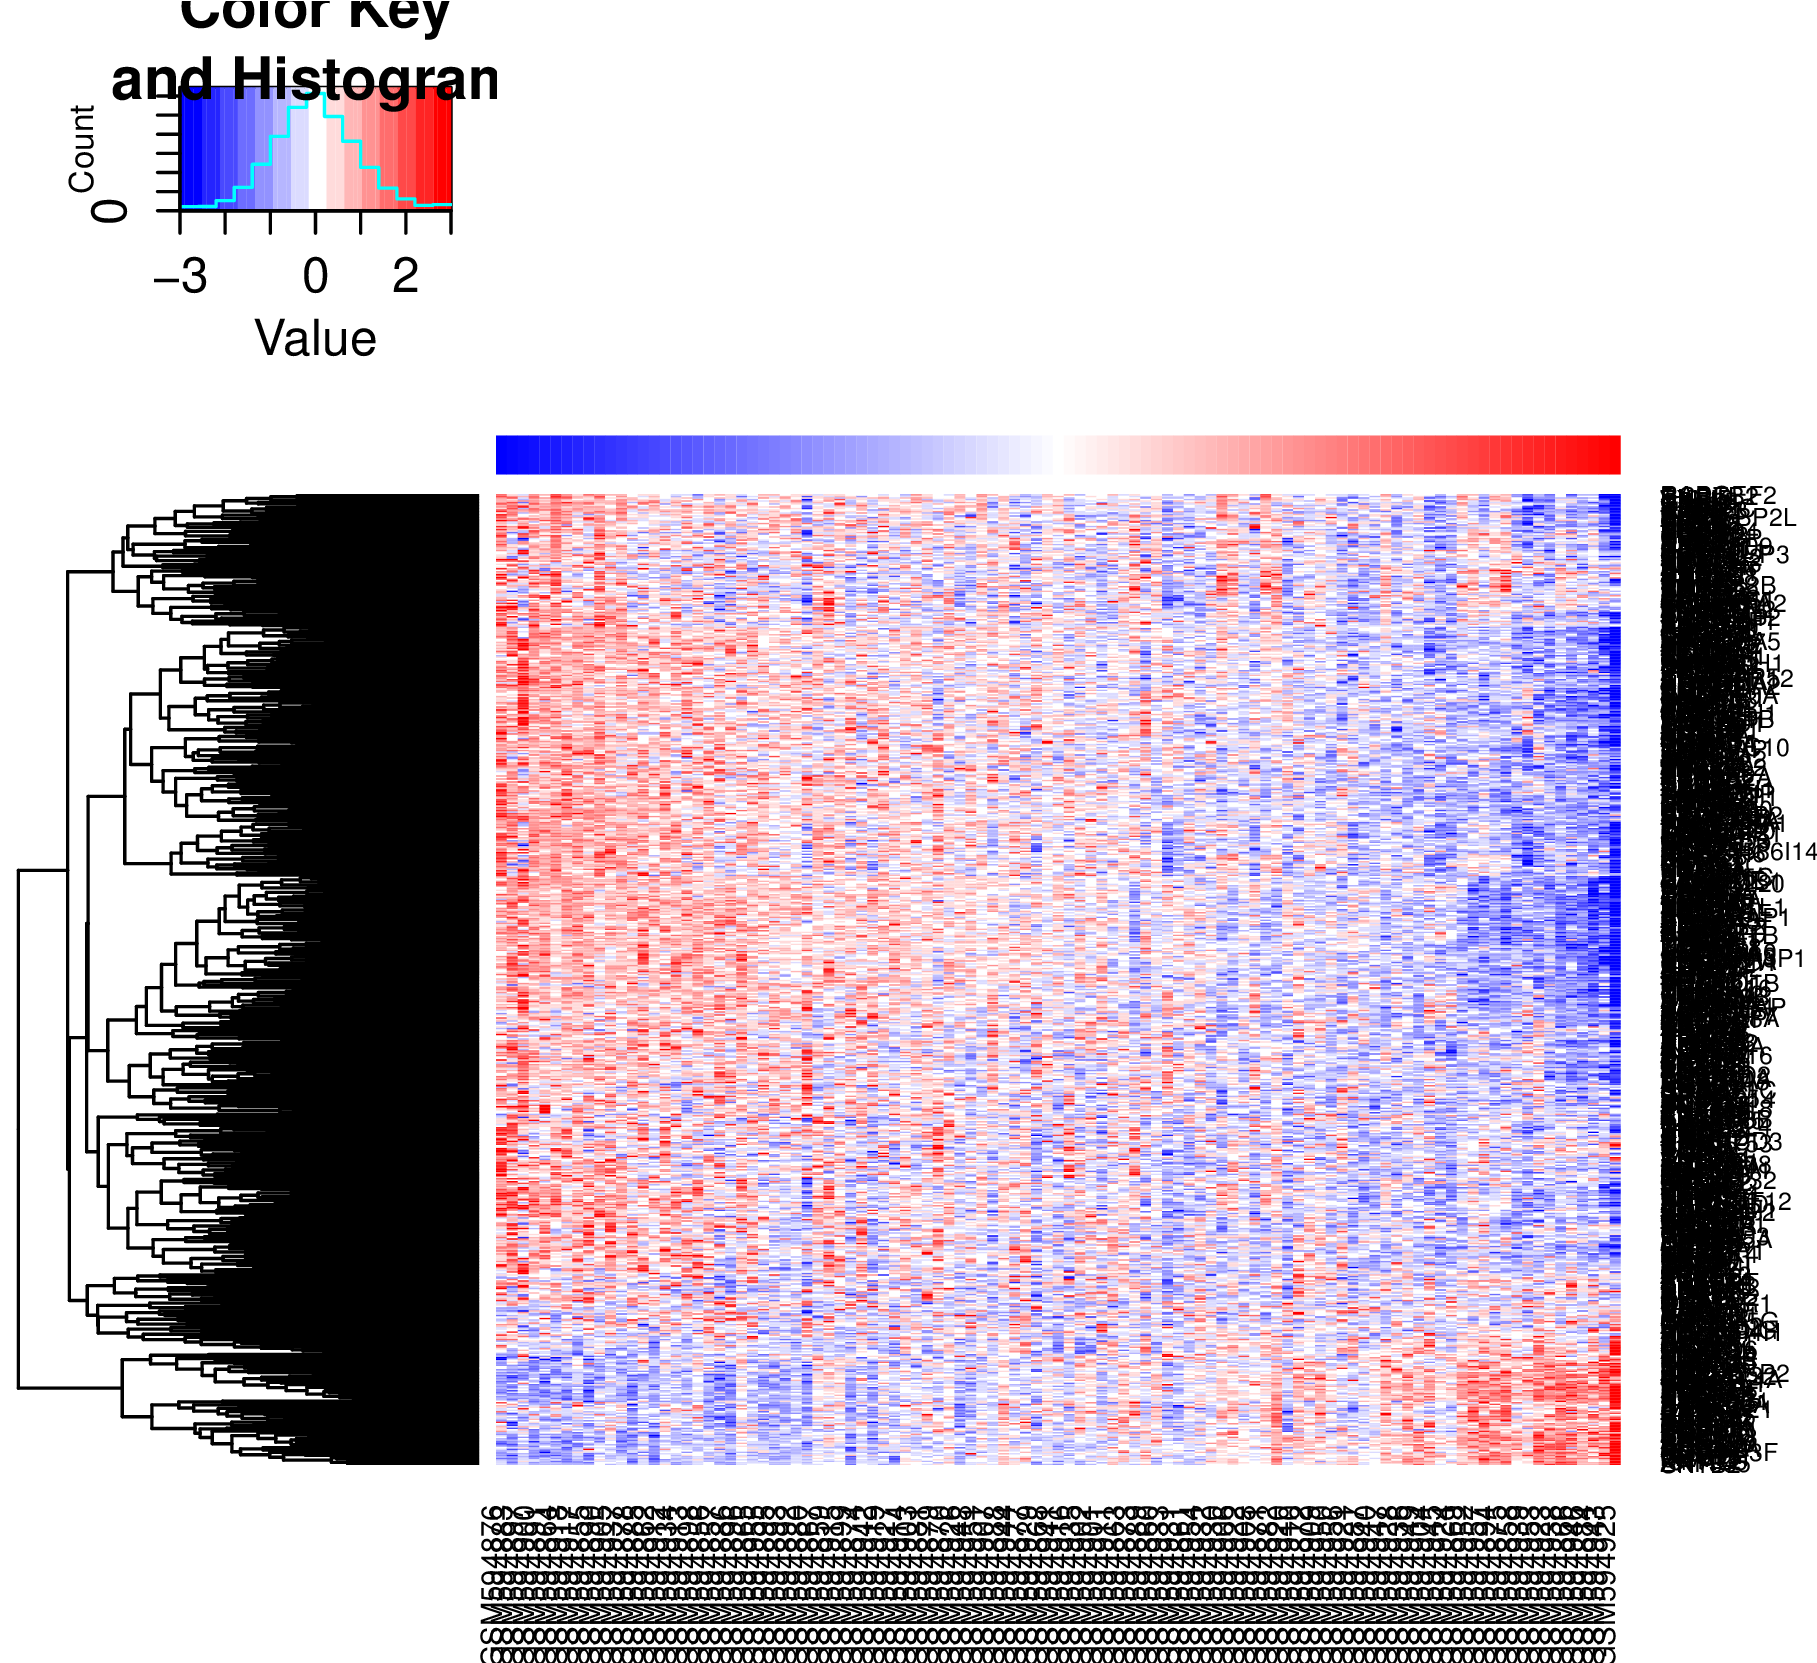
\includegraphics[width=0.45\linewidth]{results1/crmeta_original}
	\hfill
	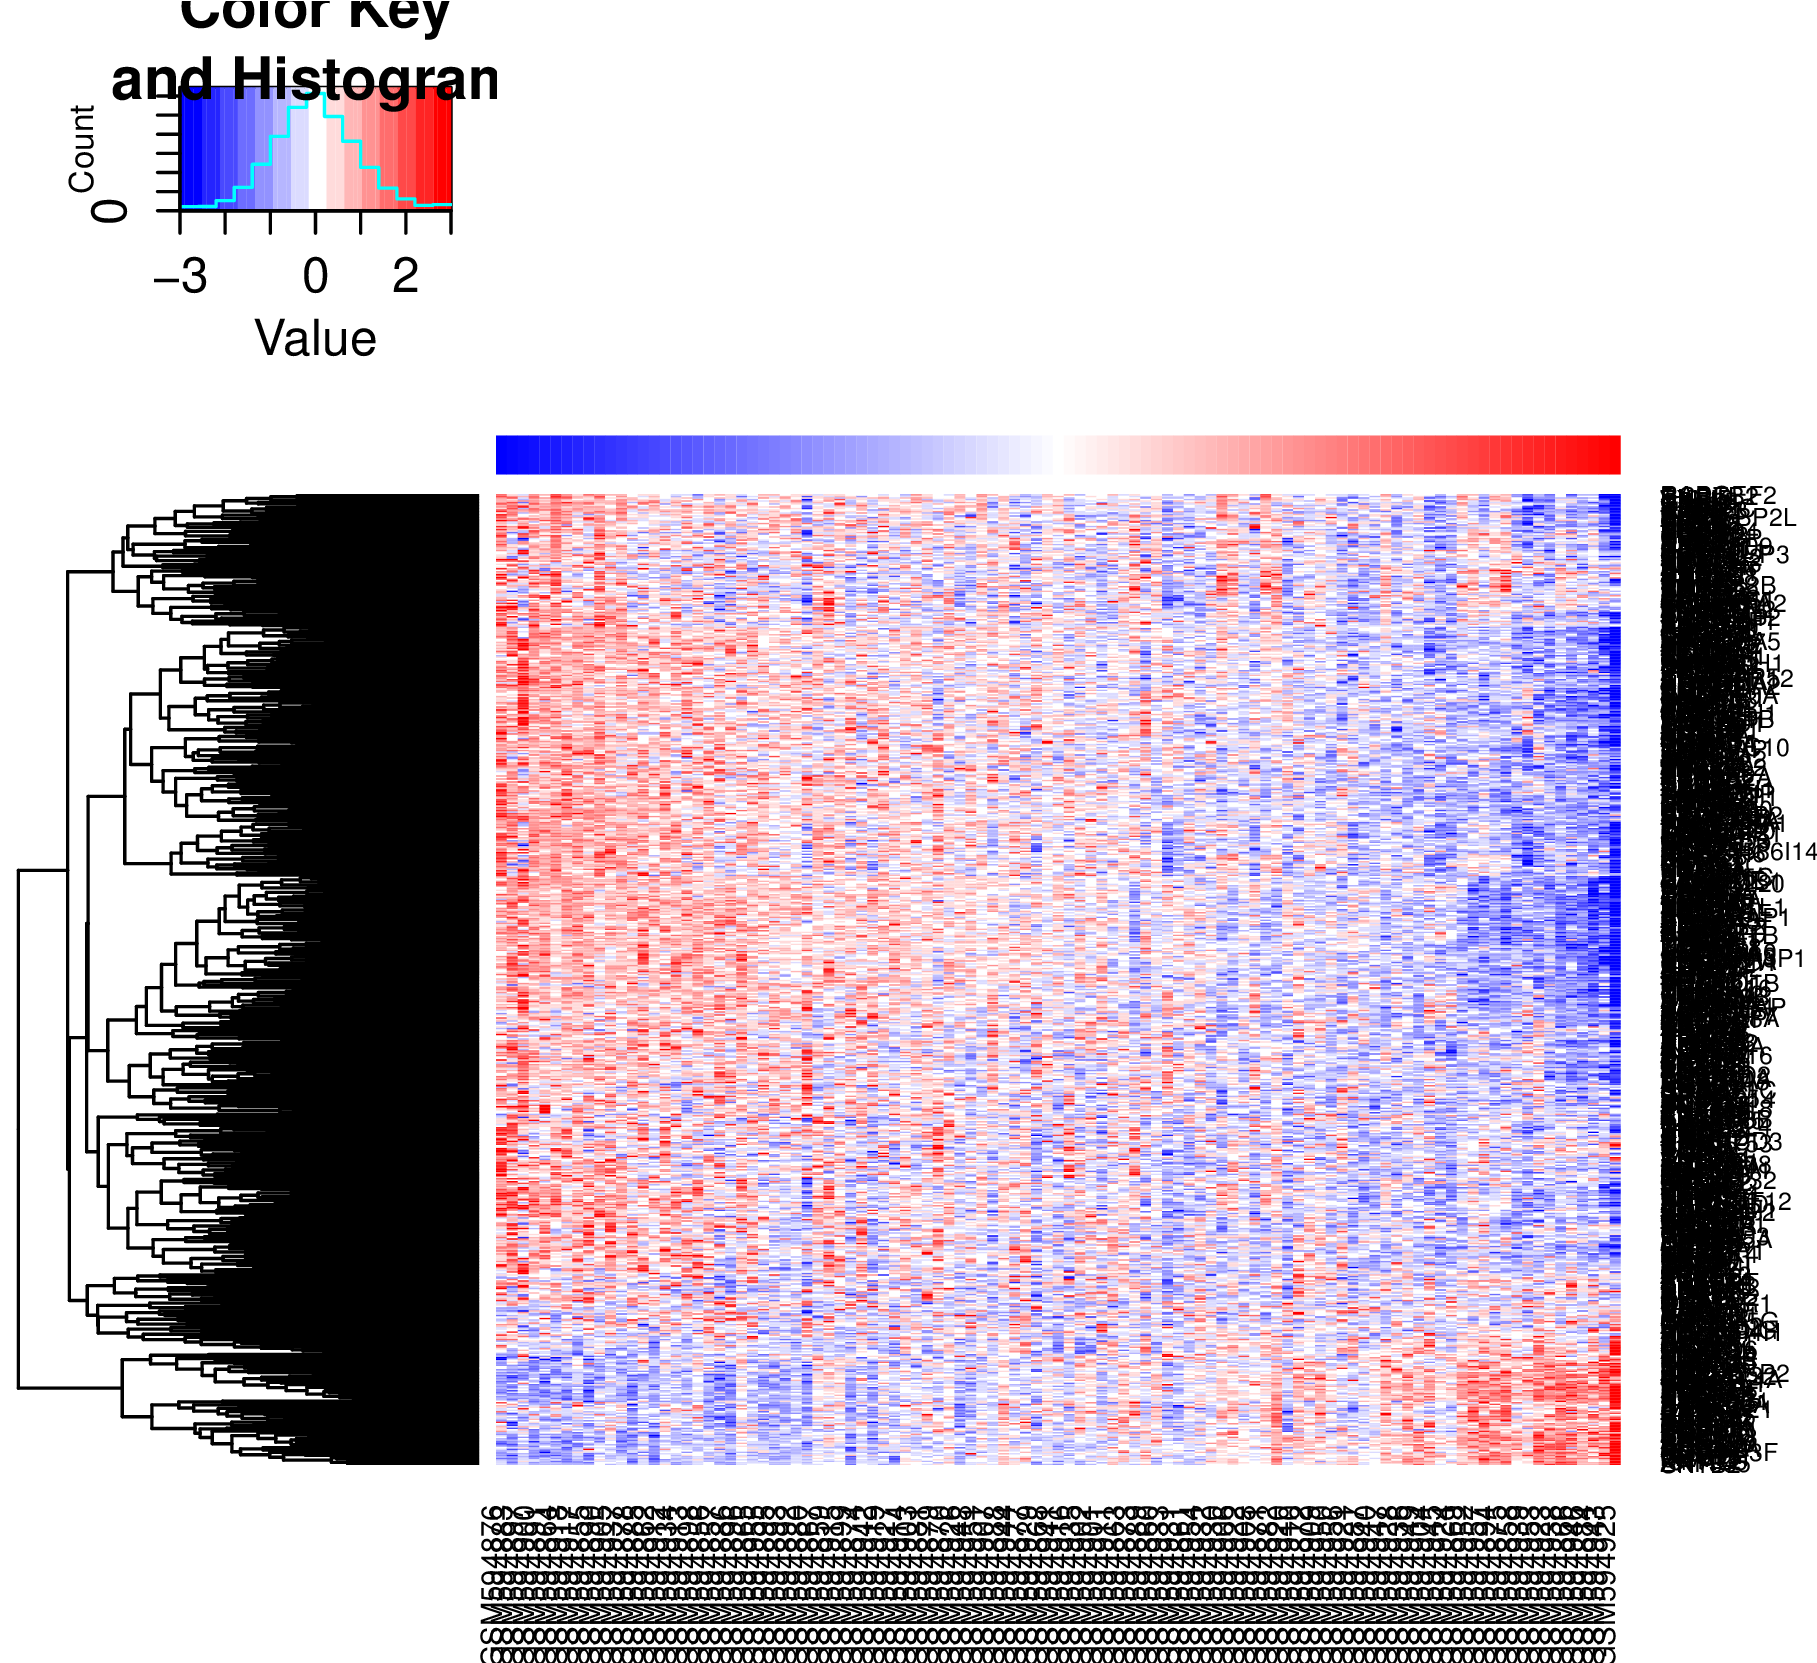
\includegraphics[width=0.45\linewidth]{results1/crmeta_original}
	\caption[FM metagene and Print's cancer data]{(insert Print heatmaps)}
	\label{fig:fmmetacris1}
\end{figure}

\begin{figure}[htp!]
	\centering
	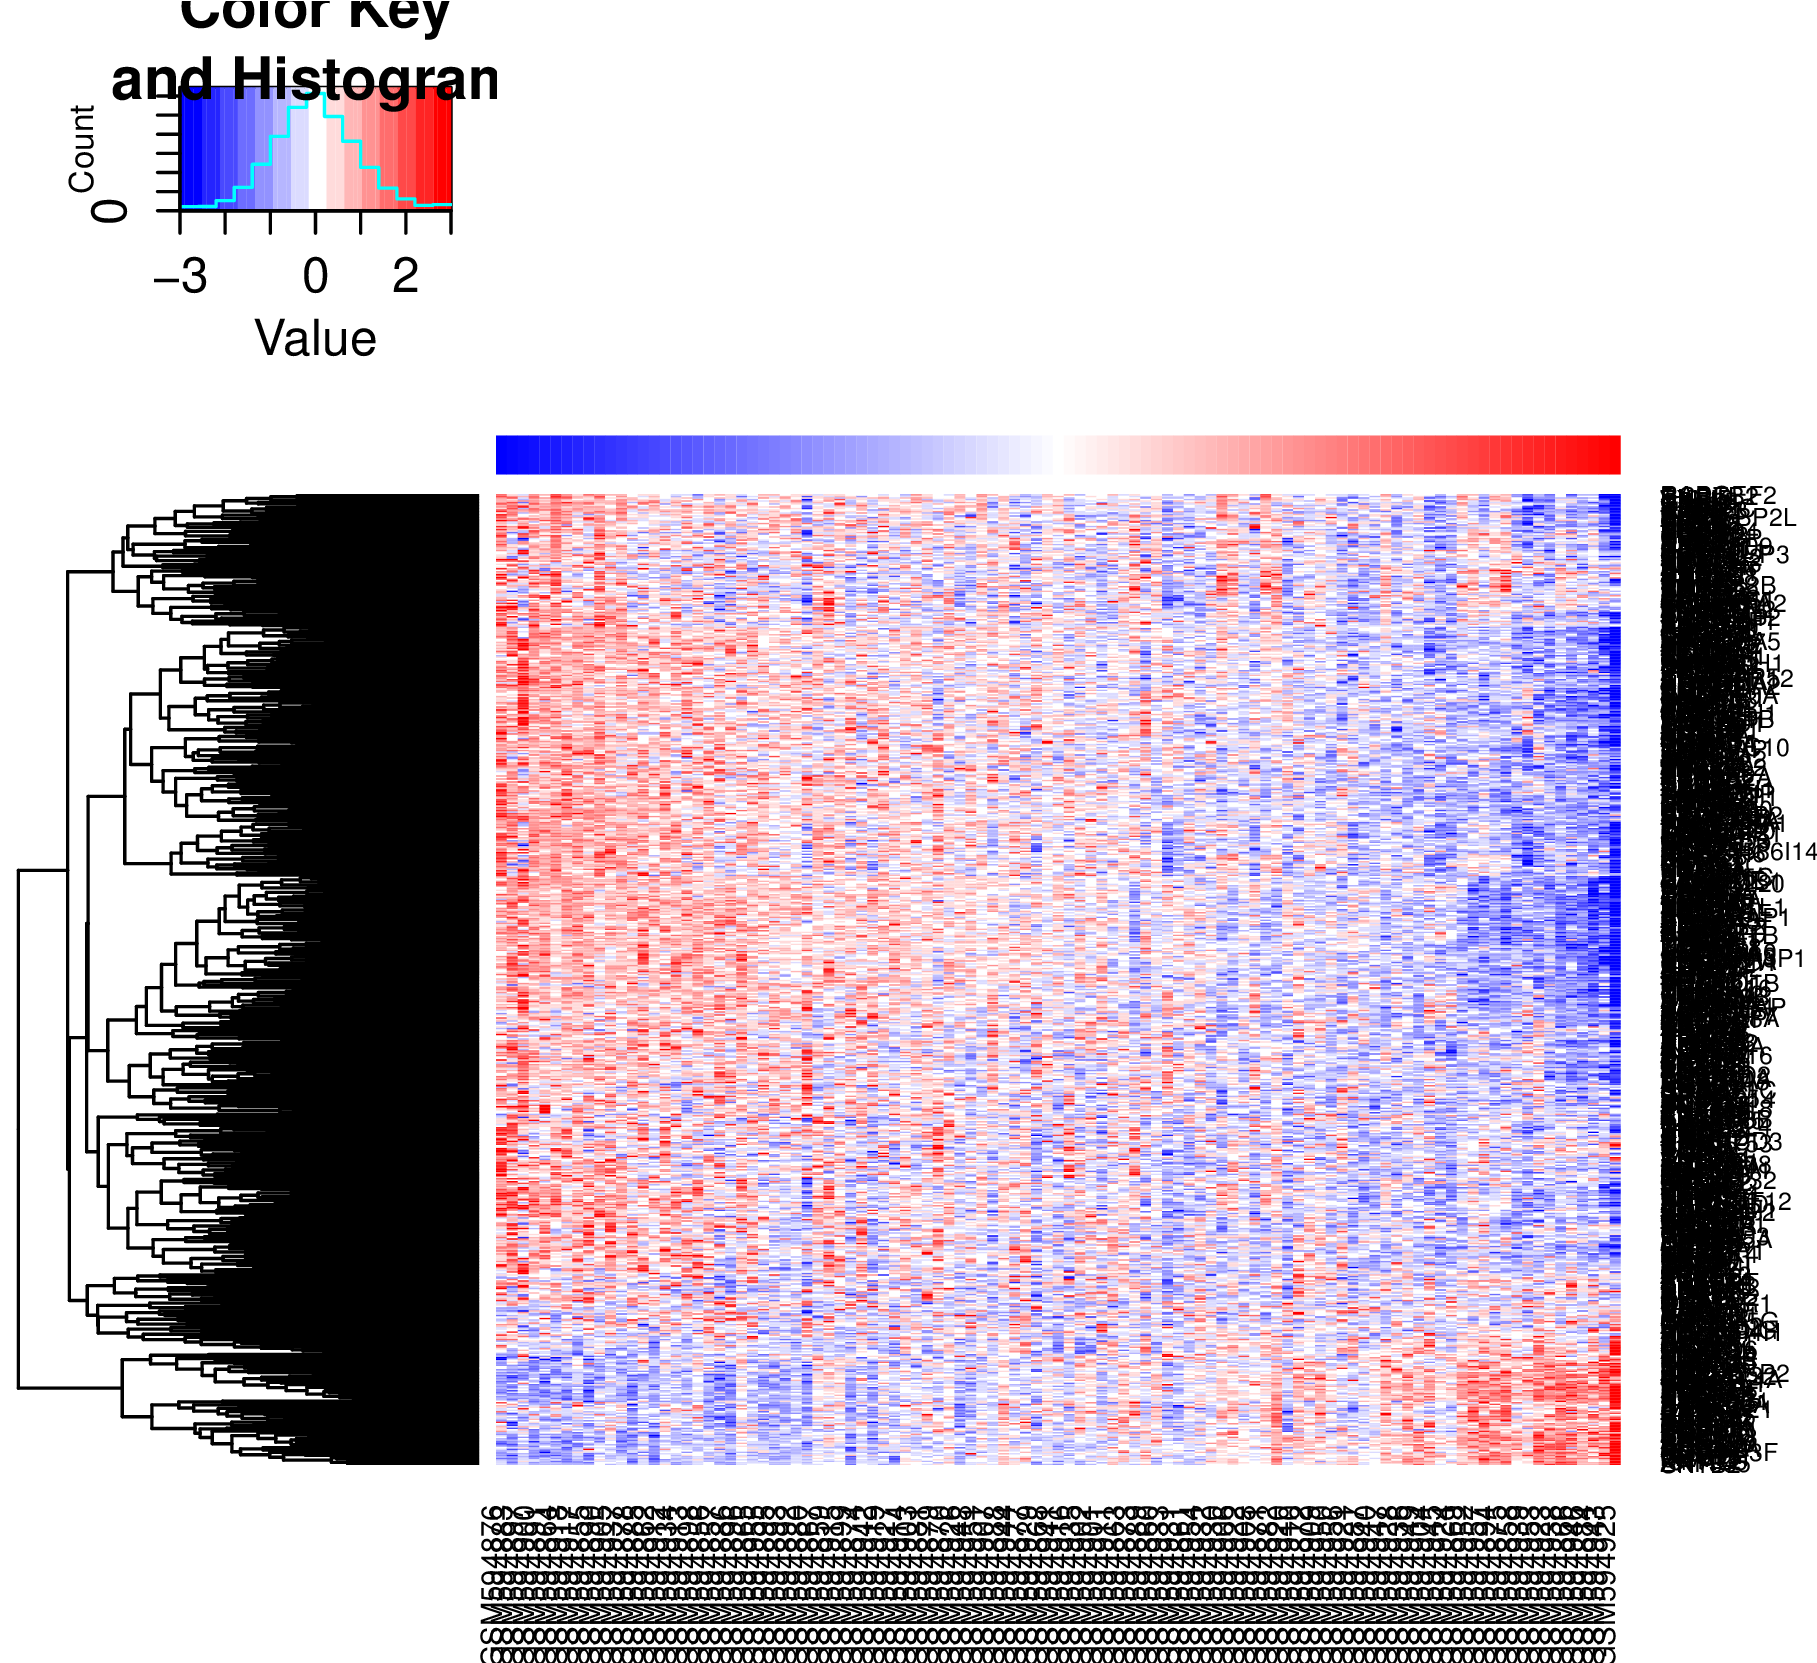
\includegraphics[width=0.45\linewidth]{results1/crmeta_original}
	\hfill
	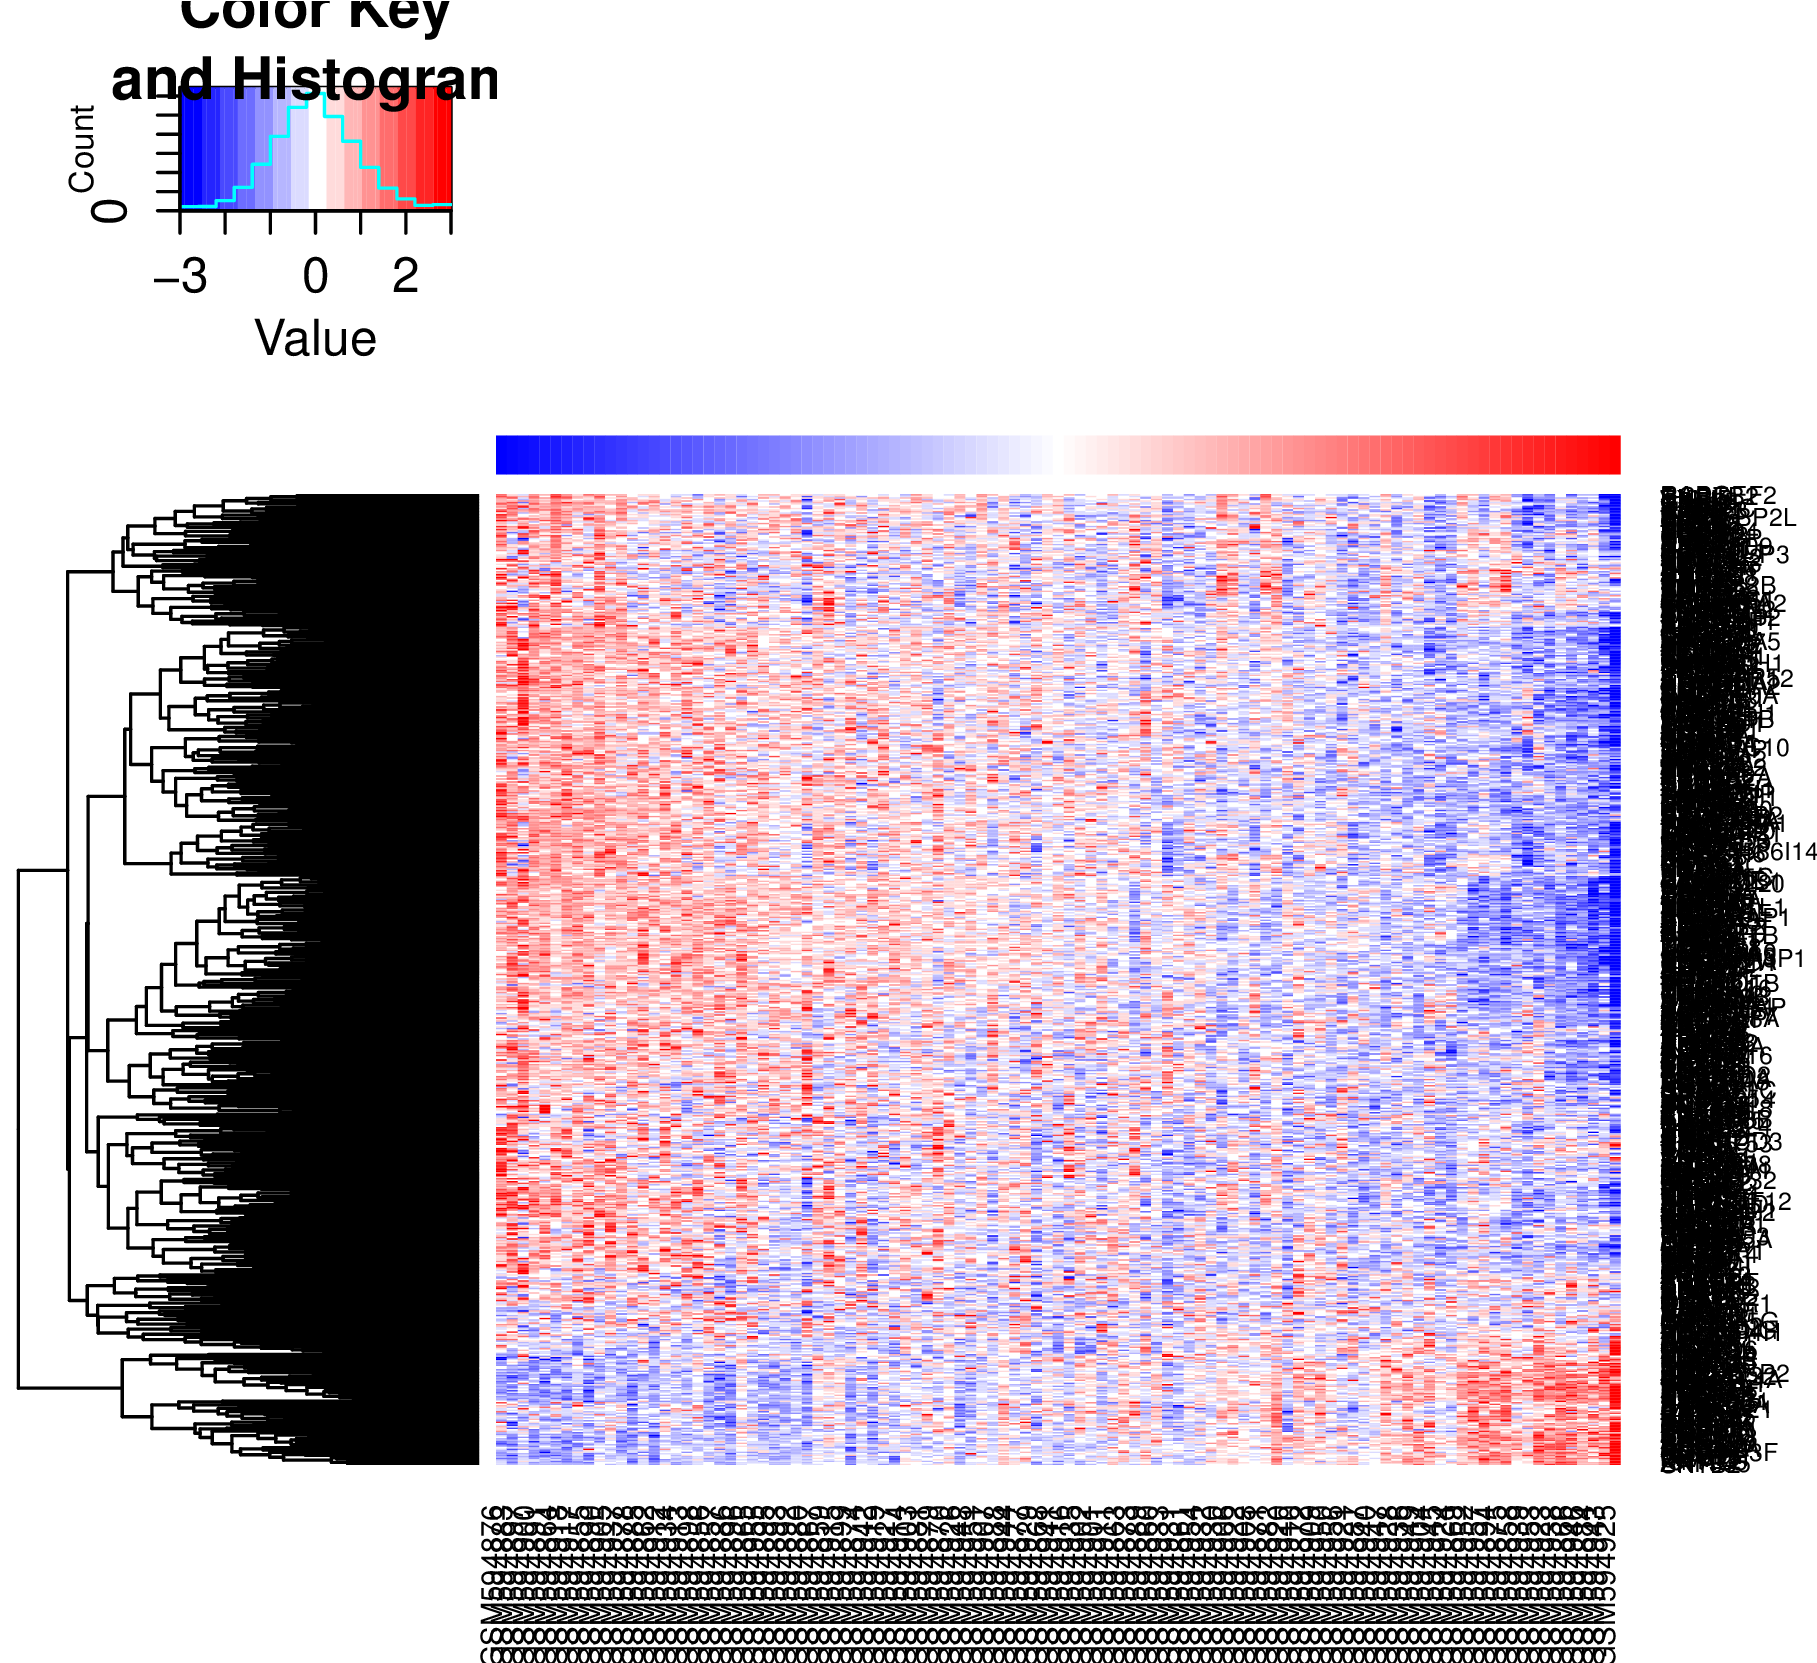
\includegraphics[width=0.45\linewidth]{results1/crmeta_original}
	\caption[FM metagene and sample \gls{bmi}/\gls{bmi} status in Print's data]{(insert figure of box plot and scatter plot for Print's data)}
	\label{fig:fmmetaboxcris1}
\end{figure}

\noindent
These results showed that FM's obesity associated metagene was not transferable to other cancer data sets, similar to Creighton's obesity associated metagene.
This meant that neither Creighton's nor FM's obesity associate metagenes may be too specific to the orignial data set in which the signature was identified in.
Furthermore, it may be possible that these obesity associated metagenes may not be related to obesity, but another clinical variable which may be closely related to \gls{bmi}.

\section{New obesity associated genetic signature in \citet{Creighton2012} data set}
\label{sec:creighton_obesity_metagene_new}

Both metagenes generated from Creighton's data and FM's data were able to capture the overall pattern of gene expression of the samples, but did not associate with sample \gls{bmi}/\gls{bmi} status.
One possible reason for this result could be that the obesity associated genetic signatures from Creighton's and FM's study may not have been truly associated with sample \gls{bmi} status, but another clinical variable.
To remove this possibility, obesity associated genetic signature was identified in Creighton's data after controlling for all the clinical variables in the data set.
FM's data set was not used to get obesity associated genetic signature, as no \gls{bmi} information was available for the samples in FM's data.






\section{Common genes across multiple cancer types}
\label{sec:common_genes_across_multiple_cancer_types}

It was clear that the metagenes created from obesity signatures were not consistent across different data sets.
To identify genes that were associated with sample \gls{bmi} in multiple cancer types, \glspl{deg} were searched (?).







\section{Pathways enriched in obesity associated genes}
\label{sec:pathways_enriched_in_obesity_associated_genes}












